% =====================================================================
%  Full-Waveform Inversion -- Volume 3: Avançado
%  Compile com:  xelatex fwi_nivel3_avancado.tex  (duas vezes)
% =====================================================================
\documentclass[11pt,a4paper,oneside]{report}
\usepackage{fwiestilo}

\renewcommand{\nivelnum}{3}
\renewcommand{\nivelnome}{Avan\c{c}ado}

\begin{document}

\capafwi
{Por que funciona, quando falha,\\e o que ainda n\~ao se sabe}
{``O que a FWI n\~ao consegue explicar pela f\'isica,\\ela explica mexendo no
modelo.''}
{12 cap\'itulos $\cdot$ mesma espinha dorsal dos tr\^es volumes}

\tableofcontents
\cleardoublepage

% =====================================================================
\chapter*{Como usar este volume}
\addcontentsline{toc}{chapter}{Como usar este volume}
\markboth{COMO USAR}{}

Esta cole\c{c}\~ao conta a mesma hist\'oria tr\^es vezes, com profundidade
crescente. Os doze cap\'itulos s\~ao os mesmos nos tr\^es volumes, na mesma
ordem, tratando dos mesmos t\'opicos. O que cresce \'e a complexidade e a
completude, nunca o escopo.

\begin{center}
\begin{tabular}{@{}llp{7.4cm}@{}}
\toprule
\textbf{Volume} & \textbf{N\'ivel} & \textbf{O que faz} \\
\midrule
1 & Introdut\'orio & As ideias, as figuras e as conclus\~oes, sem
dedu\c{c}\~ao. \\
2 & Intermedi\'ario & Todas as dedu\c{c}\~oes cl\'assicas, os algoritmos e as
contas de dimensionamento. \\
\textbf{3} & \textbf{Avan\c{c}ado} & \textbf{Este volume.} Formula\c{c}\~ao em
espa\c{c}os de fun\c{c}\~oes, teoria de espalhamento, cobertura de
n\'umero de onda, estrutura da Hessiana, invers\~ao multipar\^ametro,
funcionais alternativos com suas fontes adjuntas, e infer\^encia. \\
\bottomrule
\end{tabular}
\end{center}

\section*{Para quem \'e, e o que pressup\~oe}

Para quem vai \emph{pesquisar} FWI, avaliar criticamente a literatura, ou
implementar m\'etodos de segunda ordem e multipar\^ametro.

\textbf{Pr\'e-requisitos:} an\'alise real e complexa, EDPs, an\'alise
funcional b\'asica (espa\c{c}os de Hilbert, operadores lineares limitados),
otimiza\c{c}\~ao num\'erica, e probabilidade. Cada ferramenta usada aparece
apresentada numa caixa \emph{Antes de usar} antes da sua primeira
aplica\c{c}\~ao --- n\~ao para substituir um curso, mas para fixar
nota\c{c}\~ao e destacar exatamente a propriedade que ser\'a explorada.

\begin{atencao}[O que este volume acrescenta, cap\'itulo a cap\'itulo]
\begin{center}
\begin{tabular}{@{}rp{12.4cm}@{}}
\toprule
\textbf{Cap.} & \textbf{O salto em rela\c{c}\~ao ao Volume 2} \\
\midrule
1 & $F$ como aplica\c{c}\~ao entre espa\c{c}os de Hilbert; derivada de
  Fr\'echet; o que ``mal posto'' significa formalmente \\
2 & O limite ac\'ustico como perturba\c{c}\~ao \emph{singular};
  reparametriza\c{c}\~ao e o seu efeito sobre o condicionamento \\
3 & Teorema de equival\^encia de Lax; s\'imbolo do operador; coeficientes
  otimizados; anisotropia num\'erica \\
4 & Dedu\c{c}\~ao da PML por estiramento complexo de coordenada; o adjunto de
  uma PML \\
5 & Geometria dos funcionais; fontes adjuntas de envolt\'oria,
  correla\c{c}\~ao cruzada, AWI e transporte \'otimo; dom\'inio estendido \\
6 & Aproxima\c{c}\~ao de Born, integral de espalhamento, n\'ucleos de
  sensibilidade, cobertura de n\'umero de onda, adjunto discreto \\
7 & Teste do produto escalar; verifica\c{c}\~ao multipar\^ametro \\
8 & Hessiana completa, adjunto de segunda ordem, Newton truncado,
  fun\c{c}\~ao de espalhamento de ponto \\
9 & \emph{Revolve}; dom\'inio do tempo \emph{versus} da frequ\^encia;
  codifica\c{c}\~ao de fontes \\
10 & Formula\c{c}\~ao bayesiana; MAP; covari\^ancia a posteriori pela
  Hessiana; o que \'e honesto dizer sobre incerteza \\
11 & Padr\~oes de radia\c{c}\~ao \emph{deduzidos}; \emph{crosstalk};
  adjunto viscoac\'ustico; anisotropia \\
12 & An\'alise de resolu\c{c}\~ao; o que se sabe que n\~ao se sabe \\
\bottomrule
\end{tabular}
\end{center}
\end{atencao}

\ponte{N\'ivel 2, Cap.\ $n$}{a vers\~ao cl\'assica e operacional do mesmo
cap\'itulo, com os algoritmos prontos para implementar.}
\ponte{N\'ivel 1, Cap.\ $n$}{a mesma ideia sem matem\'atica, \'util para
recuperar a intui\c{c}\~ao quando o formalismo a esconder.}

% =====================================================================
\part*{\centering\color{azulfwi} Parte I --- O problema direto}
\addcontentsline{toc}{part}{Parte I --- O problema direto}

\chapter{FWI como problema inverso n\~ao linear}
\label{cap:oque}

\begin{ideia}
FWI \'e a minimiza\c{c}\~ao de um funcional de desajuste sobre um espa\c{c}o
de par\^ametros de dimens\~ao infinita, restrita por uma EDP hiperb\'olica. As
tr\^es dificuldades pr\'aticas --- custo, n\~ao convexidade, dimens\~ao ---
s\~ao manifesta\c{c}\~oes de tr\^es propriedades matem\'aticas distintas, e
misturar as tr\^es \'e a origem de boa parte da confus\~ao na literatura
aplicada.
\end{ideia}

\begin{matematica}[espa\c{c}os de Hilbert, operadores, e a no\c{c}\~ao de derivada em dimens\~ao infinita]
\textbf{Espa\c{c}o de Hilbert.} Um espa\c{c}o vetorial completo com produto
interno. Os dois que interessam aqui:
\[
\mathcal{M} \subset L^{2}(\Omega)
\ \text{(modelos)},
\qquad
\mathcal{D} = L^{2}\bigl([0,T]\bigr)^{n_s n_r}
\ \text{(dados)} .
\]
Completude garante que sequ\^encias de Cauchy convergem \emph{dentro} do
espa\c{c}o --- \'e o que legitima falar em limite de itera\c{c}\~oes. O produto
interno \'e o que permite definir \emph{adjunto}, e \'e por isso que a escolha
de $\mathcal{M}$ e $\mathcal{D}$ n\~ao \'e decorativa: mudar o produto interno
muda o gradiente.

\textbf{Derivada de G\^ateaux} (direcional): se o limite
\[
\dd F(m;\delta m) = \lim_{\epsilon\to 0}
\frac{F(m+\epsilon\,\delta m) - F(m)}{\epsilon}
\]
existe para toda dire\c{c}\~ao $\delta m$, $F$ \'e G\^ateaux-diferenci\'avel.
\'E fraco demais para garantir as propriedades que queremos.

\textbf{Derivada de Fr\'echet}: existe um operador \emph{linear limitado}
$F'(m):\mathcal{M}\to\mathcal{D}$ tal que
\begin{equation}
\norm{F(m+\delta m) - F(m) - F'(m)\,\delta m}_{\mathcal{D}}
 = o\bigl(\norm{\delta m}_{\mathcal{M}}\bigr).
\label{eq:frechet}
\end{equation}
Isto \'e a defini\c{c}\~ao rigorosa de ``linearizar''. O operador $F'(m)$ \'e o
que a geof\'isica chama de \textbf{operador de Born}, e o seu adjunto
$F'(m)^{*}$ \'e o que o m\'etodo do estado adjunto calcula ---
Cap\'itulo~\ref{cap:adjunto}.

\textbf{Por que a distin\c{c}\~ao importa aqui.} O teste de Taylor do
Cap\'itulo~\ref{cap:verificacao} verifica a vers\~ao \emph{direcional} disto:
ao longo de uma dire\c{c}\~ao $\mathbf{h}$ fixa, ``$E_1 = \mathcal{O}(\alpha^{2})$''
mostra que $\inner{\mathbf{g}}{\mathbf{h}}$ \'e a derivada de $J$ naquela
dire\c{c}\~ao --- uma propriedade de G\^ateaux, conferida dire\c{c}\~ao a
dire\c{c}\~ao. A uniformidade que distingue Fr\'echet n\~ao \'e acess\'ivel a
um n\'umero finito de testes; \'e por isso que se testam v\'arias dire\c{c}\~oes,
e que o teste do produto escalar, com vetores aleat\'orios, entra como
complemento.

\textbf{Adjunto de um operador n\~ao quadrado.} Para
$A:\mathcal{H}_1\to\mathcal{H}_2$ linear limitado, $A^{*}$ \'e o \'unico
operador com $\inner{Au}{v}_{\mathcal{H}_2} = \inner{u}{A^{*}v}_{\mathcal{H}_1}$.
Em FWI, $F'$ leva perturba\c{c}\~oes de modelo em perturba\c{c}\~oes de dado
(uma modelagem de Born), e $F'^{*}$ leva res\'iduos de dado em
``imagens'' no modelo (uma migra\c{c}\~ao). \textbf{Migra\c{c}\~ao \'e o
adjunto da modelagem linearizada} --- e n\~ao a sua inversa. Toda a
discuss\~ao sobre ``invers\~ao de m\'inimos quadrados da migra\c{c}\~ao''
nasce dessa distin\c{c}\~ao.
\end{matematica}

\section{Formula\c{c}\~ao}

Seja $\Omega \subset \Real^{d}$ o dom\'inio, $m \in \mathcal{M}$ o campo de
par\^ametros e $u$ o campo de onda. O problema direto \'e o operador solu\c{c}\~ao
da EDP, seguido de amostragem:
\begin{equation}
\mathcal{A}(m)\,u = f,
\qquad
F(m) = R\,u = R\,\mathcal{A}(m)^{-1} f ,
\end{equation}
com $R$ o operador de restri\c{c}\~ao aos receptores. A FWI resolve
\begin{equation}
\min_{m\in\mathcal{M}_{\text{adm}}}\ J(m)
 = \tfrac12\,\norm{F(m) - d_{\text{obs}}}_{\mathcal{D}}^{2}
 \;+\; \lambda\,R_{\text{reg}}(m) .
\label{eq:J3}
\end{equation}

\begin{teoria}[Duas formula\c{c}\~oes, com consequ\^encias algor\'itmicas
diferentes]
\textbf{Forma reduzida} (a de \eqref{eq:J3}): elimina-se $u$ resolvendo a EDP
exatamente, e $J$ \'e fun\c{c}\~ao apenas de $m$. Toda a Parte II desta
cole\c{c}\~ao usa esta forma. Vantagem: o espa\c{c}o de busca \'e pequeno
(s\'o $m$) e a restri\c{c}\~ao \'e satisfeita por constru\c{c}\~ao.
Desvantagem: a n\~ao convexidade fica concentrada em $J$.

\textbf{Forma ``tudo de uma vez''} (\emph{all-at-once}): trata-se $(m,u)$ como
inc\'ognitas conjuntas. Com $\mathcal{A}(m)u = f$ imposta como restri\c{c}\~ao
\emph{exata} (via Lagrangiano, no espa\c{c}o completo), os minimizadores s\~ao os
mesmos da forma reduzida. A variante mais usada, por\'em, \emph{relaxa} a
restri\c{c}\~ao numa penalidade --- e s\'o recupera a forma reduzida quando
$\mu\to\infty$:
\[
\min_{m,u}\ \tfrac12\norm{Ru-d_{\text{obs}}}^{2}
 + \tfrac{\mu}{2}\norm{\mathcal{A}(m)u - f}^{2} .
\]
Vantagem: o espa\c{c}o de busca \'e muito maior, e o caminho at\'e o
m\'inimo pode contornar barreiras que a forma reduzida n\~ao contorna --- \'e
a base da \emph{Wavefield Reconstruction Inversion} (§\ref{sec:wri}).
Desvantagem: mem\'oria proibitiva em 3D, e $\mu$ vira mais um par\^ametro
livre.

A escolha entre as duas \'e uma das poucas decis\~oes verdadeiramente
estruturais em FWI.
\end{teoria}

\section{Mal posto, em sentido preciso}

\begin{teoria}[Os tr\^es crit\'erios de Hadamard, e como a FWI falha em cada um]
Um problema \'e bem posto se a solu\c{c}\~ao (i)~existe, (ii)~\'e \'unica e
(iii)~depende continuamente do dado.

\textbf{(i) Exist\^encia.} Com dado ruidoso, em geral \emph{n\~ao} existe $m$
com $F(m) = d_{\text{obs}}$ exatamente: o dado n\~ao est\'a na imagem de $F$.
A formula\c{c}\~ao de m\'inimos quadrados \eqref{eq:J3} contorna isso pedindo
proximidade em vez de igualdade --- \'e a primeira regulariza\c{c}\~ao do
m\'etodo, e ela j\'a est\'a l\'a antes de qualquer $R_{\text{reg}}$.

\textbf{(ii) Unicidade.} Falha de duas maneiras distintas:
\begin{itemize}[leftmargin=*, itemsep=1pt]
\item \textbf{n\~ao unicidade estrutural}: $F'(m)$ tem n\'ucleo n\~ao trivial.
H\'a dire\c{c}\~oes $\delta m$ que n\~ao produzem dado nenhum --- zonas de
sombra, escalas fora da banda de n\'umero de onda coberta
(§\ref{sec:cobertura}), combina\c{c}\~oes de par\^ametros que se cancelam
(Cap.~\ref{cap:limites});
\item \textbf{n\~ao unicidade por n\~ao convexidade}: v\'arios m\'inimos
locais de $J$, cada um com a sua bacia. \'E o \emph{cycle skipping}
(Cap.~\ref{cap:misfit}).
\end{itemize}
Os dois s\~ao chamados de ``mal posto'' na literatura aplicada, e s\~ao
fen\^omenos completamente diferentes: o primeiro \'e propriedade do
\emph{operador linearizado} e n\~ao melhora com melhor otimizador; o segundo
\'e propriedade da \emph{geometria de $J$} e n\~ao se resolve apenas
aumentando o peso da regulariza\c{c}\~ao.

\textbf{(iii) Continuidade.} $F'(m)$ \'e um operador compacto (na
idealiza\c{c}\~ao cont\'inua), com valores singulares que decaem a zero. A
inversa de um operador compacto \'e n\~ao limitada: ru\'ido em componentes de
valor singular pequeno \'e amplificado sem limite. \'E o argumento formal por
tr\'as de toda a regulariza\c{c}\~ao do Cap\'itulo~\ref{cap:regularizacao}.
\end{teoria}

\begin{armadilha}[A consequ\^encia pr\'atica mais ignorada]
Como (ii) e (iii) t\^em causas diferentes, \textbf{t\^em rem\'edios
diferentes}, e trocar um pelo outro \'e o erro metodol\'ogico mais comum na
literatura aplicada:
\begin{center}
\begin{tabular}{@{}p{4.7cm}p{4.3cm}p{5.3cm}@{}}
\toprule
\textbf{Sintoma} & \textbf{Causa} & \textbf{Rem\'edio} \\
\midrule
modelo com estrutura implaus\'ivel & espa\c{c}o nulo / ru\'ido amplificado
  & regularizar, restringir \\
modelo plaus\'ivel e errado & m\'inimo local & baixar frequ\^encia, melhorar
  $m_0$, trocar $J$ \\
\bottomrule
\end{tabular}
\end{center}
Aumentar o peso de uma regulariza\c{c}\~ao de suavidade \emph{n\~ao} tira uma
invers\~ao de um m\'inimo local: em geral, apenas deixa o modelo errado mais
suave. (Restri\c{c}\~oes desenhadas para isso --- caixa, TV assim\'etrica
relaxada aos poucos --- podem, sim, desviar a trajet\'oria de m\'inimos
parasitas: Esser \emph{et al.}, 2018. Mas a\'i a regulariza\c{c}\~ao funciona
como estrat\'egia de continua\c{c}\~ao, n\~ao como rem\'edio para o espa\c{c}o
nulo.)
\end{armadilha}

\section{Cobertura de n\'umero de onda: o que \'e recuper\'avel, e por qu\^e}
\label{sec:cobertura}

\noindent\emph{O resultado desta se\c{c}\~ao \'e o de Wu \& Toks\"oz (1987) em
tomografia de difra\c{c}\~ao, retomado por Sirgue \& Pratt (2004) para FWI.}

Esta se\c{c}\~ao \'e o resultado mais \'util do volume, e cabe em uma
f\'igura. Ela responde, quantitativamente, \`a pergunta ``quais escalas do
modelo o meu experimento pode enxergar?''.

\begin{derivacao}[O n\'umero de onda do modelo amostrado por um par
fonte--receptor]
Considere um espalhador pontual em $\mathbf{x}$, iluminado por uma onda plana
de vetor de onda $\mathbf{k}_i$ ($\abs{\mathbf{k}_i} = \omega/c$) e observado
na dire\c{c}\~ao $\mathbf{k}_s$, com $\abs{\mathbf{k}_s} = \omega/c$. Na
aproxima\c{c}\~ao de Born (Cap.~\ref{cap:adjunto}), a contribui\c{c}\~ao ao
dado \'e proporcional a
\[
\int \delta m(\mathbf{x})\,
e^{\mathrm{i}(\mathbf{k}_i - \mathbf{k}_s)\cdot\mathbf{x}}
\dd\mathbf{x}
 = \widehat{\delta m}(\mathbf{k}_m),
\qquad
\mathbf{k}_m = \mathbf{k}_s - \mathbf{k}_i .
\]
Isto \'e: \textbf{cada par (fonte, receptor, frequ\^encia) mede uma \'unica
componente de Fourier do modelo}. Com $\theta$ o \^angulo de espalhamento
(entre $\mathbf{k}_i$ e $\mathbf{k}_s$),
\begin{equation}
\boxed{\;
\abs{\mathbf{k}_m} = \frac{2\omega}{c}\,\sin\!\frac{\theta}{2}
 = \frac{4\pi f}{c}\,\sin\!\frac{\theta}{2}
 = \frac{4\pi}{\lambda}\sin\!\frac{\theta}{2}\;}
\label{eq:km}
\end{equation}
Equivalentemente, em termos do \^angulo de \emph{abertura} $\vartheta$ entre os
raios que v\~ao do espalhador \`a fonte e ao receptor
($\vartheta = \pi - \theta$): $\abs{\mathbf{k}_m} =
(2\omega/c)\cos(\vartheta/2)$ --- a forma que aparece na maior parte da
literatura.
\end{derivacao}

\begin{armadilha}[Duas conven\c{c}\~oes de ``\^angulo de espalhamento'' na
literatura]
Este \'e o trope\c{c}o mais comum ao confrontar \eqref{eq:km} com artigos, e
vale fix\'a-lo antes de usar a f\'ormula.

Aqui, $\theta$ \'e o \^angulo entre as \emph{dire\c{c}\~oes de
propaga\c{c}\~ao} incidente e espalhada --- a conven\c{c}\~ao da f\'isica de
espalhamento. Com ela, $\theta = \pi$ \'e retroespalhamento (reflex\~ao em
incid\^encia quase normal, afastamento curto) e $\theta = 0$ \'e transmiss\~ao.

Boa parte da literatura de FWI chama de ``\^angulo de espalhamento'' (ou de
difra\c{c}\~ao, ou de abertura) o \^angulo $\vartheta = \pi - \theta$ --- o
\^angulo entre o campo direto e o campo \emph{adjunto} no ponto, ou
equivalentemente entre os raios que v\~ao do espalhador \`a fonte e ao
receptor. Nessa conven\c{c}\~ao, $\vartheta$ \emph{pequeno} \'e reflex\~ao e
$\vartheta$ \emph{grande} \'e transmiss\~ao; as f\'ormulas aparecem com
$\cos(\vartheta/2)$ no lugar de $\sin(\theta/2)$, e os fatores
$(1-\cos\cdot)$ e $(1+\cos\cdot)$ trocam de lugar entre velocidade e
imped\^ancia (§\ref{sec:radiacao}).

Nenhuma das duas \'e errada, e as duas convivem na mesma literatura.
\textbf{Como n\~ao errar:} n\~ao decore a f\'ormula --- decore o fato
f\'isico. Reflex\~ao d\'a n\'umero de onda \emph{alto} e restringe
\emph{imped\^ancia}; transmiss\~ao d\'a n\'umero de onda \emph{baixo} e
restringe \emph{velocidade}. Depois confira qual conven\c{c}\~ao reproduz
isso.
\end{armadilha}

\begin{teoria}[As tr\^es consequ\^encias de \eqref{eq:km}]
\textbf{1. Transmiss\~ao constr\'oi o fundo; reflex\~ao constr\'oi as
interfaces.} Com $\theta \to 0$ (espalhamento para a frente: ondas
mergulhantes, transmitidas, afastamento longo), $\abs{\mathbf{k}_m}\to 0$ ---
essas ondas restringem os \emph{grandes} comprimentos de onda do modelo. Com
$\theta \to \pi$ (retroespalhamento: reflex\~ao em incid\^encia quase normal,
afastamento curto), $\abs{\mathbf{k}_m} \to 2\omega/c = 4\pi/\lambda$ --- o
m\'aximo, correspondente a uma estrutura de meio comprimento de onda. Da\'i o
limite de resolu\c{c}\~ao $\lambda/2$: ele \emph{sai} de \eqref{eq:km}, n\~ao
\'e uma regra de bolso.

\textbf{2. A lacuna espectral.} Um experimento com banda $[f_{\min},f_{\max}]$
e \^angulos de espalhamento em $[\theta_{\min},\theta_{\max}]$ cobre a coroa
\[
\frac{4\pi f_{\min}}{c}\sin\frac{\theta_{\min}}{2}
\;\le\; \abs{\mathbf{k}_m} \;\le\;
\frac{4\pi f_{\max}}{c}\sin\frac{\theta_{\max}}{2}.
\]
Abaixo do limite inferior n\~ao h\'a informa\c{c}\~ao \emph{nenhuma}: \'e o
buraco que o modelo inicial tem de preencher. Essa \'e a formula\c{c}\~ao
precisa da afirma\c{c}\~ao ``a FWI n\~ao recupera os comprimentos de onda
longos''.

\textbf{3. Frequ\^encia baixa e afastamento longo s\~ao substitutos
parciais.} Em \eqref{eq:km}, $f$ e $\sin(\theta/2)$ entram como
\emph{produto}. Baixar a frequ\^encia por um fator 2 tem, sobre o
$\abs{\mathbf{k}_m}$ acess\'ivel, o mesmo efeito que reduzir $\sin(\theta/2)$
pela metade --- isto \'e, abrir a aquisi\c{c}\~ao. \'E por isso que
levantamentos de afastamento muito longo conseguem, em parte, o que fontes de
baix\'issima frequ\^encia conseguiriam.
\end{teoria}

\begin{center}
\begin{tikzpicture}[scale=1.25]
% circulos de k
\draw[gray!40] (0,0) circle (2.0);
\draw[gray!25] (0,0) circle (1.0);
\node[font=\scriptsize, gray!70] at (2.0,-0.25) {$2\omega/c$};
\node[font=\scriptsize, gray!60] at (1.0,-0.25) {$\omega/c$};
\fill[azulfwi!12] (0,0) circle (2.0);
\fill[white] (0,0) circle (0.78);
\draw[azulfwi, line width=0.9pt] (0,0) circle (2.0);
\draw[vermelhofwi, dashed, line width=0.9pt] (0,0) circle (0.78);
\node[font=\scriptsize, azulfwi, align=center] at (0,2.42)
  {$\abs{k_m}_{\max} = 4\pi/\lambda_{\min}$ \ (reflex\~ao, $\theta\!=\!\pi$)};
\node[font=\scriptsize, vermelhofwi, align=center] at (0,-2.62)
  {abaixo disto: \textbf{nenhuma informa\c{c}\~ao}\\
   (o modelo inicial tem de fornecer)};
\node[font=\scriptsize, gray!85, align=center] at (0,0) {lacuna\\espectral};
\draw[-{Stealth[length=2mm]}, verdefwi, line width=1pt] (0.80,0) -- (1.98,0);
\node[font=\scriptsize, verdefwi, fill=white, inner sep=1pt] at (1.39,0.42)
  {banda coberta};
\node[font=\scriptsize, vermelhofwi, align=center] at (0,-1.15)
  {$\abs{k_m}_{\min}$};
\end{tikzpicture}
\end{center}

\section{As tr\^es dificuldades, reenunciadas}

\begin{center}
\begin{tabular}{@{}lll@{}}
\toprule
\textbf{Dificuldade pr\'atica} & \textbf{Propriedade matem\'atica}
& \textbf{Onde \'e tratada} \\
\midrule
$F$ \'e caro & EDP hiperb\'olica em $\Real^{d}\times[0,T]$
  & Caps.~\ref{cap:numerico}, \ref{cap:completa} \\
$J$ n\~ao \'e convexa & oscila\c{c}\~ao de $F$ em $m$ (fase)
  & Caps.~\ref{cap:misfit}, \ref{cap:adjunto} \\
$\dim \mathcal{M}$ \'e grande & $F'$ compacto, $F'^{*}F'$ nunca formada
  & Caps.~\ref{cap:adjunto}, \ref{cap:otimizacao} \\
\bottomrule
\end{tabular}
\end{center}

\begin{resumo}
\begin{itemize}[leftmargin=*, itemsep=1pt]
\item $F:\mathcal{M}\to\mathcal{D}$ \'e n\~ao linear, Fr\'echet-diferenci\'avel,
com derivada $F'$ (operador de Born) compacta.
\item ``Mal posto'' cobre tr\^es falhas distintas, com rem\'edios distintos;
confundi-las \'e o erro metodol\'ogico mais comum.
\item $\abs{\mathbf{k}_m} = (4\pi/\lambda)\sin(\theta/2)$ determina, antes de
qualquer algoritmo, quais escalas do modelo o experimento pode enxergar ---
e a lacuna espectral que o modelo inicial precisa preencher.
\end{itemize}
\end{resumo}

\begin{exercicio}[Problemas]
\begin{enumerate}[leftmargin=*, itemsep=2pt]
\item Mostre que, se $F$ \'e Fr\'echet-diferenci\'avel, ent\~ao \'e
G\^ateaux-diferenci\'avel, e exiba a raz\~ao pela qual a rec\'iproca falha.
O que, dessa distin\c{c}\~ao, o teste de Taylor consegue verificar --- e o que
n\~ao consegue?
\item Um levantamento tem $f\in[3,30]$\,Hz, $c = 2500$\,m/s, e \^angulos de
espalhamento em $[40^\circ, 170^\circ]$. Calcule a faixa de
$\abs{\mathbf{k}_m}$ coberta e o comprimento de onda de modelo mais longo e
mais curto recuper\'aveis.
\item No mesmo levantamento, quanto seria preciso baixar $f_{\min}$ para
obter o mesmo $\abs{\mathbf{k}_m}$ m\'inimo que se obteria reduzindo
$\theta_{\min}$ de $40^\circ$ para $20^\circ$?
\item Explique, usando \eqref{eq:km}, por que um dado exclusivamente de
reflex\~ao em afastamento curto n\~ao restringe a tend\^encia de velocidade
por mais itera\c{c}\~oes que se fa\c{c}a.
\end{enumerate}
\textbf{Respostas.} (1) Fr\'echet exige que o resto seja
$o(\norm{\delta m})$ \emph{uniformemente} na dire\c{c}\~ao; G\^ateaux exige
apenas dire\c{c}\~ao a dire\c{c}\~ao, e o limite pode n\~ao ser uniforme nem
linear em $\delta m$. O teste de Taylor, feito ao longo de dire\c{c}\~oes
fixas, s\'o verifica derivadas \emph{direcionais} (a propriedade de G\^ateaux)
nas dire\c{c}\~oes testadas; a taxa $\mathcal{O}(\alpha^2)$ exige, al\'em disso,
um termo de segunda ordem limitado ao longo da reta. A uniformidade de
Fr\'echet n\~ao \'e acess\'ivel a um n\'umero finito de testes. (2)
$\abs{\mathbf{k}_m} = (4\pi f/c)\sin(\theta/2)$; m\'inimo com $f=3$,
$\theta=40^\circ$: $(4\pi\cdot3/2500)\sin20^\circ \approx 5{,}2\times10^{-3}$
rad/m, ou $\lambda_m \approx 1{,}2$\,km; m\'aximo com $f=30$,
$\theta=170^\circ$: $(4\pi\cdot30/2500)\sin85^\circ \approx 0{,}150$ rad/m, ou
$\lambda_m \approx 42$\,m. (3) $\sin20^\circ/\sin10^\circ \approx 1{,}97$, logo
seria preciso baixar $f_{\min}$ de 3 para $\approx 1{,}5$\,Hz --- o que ilustra
por que abrir a aquisi\c{c}\~ao \'e frequentemente mais barato que baixar a
frequ\^encia. (4) Afastamento curto $\Rightarrow$ $\theta\approx\pi$
$\Rightarrow$ $\abs{\mathbf{k}_m}$ pr\'oximo do m\'aximo. As componentes de
baixo n\'umero de onda simplesmente n\~ao s\~ao medidas, e nenhuma
itera\c{c}\~ao cria dado.
\end{exercicio}

% =====================================================================
\chapter{F\'isica, parametriza\c{c}\~ao e o limite ac\'ustico}
\label{cap:fisica}

\begin{ideia}
A escolha da f\'isica e a escolha da \emph{parametriza\c{c}\~ao} s\~ao
decis\~oes distintas, e a segunda \'e t\~ao consequente quanto a primeira:
par\^ametros diferentes que descrevem o \emph{mesmo} meio produzem problemas
inversos com condicionamento e \emph{crosstalk} radicalmente diferentes.
\end{ideia}

\begin{matematica}[leis constitutivas, classes de simetria e perturba\c{c}\~ao singular]
\textbf{Lei constitutiva.} A din\^amica de um meio cont\'inuo separa-se em
duas partes: o balan\c{c}o de momento, que \'e universal
($\rho\,\partial_t v_i = \partial_j\sigma_{ij} + f_i$), e a
\emph{lei constitutiva}, que \'e onde o material entra. Toda a hierarquia de
f\'isicas deste volume --- ac\'ustica, el\'astica, viscoel\'astica,
anisotr\'opica --- \'e uma escolha de lei constitutiva, com o balan\c{c}o de
momento intacto.

\textbf{Tensor de rigidez e simetria.} Em geral
$\sigma_{ij} = c_{ijkl}\,\varepsilon_{kl}$, com $c_{ijkl}$ tendo 21
componentes independentes: as simetrias de $\sigma$ e de $\varepsilon$ levam
de 81 a 36, e a exist\^encia de uma energia de deforma\c{c}\~ao, de 36 a 21. Impor simetrias reduz esse n\'umero:
isotropia deixa 2 ($\lambda,\mu$); VTI deixa 5; ortorr\^ombico, 9. \textbf{Cada
simetria imposta \'e uma hip\'otese f\'isica com custo}, exatamente como
$\mu = 0$.

\textbf{Perturba\c{c}\~ao regular \emph{versus} singular.} Se fazer um
par\^ametro tender a zero apenas muda os coeficientes da solu\c{c}\~ao, a
perturba\c{c}\~ao \'e \emph{regular}. Se ela muda a \emph{natureza} do
problema --- a ordem do sistema, o n\'umero de modos, o tipo de
condi\c{c}\~ao de contorno admiss\'ivel --- ela \'e \emph{singular}, e o
limite n\~ao \'e uniforme.

$\mu\to 0$ \'e \textbf{singular}: um modo de propaga\c{c}\~ao inteiro (a onda
S) desaparece, e a condi\c{c}\~ao de contorno na superf\'icie livre muda de
natureza (de ``tra\c{c}\~ao nula'', tr\^es condi\c{c}\~oes, para ``press\~ao
nula'', uma). \'E por isso que o erro cometido pela aproxima\c{c}\~ao
ac\'ustica \textbf{n\~ao} \'e uniformemente pequeno em $v_s$: ele \'e pequeno
onde as ondas S s\~ao pouco excitadas e $\mathcal{O}(1)$ onde elas dominam,
independentemente de qu\~ao pequeno seja $v_s/v_p$. Essa observa\c{c}\~ao
explica por que a FWI ac\'ustica funciona bem no mar e mal em terra, e por que
n\~ao existe ``fator de corre\c{c}\~ao'' que conserte o caso terrestre.
\end{matematica}

\section{A hierarquia}

\begin{center}
\begin{tabular}{@{}lllp{4.6cm}@{}}
\toprule
\textbf{Modelo} & \textbf{Campos (2D)} & \textbf{Par\^am.} & \textbf{O que
acrescenta} \\
\midrule
Ac\'ustico, $\rho$ const. & $p$ & 1 & cinem\'atica P \\
Ac\'ustico, $\rho$ vari\'avel & $p$ & 2 & amplitude de reflex\~ao correta \\
Viscoac\'ustico & $p$ + mem\'oria & 2--3 & dissipa\c{c}\~ao + dispers\~ao \\
El\'astico isotr\'opico & $v_x,v_z,\sigma_{xx},\sigma_{zz},\sigma_{xz}$ & 3
  & ondas S, convers\~oes, AVO \\
El\'astico VTI & idem & 5 & anisotropia polar \\
Viscoel\'astico & + vari\'aveis de mem\'oria & 5--7 & tudo acima \\
\bottomrule
\end{tabular}
\end{center}

O ponto de partida \'e sempre o mesmo par:
\begin{align}
\rho\,\partial_t v_i &= \partial_j \sigma_{ij} + f_i , \\
\partial_t \sigma_{ij}
 &= \lambda\,\delta_{ij}\,\partial_k v_k
  + \mu\,(\partial_j v_i + \partial_i v_j),
\end{align}
com $v_p = \sqrt{(\lambda+2\mu)/\rho}$ e $v_s = \sqrt{\mu/\rho}$.

Impondo $\mu = 0$ segue, nesta ordem: $\sigma_{xz} \equiv 0$;
$\sigma_{xx} = \sigma_{zz}$; a defini\c{c}\~ao
$p = -(\sigma_{xx}+\sigma_{zz})/2$; e o sistema de primeira ordem
\begin{equation}
\rho\,\partial_t\mathbf{v} = -\nabla p,
\qquad
\partial_t p = -K\,\nabla\!\cdot\!\mathbf{v} + s ,
\label{eq:sist1}
\end{equation}
que, eliminando $\mathbf{v}$, d\'a
\begin{equation}
\frac{1}{K}\,\partial_{tt} p
 = \nabla\!\cdot\!\Bigl(\frac{1}{\rho}\nabla p\Bigr) + \frac{1}{K}\,\partial_t s .
\label{eq:ac2}
\end{equation}

\begin{armadilha}[A fonte muda de significado na elimina\c{c}\~ao]
O termo-fonte de \eqref{eq:sist1} aparece em \eqref{eq:ac2} \emph{derivado no
tempo} (e dividido por $K$). Escrever ``$+s$'' em \eqref{eq:ac2} \'e redefinir a fonte --- pr\'atica
universal e quase nunca declarada. Consequ\^encia: dois c\'odigos corretos, um
de primeira e outro de segunda ordem, alimentados pela mesma ondaleta,
produzem tra\c{c}os que diferem por uma derivada temporal.

Medido no c\'odigo do curso: correla\c{c}\~ao $+0{,}12$ entre os tra\c{c}os
brutos, $+0{,}85$ ap\'os derivar um deles. Sem par\^ametro de ajuste.
\end{armadilha}

\section{Parametriza\c{c}\~ao: a decis\~ao que a literatura subestima}
\label{sec:param}

O mesmo meio ac\'ustico pode ser descrito por $(K,\rho)$, $(c,\rho)$,
$(I_p = \rho c,\;c)$, $(m = 1/c^{2},\rho)$, e outras. Fisicamente equivalentes;
\emph{numericamente}, n\~ao.

\begin{teoria}[Por que a escolha muda o problema]
Se $\mathbf{q} = \Phi(\mathbf{p})$ \'e uma mudan\c{c}a de par\^ametros com
jacobiana $\Phi'$, ent\~ao
\[
\mathbf{g}_{\mathbf{p}} = \Phi'^{T}\mathbf{g}_{\mathbf{q}},
\qquad
H_{\mathbf{p}} = \Phi'^{T}H_{\mathbf{q}}\Phi'
 + \text{(termo com $\partial^{2}\Phi$)} .
\]
Ou seja: uma mudan\c{c}a de par\^ametros \'e uma \textbf{mudan\c{c}a de base
com congru\^encia na Hessiana}. Ela n\~ao altera o m\'inimo, mas altera:
\begin{itemize}[leftmargin=*, itemsep=1pt]
\item o \textbf{condicionamento} (autovalores de $H$), e portanto a velocidade
de converg\^encia de todo m\'etodo de primeira ordem;
\item os \textbf{termos fora da diagonal de bloco} entre par\^ametros
diferentes --- isto \'e, o \textbf{\emph{crosstalk}};
\item o significado de ``suave'' na regulariza\c{c}\~ao (suavizar $c$ n\~ao
\'e suavizar $1/c^{2}$).
\end{itemize}

Um m\'etodo de Newton \emph{exato} seria invariante por reparametriza\c{c}\~ao
linear; nenhum m\'etodo que se usa na pr\'atica \'e. Por isso a escolha
importa tanto.
\end{teoria}

Duas escolhas com justificativa clara:

\textbf{$m = 1/c^{2}$ para o gradiente.} A equa\c{c}\~ao \'e \emph{linear} em
$m$, logo $\partial\mathcal{A}/\partial m = \partial_{tt}$, e a f\'ormula do
gradiente sai sem regra da cadeia. Convers\~ao:
$\partial J/\partial c = (-2/c^{3})\,\partial J/\partial m$ --- note o sinal,
que \textbf{inverte} o sentido da atualiza\c{c}\~ao.

\textbf{$(I_p, c)$ para invers\~ao com densidade.} A justificativa \'e a
§\ref{sec:radiacao}: nessa base, cada par\^ametro imprime a sua assinatura em
uma faixa de \^angulos \emph{diferente}, e o \emph{crosstalk} cai.

\section{Padr\~oes de radia\c{c}\~ao: a dedu\c{c}\~ao}
\label{sec:radiacao}

\begin{derivacao}[Mon\'opolo e dip\'olo: de onde vem a separa\c{c}\~ao de
\^angulos (cf.\ Tarantola, 1986; Operto \emph{et al.}, 2013)]
Linearize \eqref{eq:ac2} em torno de um meio homog\^eneo de refer\^encia
$(K_0,\rho_0)$, com perturba\c{c}\~oes $\delta\kappa$ (onde
$\kappa = 1/K$) e $\delta\rho$. Na aproxima\c{c}\~ao de Born, o campo
espalhado por um elemento de volume em $\mathbf{x}$ tem dois termos:
\begin{itemize}[leftmargin=*, itemsep=1pt]
\item o termo em $\delta\kappa$ entra multiplicando $\partial_{tt}p_0$, que
\'e um escalar --- espalhamento \textbf{isotr\'opico} (mon\'opolo);
\item o termo em $\delta(1/\rho)$ entra dentro de um divergente aplicado a
$\nabla p_0$, ou seja, envolve o produto das \emph{dire\c{c}\~oes} de
propaga\c{c}\~ao incidente e espalhada --- espalhamento \textbf{dipolar},
proporcional a $\cos\theta$.
\end{itemize}
O padr\~ao de radia\c{c}\~ao do espalhamento P--P \'e portanto
\begin{equation}
\boxed{\;
f(\theta) \;\propto\; \frac{\delta\kappa}{\kappa}
 \;+\; \frac{\delta\rho}{\rho}\,\cos\theta \;}
\label{eq:radiacao}
\end{equation}
com $\theta$ o \^angulo de espalhamento.
\end{derivacao}

\begin{teoria}[A consequ\^encia, e por que $(I_p,c)$ \'e a base natural]
Reescreva \eqref{eq:radiacao} em velocidade e imped\^ancia. Com
$I_p = \rho c$ e $\kappa = 1/(\rho c^{2}) = 1/(I_p c)$:
\[
\frac{\delta\kappa}{\kappa} = -\frac{\delta I_p}{I_p} - \frac{\delta c}{c},
\qquad
\frac{\delta\rho}{\rho} = \frac{\delta I_p}{I_p} - \frac{\delta c}{c},
\]
e portanto
\begin{equation}
f(\theta) \;\propto\;
 \frac{\delta I_p}{I_p}\,\bigl(\cos\theta - 1\bigr)
 \;-\; \frac{\delta c}{c}\,\bigl(1 + \cos\theta\bigr).
\label{eq:radiacao_Ic}
\end{equation}

Leia os dois coeficientes:
\begin{center}
\begin{tabular}{@{}llll@{}}
\toprule
\textbf{Par\^ametro} & \textbf{Padr\~ao} & \textbf{Zera em}
& \textbf{M\'aximo em} \\
\midrule
$I_p$ (imped\^ancia) & $\cos\theta - 1$ & $\theta = 0$ (transmiss\~ao)
  & $\theta = \pi$ (reflex\~ao) \\
$c$ (velocidade) & $-(1+\cos\theta)$ & $\theta = \pi$ (reflex\~ao)
  & $\theta = 0$ (transmiss\~ao) \\
\bottomrule
\end{tabular}
\end{center}

Os dois padr\~oes s\~ao \textbf{complementares}: onde um \'e m\'aximo o outro
\'e nulo. Essa \'e a justificativa quantitativa da pr\'atica consagrada:
\emph{reflex\~oes de afastamento curto restringem imped\^ancia; ondas
mergulhantes de afastamento longo restringem velocidade}. E casa exatamente
com \eqref{eq:km}: $\theta \to \pi$ \'e n\'umero de onda alto (a interface),
$\theta\to 0$ \'e n\'umero de onda baixo (o fundo).

Na base $(\kappa,\rho)$, ao contr\'ario, os dois padr\~oes se \emph{superp\~oem}
em boa parte da faixa angular --- e essa superposi\c{c}\~ao \emph{\'e} o
\emph{crosstalk}. Ver Cap\'itulo~\ref{cap:limites}.
\end{teoria}

\begin{center}
\begin{tikzpicture}[scale=1.0]
\begin{scope}
\draw[gray!35] (-1.85,0) -- (1.85,0);
\draw[gray!35] (0,-1.85) -- (0,1.85);
\draw[azulfwi, line width=1.1pt, samples=200, domain=0:360, smooth, variable=\t]
  plot ({0.9*(1-cos(\t))*cos(\t)}, {0.9*(1-cos(\t))*sin(\t)});
\node[font=\small\bfseries, azulfwi] at (0,-2.25) {imped\^ancia $I_p$};
\node[font=\scriptsize, gray!70] at (0,2.15) {$\abs{\cos\theta-1}$};
\draw[-{Stealth[length=2mm]}, vermelhofwi, line width=0.9pt] (-2.6,0) -- (-1.95,0);
\node[font=\scriptsize, vermelhofwi, left] at (-2.6,0) {incidente};
\end{scope}
\begin{scope}[xshift=6.4cm]
\draw[gray!35] (-1.85,0) -- (1.85,0);
\draw[gray!35] (0,-1.85) -- (0,1.85);
\draw[verdefwi, line width=1.1pt, samples=200, domain=0:360, smooth, variable=\t]
  plot ({0.9*(1+cos(\t))*cos(\t)}, {0.9*(1+cos(\t))*sin(\t)});
\node[font=\small\bfseries, verdefwi] at (0,-2.25) {velocidade $c$};
\node[font=\scriptsize, gray!70] at (0,2.15) {$\abs{1+\cos\theta}$};
\draw[-{Stealth[length=2mm]}, vermelhofwi, line width=0.9pt] (-2.6,0) -- (-1.95,0);
\node[font=\scriptsize, vermelhofwi, left] at (-2.6,0) {incidente};
\end{scope}
\end{tikzpicture}
\end{center}
{\small\centering Padr\~oes de radia\c{c}\~ao P--P de \eqref{eq:radiacao_Ic},
em coordenadas polares no \^angulo de espalhamento $\theta$ (medido a partir da
dire\c{c}\~ao de propaga\c{c}\~ao incidente, \`a direita). A imped\^ancia
radia para tr\'as (reflex\~ao); a velocidade radia para a frente
(transmiss\~ao). \par}

\section{A fonte como inc\'ognita}

Em dado real a ondaleta \'e desconhecida. Como $F$ \'e \emph{linear} na fonte,
o problema conjunto $\min_{m,w} J(m,w)$ admite \textbf{proje\c{c}\~ao
vari\'avel} (Golub--Pereyra): elimine $w$ analiticamente,
\begin{equation}
w^{*}(\omega) = \frac{\sum_r \overline{g_r(\omega)}\,d_{\text{obs},r}(\omega)}
                     {\sum_r \abs{g_r(\omega)}^{2} + \epsilon},
\end{equation}
e minimize o funcional reduzido $\tilde J(m) = J(m, w^{*}(m))$. O gradiente de
$\tilde J$ \emph{n\~ao} precisa de termo extra em $w$ --- exatamente porque
$w^{*}$ \'e \'otimo, o que faz $\partial J/\partial w = 0$ ali. \'E o mesmo
argumento do envelope theorem.

\begin{armadilha}[O que a estimativa de fonte absorve sem avisar]
$w^{*}$ \'e um filtro de casamento entre sint\'etico e observado. Ele
absorver\'a, indistintamente: a assinatura real da fonte, o efeito de
\emph{ghost}, a resposta do instrumento, e \textbf{o erro de f\'isica que a
sua equa\c{c}\~ao n\~ao modela}.

Sintoma diagn\'ostico: uma ondaleta estimada que muda significativamente entre
bandas de frequ\^encia ou entre tiros n\~ao \'e uma ondaleta --- \'e o seu erro
de modelagem, disfar\c{c}ado.
\end{armadilha}

\begin{resumo}
\begin{itemize}[leftmargin=*, itemsep=1pt]
\item $\mu \to 0$ \'e perturba\c{c}\~ao \emph{singular}: o erro ac\'ustico n\~ao
\'e uniformemente pequeno, e n\~ao h\'a fator de corre\c{c}\~ao.
\item Reparametrizar \'e uma congru\^encia na Hessiana: muda condicionamento e
\emph{crosstalk}, n\~ao o m\'inimo.
\item $f(\theta) \propto \delta\kappa/\kappa + (\delta\rho/\rho)\cos\theta$ ---
e, em $(I_p,c)$, os padr\~oes ficam complementares. \'E o argumento
quantitativo para ``reflex\~ao d\'a imped\^ancia, transmiss\~ao d\'a
velocidade''.
\item A fonte estimada por proje\c{c}\~ao vari\'avel \'e gr\'atis no
gradiente --- e absorve erro de f\'isica silenciosamente.
\end{itemize}
\end{resumo}

% =====================================================================
\chapter{An\'alise num\'erica do problema direto}
\label{cap:numerico}

\begin{ideia}
Consist\^encia mais estabilidade equivale a converg\^encia --- esse \'e o
teorema. O que ele \emph{n\~ao} diz \'e a que taxa, nem com qual erro de fase;
e em FWI \'e o erro de fase, n\~ao o de amplitude, que estraga a invers\~ao.
\end{ideia}

\begin{matematica}[consist\^encia, estabilidade, converg\^encia e o s\'imbolo de um operador]
\textbf{Consist\^encia}: o esquema discreto, aplicado \`a solu\c{c}\~ao exata,
deixa um res\'iduo (erro de truncamento) que tende a zero com
$\Delta h,\Delta t$. \'E uma afirma\c{c}\~ao sobre a \emph{f\'ormula}.

\textbf{Estabilidade}: a solu\c{c}\~ao discreta n\~ao amplifica sem limite ao
longo dos passos. \'E uma afirma\c{c}\~ao sobre a \emph{itera\c{c}\~ao}.

\textbf{Teorema de equival\^encia de Lax.} Para um problema linear de valor
inicial bem posto e um esquema consistente: \emph{estabilidade $\Leftrightarrow$
converg\^encia}. \'E o resultado que justifica a divis\~ao de trabalho do
cap\'itulo --- verifica-se consist\^encia por Taylor e estabilidade por von
Neumann, e a converg\^encia vem de gra\c{c}a.

\textbf{S\'imbolo de um operador de diferen\c{c}as.} Aplicando um operador
discreto a $e^{\mathrm{i}kx}$ obt\'em-se $e^{\mathrm{i}kx}$ multiplicado por
uma fun\c{c}\~ao de $k\Delta h$ --- o \textbf{s\'imbolo}. Para o est\^encil de
derivada segunda \eqref{eq:estencil3},
\[
\widehat{\partial_{xx}}
 \;\longrightarrow\;
 -\frac{S(k\Delta h)}{\Delta h^{2}},
\qquad
S(\theta) = -\Bigl[c_0 + 2\sum_{j\ge1} c_j\cos(j\theta)\Bigr],
\]
enquanto o operador exato tem s\'imbolo $-k^{2}$. \textbf{Toda a an\'alise de
estabilidade e de dispers\~ao \'e a compara\c{c}\~ao entre $S(\theta)/\Delta
h^{2}$ e $k^{2}$} --- consist\^encia \'e $S(\theta)\to\theta^{2}$ quando
$\theta\to 0$, e dispers\~ao \'e o desvio para $\theta$ n\~ao pequeno.
\end{matematica}

\section{Est\^enceis: Taylor \emph{versus} otimiza\c{c}\~ao de banda}

\begin{equation}
\frac{\partial^{2} f}{\partial x^{2}}\bigg|_{i} \approx
\frac{1}{h^{2}}\left[c_0 f_i + \sum_{j=1}^{N} c_j\,(f_{i+j} + f_{i-j})\right].
\label{eq:estencil3}
\end{equation}

Os coeficientes cl\'assicos resolvem as condi\c{c}\~oes de momento
\[
c_0 + 2\sum_j c_j = 0, \qquad 2\sum_j j^{2}c_j = 2,
\qquad \sum_j j^{2\ell}c_j = 0\ (\ell=2,\dots,N),
\]
que maximizam a ordem em $\theta \to 0$. Isso \'e uma escolha, n\~ao a
\'unica.

\begin{teoria}[Coeficientes otimizados: trocar ordem por banda]
Max\'imizar a ordem concentra toda a precis\~ao em $\theta \to 0$, isto \'e,
em ondas muito bem amostradas --- que n\~ao s\~ao as que causam problema. A
alternativa \'e escolher $\{c_j\}$ minimizando
\[
\max_{\theta\in[0,\theta_{\max}]}
\left|\frac{\sqrt{S(\theta)}}{\theta} - 1\right|
\]
sobre a faixa de $\theta$ \emph{efetivamente presente} na simula\c{c}\~ao.
O resultado tem ordem formal \emph{menor} e erro real \emph{menor} na banda
de interesse.

O mesmo racioc\'inio, aplicado ao esquema completo em espa\c{c}o e tempo,
produz os esquemas ditos ``de baixa dispers\~ao''. Em FWI o ganho \'e real:
permite $G$ menor, e $G$ entra ao cubo no custo 2D.
\end{teoria}

\section{Estabilidade e dispers\~ao, na forma completa}

Com \emph{leap-frog} no tempo e o s\'imbolo acima, a substitui\c{c}\~ao
$p_i^{n} = \xi^{n}e^{\mathrm{i}\mathbf{k}\cdot\mathbf{x}_i}$ leva a
$\xi^{2}-(2-X)\xi+1 = 0$, com
$X = (c^{2}\Delta t^{2}/\Delta h^{2})\sum_{\text{eixos}} S(k_j\Delta h)$.
O produto das ra\'izes vale 1, logo $\abs{\xi}=1$ exatamente quando elas s\~ao
complexas conjugadas, isto \'e quando $0\le X\le 4$:
\begin{equation}
C = \frac{c_{\max}\Delta t}{\Delta h} \le C_{\lim}
 = \frac{2}{\sqrt{n_{\dim}\,\bigl(\abs{c_0}+2\sum_j\abs{c_j}\bigr)}},
\label{eq:cfl3}
\end{equation}
e, escrevendo $\xi = e^{-\mathrm{i}\omega\Delta t}$, a rela\c{c}\~ao de
dispers\~ao
\begin{equation}
\frac{4}{\Delta t^{2}}\sin^{2}\!\frac{\omega\Delta t}{2}
 = \frac{c^{2}}{\Delta h^{2}}\sum_{\text{eixos}} S(k_j\Delta h).
\label{eq:disp3}
\end{equation}

\begin{center}
\begin{tabular}{@{}lrrr@{}}
\toprule
\textbf{Ordem} & $\abs{c_0}+2\sum_j\abs{c_j}$ & $C_{\lim}$ (2D) & $C_{\lim}$ (3D) \\
\midrule
$\mathcal{O}(2)$ & $4{,}000$ & $0{,}7071$ & $0{,}5774$ \\
$\mathcal{O}(4)$ & $5{,}333$ & $0{,}6124$ & $0{,}5000$ \\
$\mathcal{O}(8)$ & $6{,}502$ & $0{,}5546$ & $0{,}4529$ \\
\bottomrule
\end{tabular}
\end{center}

\begin{armadilha}[Os dois erros t\^em sinais opostos, e a curva espacial
n\~ao \'e conservadora]
O est\^encil espacial \emph{atrasa} a fase; o \emph{leap-frog} a
\emph{adianta}. Medidas do curso, em $\mathcal{O}(4)$ com $G=6$: a curva
semi-discreta prev\^e $c_{\text{num}}/c = 0{,}9939$; o esquema completo
\eqref{eq:disp3} d\'a $0{,}9980$ com $C=0{,}3$ (erro \emph{menor} que o
previsto) e $1{,}0081$ com $C=0{,}551$ (erro \emph{maior}). Em
$\mathcal{O}(8)$ com $G=5$, $C = 0{,}9\,C_{\lim} \approx 0{,}50$: a curva
espacial promete $0{,}07\%$ e o
esquema entrega $1{,}6\%$ --- o erro espacial sumiu e sobrou o temporal,
sozinho.

Verifica\c{c}\~ao independente no propagador do curso (mesmo caso,
$C = 0{,}499$): velocidade de fase relativa medida $1{,}0146$, contra $1{,}0160$ da rela\c{c}\~ao completa e
$0{,}9993$ da curva espacial. A rela\c{c}\~ao completa acerta; a curva
espacial erra o sinal do desvio.
\end{armadilha}

\begin{teoria}[Anisotropia num\'erica]
A soma sobre eixos em \eqref{eq:disp3} n\~ao \'e isotr\'opica: para
$\mathbf{k}$ ao longo de um eixo da malha, a soma tem um termo
$S(k\Delta h)$; para $\mathbf{k}$ a $45^\circ$, tem dois termos
$S(k\Delta h/\sqrt 2)$. Como $S$ \'e n\~ao linear, os dois casos d\~ao
velocidades de fase diferentes: \textbf{a malha tem uma dire\c{c}\~ao
preferencial}.

Consequ\^encia em FWI: o erro de tempo de tr\^ansito depende do \^angulo de
propaga\c{c}\~ao, e portanto do afastamento. Isso \'e um erro
\emph{sistem\'atico e coerente} --- exatamente o tipo que a invers\~ao
converte em estrutura. Por isso o dimensionamento de $G$ deve considerar a
dire\c{c}\~ao pior, e n\~ao a m\'edia.
\end{teoria}

\section{Energia discreta e conserva\c{c}\~ao}

\begin{derivacao}[Por que o \emph{leap-frog} \'e uma boa escolha em FWI]
Para o sistema semi-discreto sem fonte $M\ddot{\mathbf{p}} = -K\mathbf{p}$,
com $M$ diagonal positiva e $K$ sim\'etrica positiva semidefinida (o que o
est\^encil centrado garante), o \emph{leap-frog} conserva \textbf{exatamente} a
quantidade
\begin{equation}
E^{n+1/2}
 = \tfrac12\,\bigl(\mathbf{v}^{n+1/2}\bigr)^{T} M\,\mathbf{v}^{n+1/2}
 + \tfrac12\,\bigl(\mathbf{p}^{n+1}\bigr)^{T} K\,\mathbf{p}^{n},
\qquad
\mathbf{v}^{n+1/2} = \frac{\mathbf{p}^{n+1}-\mathbf{p}^{n}}{\Delta t},
\label{eq:energia}
\end{equation}
no sentido de que $E^{n+1/2} = E^{n-1/2}$ para todo $n$ --- o que se verifica
substituindo o esquema diretamente em \eqref{eq:energia}.

O termo cruzado $\mathbf{p}^{n+1}\!\cdot\!K\mathbf{p}^{n}$ n\~ao \'e uma forma
quadr\'atica em um \'unico instante, e \'e justamente a\'i que a CFL reaparece:
escrevendo-o em torno do ponto m\'edio, $E^{n+1/2}$ \'e \textbf{positiva
definida se e somente se}
\[
\Delta t^{2}\,\lambda_{\max}\!\left(M^{-1}K\right) < 4 ,
\]
que \'e \emph{exatamente} a condi\c{c}\~ao \eqref{eq:cfl3}. Ou seja: a CFL
n\~ao \'e apenas ``o esquema n\~ao explode'' --- \'e a condi\c{c}\~ao para que
exista uma energia discreta conservada \emph{e} positiva. Acima dela,
$E^{n+1/2}$ continua conservada, mas deixa de ser positiva \emph{definida}, e a solu\c{c}\~ao
pode crescer sem violar a conserva\c{c}\~ao.

Isso importa em FWI por duas raz\~oes. Primeira: sem deriva de energia, um
registro longo n\~ao acumula erro de amplitude sistem\'atico. Segunda: um
esquema conservativo e sim\'etrico tem adjunto discreto igual a ele mesmo
rodado ao contr\'ario, o que torna o gradiente exato at\'e arredondamento ---
§\ref{sec:disc-adj}.
\end{derivacao}

\section{Adjunto discreto \emph{versus} adjunto cont\'inuo}
\label{sec:disc-adj}

\begin{teoria}[Derivar-e-discretizar \emph{versus} discretizar-e-derivar]
H\'a duas rotas para o gradiente:

\textbf{(a) Cont\'inua} (\emph{optimize-then-discretize}): deriva-se a
equa\c{c}\~ao adjunta no cont\'inuo (Cap.~\ref{cap:adjunto}) e discretiza-se
\emph{ela}. O resultado \'e o gradiente de um funcional pr\'oximo ao discreto,
mas n\~ao exatamente dele.

\textbf{(b) Discreta} (\emph{discretize-then-optimize}): discretiza-se
primeiro, e deriva-se o \emph{programa} --- literalmente o adjunto do
algoritmo. O resultado \'e o gradiente \textbf{exato} do $J$ discreto que o
c\'odigo realmente avalia.

\textbf{A diferen\c{c}a \'e $\mathcal{O}(\Delta t^{p})$}, portanto some no
refinamento. Mas o \textbf{teste de Taylor do Cap\'itulo~\ref{cap:verificacao}
mede o gradiente do $J$ discreto} --- e por isso s\'o a rota (b) passa no
teste com raz\~ao $1{,}0000$. Uma raz\~ao est\'avel em, digamos, $0{,}997$ pode
ser exatamente esta discrep\^ancia, e n\~ao um \emph{bug}.

\textbf{Como decidir se \'e discrep\^ancia ou \emph{bug}:} refine $\Delta t$ e
$\Delta h$. Discrep\^ancia cont\'inuo/discreto \emph{encolhe}; \emph{bug}
n\~ao.

Para esquemas auto-adjuntos e centrados --- laplaciano sim\'etrico,
\emph{leap-frog}, absor\c{c}\~ao diagonal de Cerjan --- as duas rotas
coincidem, e essa \'e uma raz\~ao t\'ecnica forte para preferir esse conjunto
de escolhas num c\'odigo de pesquisa. Com CPML, n\~ao coincidem.
\end{teoria}

\begin{resumo}
\begin{itemize}[leftmargin=*, itemsep=1pt]
\item Lax: consist\^encia $+$ estabilidade $=$ converg\^encia. O s\'imbolo
$S(\theta)$ carrega as duas an\'alises.
\item Maximizar ordem n\~ao \'e o mesmo que minimizar erro na banda usada ---
da\'i os est\^enceis otimizados.
\item Perto da CFL, o erro de dispers\~ao \'e dominado pelo tempo, e tem sinal
oposto ao espacial.
\item A malha \'e anisotr\'opica: o erro de fase depende do \^angulo, e
portanto do afastamento --- erro coerente, o pior tipo para FWI.
\item Esquemas auto-adjuntos fazem adjunto cont\'inuo e discreto coincidirem.
\end{itemize}
\end{resumo}

% =====================================================================
\chapter{Dom\'inio truncado e aquisi\c{c}\~ao}
\label{cap:bordas}

\begin{ideia}
A camada perfeitamente casada n\~ao \'e um truque num\'erico: \'e uma
continua\c{c}\~ao anal\'itica da equa\c{c}\~ao para coordenadas complexas.
Entender isso explica de uma vez por que ela n\~ao reflete, por que a vers\~ao
cl\'assica falha em incid\^encia rasante, e por que o seu adjunto d\'a
trabalho.
\end{ideia}

\begin{matematica}[continua\c{c}\~ao anal\'itica e estiramento complexo de coordenada]
\textbf{A observa\c{c}\~ao de partida.} Com a conven\c{c}\~ao de Fourier deste
volume (depend\^encia temporal $e^{\mathrm{i}\omega t}$; Ap\^endice de
identidades), uma onda plana que viaja no sentido $+x$ \'e
$e^{\mathrm{i}(\omega t - kx)}$, com $k>0$. Ela \'e uma fun\c{c}\~ao
\emph{inteira} de $x$: faz sentido avali\'a-la em $x$ complexo. E se
$x \to x - \mathrm{i}\eta$ com $\eta > 0$,
\[
e^{-\mathrm{i}k(x-\mathrm{i}\eta)} = e^{-\mathrm{i}kx}\,e^{-k\eta},
\]
isto \'e: \textbf{a onda decai}, sem que nada tenha mudado na equa\c{c}\~ao.
Ela continua sendo a mesma solu\c{c}\~ao da mesma EDP, apenas avaliada fora do
eixo real.

\textbf{Estiramento de coordenada.} Formalize com
\[
\tilde x(x) = \int_0^{x} s(x')\dd x',
\qquad
s(x) = 1 + \frac{\sigma(x)}{\mathrm{i}\omega},
\]
e substitua $\partial_x \to s(x)^{-1}\partial_x$ na equa\c{c}\~ao. Como
$\tilde x = x - \mathrm{i}\,\omega^{-1}\!\int_0^x\sigma$, isto \'e exatamente
o deslocamento acima, com $\eta = \omega^{-1}\!\int_0^x\sigma \ge 0$. Onde
$\sigma = 0$ (dom\'inio f\'isico) nada muda; onde $\sigma > 0$ (a moldura), a
solu\c{c}\~ao \'e a continua\c{c}\~ao anal\'itica, que decai.

\textbf{Por que n\~ao h\'a reflex\~ao na interface.} A equa\c{c}\~ao \'e a
mesma dos dois lados --- s\'o a coordenada foi estirada. N\~ao existe
contraste de imped\^ancia, e portanto n\~ao existe reflex\~ao, \emph{para
qualquer \^angulo e qualquer frequ\^encia}. Da\'i o nome: \emph{perfectly
matched}. A reflex\~ao que se observa na pr\'atica tem duas origens: a
\textbf{discretiza\c{c}\~ao} de $\sigma$ --- por isso $\sigma$ \'e crescido
suavemente (tipicamente polinomial) em vez de ligado de uma vez --- e a
\textbf{espessura finita} da moldura, pois a onda que a atravessa bate na
parede externa e volta, atenuada duas vezes (\'e o que falha em incid\^encia
rasante, adiante).
\end{matematica}

\section{PML cl\'assica, e por que ela falha em incid\^encia rasante}

\begin{teoria}[O termo que a CPML acrescenta]
Para uma onda plana com componente $k_x = (\omega/c)\cos\phi$ ($\phi$ o
\^angulo com a normal \`a face), o fator de decaimento atrav\'es da moldura
\'e
\[
\exp\!\left[-\frac{\cos\phi}{c}\int \sigma(x')\dd x'\right].
\]
Note o que \emph{n\~ao} aparece: $\omega$. O decaimento \'e
\textbf{independente da frequ\^encia} --- bom. Mas ele carrega
$\cos\phi$: em incid\^encia \textbf{rasante} ($\phi \to 90^\circ$) o
decaimento \textbf{some}. A onda atravessa a moldura quase sem ser atenuada,
bate na parede externa e volta.

Isso n\~ao \'e detalhe acad\^emico: \'e exatamente a situa\c{c}\~ao das ondas
mergulhantes de afastamento longo --- as que carregam a informa\c{c}\~ao de
baixo n\'umero de onda (§\ref{sec:cobertura}) --- e das ondas de superf\'icie.

\textbf{A CPML} (\emph{convolutional} PML; Komatitsch \& Martin, 2007)
generaliza o estiramento para
\[
s(x) = \kappa(x) + \frac{\sigma(x)}{\alpha(x) + \mathrm{i}\omega},
\qquad \kappa \ge 1,\ \alpha > 0 .
\]
O $\kappa$ estica tamb\'em a parte \emph{real} da coordenada, o que acelera o
decaimento das componentes evanescentes dentro da moldura. O $\alpha$ --- o
\emph{deslocamento de frequ\^encia} (CFS), que tira o polo de $\omega = 0$ ---
\'e o que melhora a absor\c{c}\~ao em incid\^encia \textbf{rasante} e das ondas
evanescentes, a melhoria que d\'a t\'itulo a Komatitsch \& Martin (2007). Ele
tem um pre\c{c}o: para $\omega \lesssim \alpha$ a moldura fica quase
transparente, e as ondas propagantes de \emph{baixa} frequ\^encia passam a ser
absorvidas \emph{pior} que na PML cl\'assica (Pled \& Desceliers, 2022). Em FWI,
que come\c{c}a justamente pelas bandas baixas, isso pesa: \'e comum fazer
$\alpha$ decrescer da entrada para o fundo da moldura.

O pre\c{c}o \'e o nome: $1/(\alpha+\mathrm{i}\omega)$ no dom\'inio do tempo
\'e uma \textbf{convolu\c{c}\~ao}, implementada com vari\'aveis de mem\'oria
adicionais atualizadas recursivamente --- mais campos, mais estado.
\end{teoria}

Medidas do curso, comparando cada caso com uma refer\^encia em dom\'inio
grande (a diferen\c{c}a \'e, por constru\c{c}\~ao, s\'o artefato):

\begin{center}
\begin{tabular}{@{}rrrr@{}}
\toprule
\multicolumn{2}{c}{\textbf{Cerjan}} & \multicolumn{2}{c}{\textbf{CPML}} \\
$n_{abs}$ & reflex\~ao & $n_{pml}$ & reflex\~ao \\
\midrule
0  & $-6{,}9$ dB  & 0  & $-11{,}2$ dB \\
10 & $-8{,}5$ dB  & 5  & $-20{,}1$ dB \\
20 & $-13{,}3$ dB & 10 & $-51{,}5$ dB \\
30 & $-16{,}5$ dB & 20 & $-69{,}6$ dB \\
45 & $-18{,}4$ dB & 30 & $-77{,}3$ dB \\
\bottomrule
\end{tabular}
\end{center}

Descontando a linha $n=0$ de cada experimento (que \'e o espelho, j\'a
atenuado por espalhamento geom\'etrico): Cerjan com 45 pontos fica
$11{,}5$\,dB abaixo do seu espelho; CPML com 10 pontos fica $40{,}3$\,dB
abaixo do dela.

\section{O adjunto de uma camada absorvente}

\begin{armadilha}[O erro silencioso mais sofisticado deste volume]
O Cap\'itulo~\ref{cap:adjunto} mostra que a condi\c{c}\~ao de contorno do
problema adjunto \'e o \emph{adjunto} da condi\c{c}\~ao do problema direto.
Para Dirichlet e Neumann homog\^eneas, elas coincidem. Para uma camada
absorvente, \textbf{n\~ao}.

\textbf{Cerjan.} O \emph{taper} \'e um operador \emph{diagonal} --- multiplica
cada amostra por um escalar positivo. Toda matriz diagonal \'e sim\'etrica,
logo auto-adjunta. Rodar o mesmo \emph{sponge} na retropropaga\c{c}\~ao
\'e exatamente correto. \'E por isso que um c\'odigo did\'atico ou de
pesquisa, em que o teste de gradiente precisa fechar em $1{,}0000$, ganha
muito usando Cerjan apesar de ele ser inferior como absorvedor.

\textbf{CPML.} O sistema estendido (campos $+$ vari\'aveis de mem\'oria) n\~ao
\'e sim\'etrico: as equa\c{c}\~oes de mem\'oria s\~ao recurs\~oes de primeira
ordem no tempo, e $\partial_t^{*} = -\partial_t$. O adjunto correto exige
transpor o sistema \emph{inteiro}, vari\'aveis de mem\'oria inclu\'idas, e
integr\'a-lo em tempo revertido. O atalho comum --- ``rode a mesma CPML ao
contr\'ario'' --- \'e uma aproxima\c{c}\~ao.

\textbf{Qual \'e o tamanho do erro?} Ele fica confinado \`a moldura, onde o
campo j\'a est\'a atenuado, e portanto contamina pouco o gradiente no
dom\'inio f\'isico. Na pr\'atica de produ\c{c}\~ao \'e aceito. Mas ele
\emph{aparece} no teste de Taylor como uma raz\~ao est\'avel ligeiramente
diferente de 1 --- e, como toda discrep\^ancia sistem\'atica, \'e
indistingu\'ivel de um \emph{bug} at\'e que se fa\c{c}a o teste de
refinamento da §\ref{sec:disc-adj}.

\textbf{Recomenda\c{c}\~ao pr\'atica:} verifique o gradiente com Cerjan (onde
a raz\~ao deve fechar em $1{,}0000$) e s\'o depois troque para CPML,
registrando de quanto a raz\~ao se afasta. Assim o desvio residual fica
\emph{atribu\'ido}, em vez de desconhecido.
\end{armadilha}

\section{Superf\'icie livre}

A condi\c{c}\~ao $p = 0$ em $z=0$ \'e imposta corretamente pelo
\textbf{m\'etodo das imagens}: estenda o campo para $z<0$ com
$p(-z,t) = -p(z,t)$. A antissimetria garante $p=0$ exatamente em $z=0$ e
alimenta o est\^encil com valores consistentes.

\begin{armadilha}[O erro de posicionamento de meia moldura]
Zerar as $N$ primeiras linhas da malha (o alcance do est\^encil) \emph{parece}
implementar $p=0$, e coloca a superf\'icie efetiva em $z=(N-1)\Delta h$. Com
$\mathcal{O}(8)$ e $\Delta h = 10$\,m, isso \'e um deslocamento de 30\,m em
\emph{todas} as m\'ultiplas e no \emph{ghost} --- um erro cinem\'atico
sistem\'atico que a FWI converter\'a fielmente em estrutura.
\end{armadilha}

\section{Aquisi\c{c}\~ao como amostragem do espa\c{c}o de n\'umeros de onda}

A §\ref{sec:cobertura} mostrou que cada tripla (fonte, receptor, frequ\^encia)
amostra um $\mathbf{k}_m$. A geometria de aquisi\c{c}\~ao \'e, portanto, um
\textbf{esquema de amostragem} no espa\c{c}o de n\'umeros de onda do modelo, e
as decis\~oes de campo t\^em tradu\c{c}\~ao direta:

\begin{center}
\begin{tabular}{@{}lll@{}}
\toprule
\textbf{Decis\~ao de aquisi\c{c}\~ao} & \textbf{Efeito em $\mathbf{k}_m$}
& \textbf{O que melhora} \\
\midrule
aumentar $f_{\max}$ & estende $\abs{\mathbf{k}_m}$ para cima & resolu\c{c}\~ao \\
baixar $f_{\min}$ & estende para baixo & preenche a lacuna espectral \\
aumentar o afastamento & alcan\c{c}a $\theta$ pequeno & escalas grandes,
  profundidade \\
adensar receptores & evita \emph{aliasing} em $\mathbf{k}_m$ & artefatos \\
adensar tiros & mais amostras por $\mathbf{k}_m$ & raz\~ao sinal/ru\'ido \\
\bottomrule
\end{tabular}
\end{center}

\begin{teoria}[Por que ``mais receptores'' n\~ao ilumina mais fundo]
Profundidade de investiga\c{c}\~ao \'e governada pelo \emph{menor} $\theta$
alcan\c{c}\'avel, isto \'e, pela abertura. Adensar receptores dentro da mesma
abertura acrescenta amostras dos \emph{mesmos} $\mathbf{k}_m$ --- melhora
condicionamento e ru\'ido, e n\~ao acrescenta nenhuma componente nova. Da\'i a
regra $z_{\max}\approx x_{\text{off}}^{\max}/6$ a $x_{\text{off}}^{\max}/3$
(Morgan \emph{et al.}, 2013), que n\~ao depende da densidade.
\end{teoria}

\begin{atencao}[2D contra 3D: uma corre\c{c}\~ao que \'e frequentemente
esquecida]
Um c\'odigo 2D resolve o problema de uma \emph{fonte linear} infinita fora do
plano, n\~ao de uma fonte pontual. As consequ\^encias no dado sint\'etico:
espalhamento geom\'etrico $r^{-1/2}$ em vez de $r^{-1}$, e uma
rota\c{c}\~ao de fase de $45^\circ$ com escalonamento espectral
$\propto\sqrt{\omega}$.

Inverter dado 3D real com um operador 2D sem a corre\c{c}\~ao 2{,}5D coloca
esse erro inteiro no res\'iduo --- e ele \'e \emph{coerente}, portanto vira
modelo.

A raz\~ao entre as duas fun\c{c}\~oes de Green, em meio homog\^eneo, \'e
$G_{2\mathrm{D}}/G_{3\mathrm{D}} \propto \sqrt{r/\omega}\,e^{\mathrm{i}\pi/4}$.
Da\'i a receita: para trazer dado \textbf{3D ao regime 2D}, multiplique por
$\sqrt{t}$ e aplique uma \textbf{meia-integra\c{c}\~ao} --- filtro
$\propto(\mathrm{i}\omega)^{-1/2}$, equivalente a convolver com
$1/\sqrt{\pi t}$ ---, que \'e o que introduz a cauda que a fonte linear tem e a
pontual n\~ao. O caminho oposto (levar sint\'eticos 2D ao regime 3D) usa a
\textbf{meia-derivada} $\sqrt{\mathrm{i}\omega}$. Trocar os dois inverte o
sinal da rota\c{c}\~ao de fase --- $90^\circ$ de erro, sistem\'atico.

A corre\c{c}\~ao \'e aproximada, e exata s\'o para meio homog\^eneo; ver
Sch\"afer \emph{et al.} (2014) para a compara\c{c}\~ao entre as variantes e os
res\'iduos que sobram.
\end{atencao}

\begin{resumo}
\begin{itemize}[leftmargin=*, itemsep=1pt]
\item PML \'e continua\c{c}\~ao anal\'itica em coordenada complexa; a
reflex\~ao residual \'e artefato de discretiza\c{c}\~ao, n\~ao do m\'etodo.
\item A PML cl\'assica perde efic\'acia em incid\^encia rasante ($\cos\phi\to0$);
a CPML corrige com $\kappa$ e $\alpha$, ao custo de vari\'aveis de mem\'oria.
\item Cerjan \'e diagonal, logo auto-adjunto: o teste de gradiente fecha em
$1{,}0000$. CPML n\~ao \'e --- verifique com Cerjan, depois troque e registre o
desvio.
\item A geometria de aquisi\c{c}\~ao \'e um esquema de amostragem em
$\mathbf{k}_m$; abertura controla escala grande, banda controla resolu\c{c}\~ao.
\end{itemize}
\end{resumo}

% =====================================================================
\part*{\centering\color{azulfwi} Parte II --- O problema inverso}
\addcontentsline{toc}{part}{Parte II --- O problema inverso}

\chapter{Geometria do funcional e funcionais alternativos}
\label{cap:misfit}

\begin{ideia}
A n\~ao convexidade do $L_2$ n\~ao \'e acidente nem defeito de
implementa\c{c}\~ao: \'e consequ\^encia direta de comparar sinais
oscilat\'orios amostra a amostra. Cada funcional alternativo \'e uma tentativa
de trocar essa compara\c{c}\~ao por outra que seja convexa em rela\c{c}\~ao a
deslocamento --- e cada um paga um pre\c{c}o identific\'avel.
\end{ideia}

\begin{matematica}[a geometria de ``comparar sinais deslocados'']
Considere o caso mais simples poss\'ivel: dois sinais id\^enticos separados por
um deslocamento $\tau$, e o desajuste como fun\c{c}\~ao de $\tau$:
\[
\Phi(\tau) = \tfrac12\int \bigl[d(t-\tau) - d(t)\bigr]^{2}\dd t
 = \norm{d}^{2} - R_{dd}(\tau),
\]
com $R_{dd}$ a \textbf{autocorrela\c{c}\~ao} de $d$.

Este resultado de uma linha cont\'em tudo. A forma de $\Phi$ \emph{\'e} a
autocorrela\c{c}\~ao invertida --- e a autocorrela\c{c}\~ao de um sinal
oscilat\'orio \textbf{oscila}. Logo $\Phi$ tem m\'aximos e m\'inimos locais
espa\c{c}ados de aproximadamente um per\'iodo.

\textbf{Consequ\^encia inescap\'avel:} enquanto o desajuste for uma
\emph{compara\c{c}\~ao amostra a amostra} entre sinais oscilat\'orios, ele
ser\'a n\~ao convexo em deslocamento. N\~ao h\'a escolha de otimizador,
pr\'e-condicionador ou regularizador que conserte isso --- s\'o trocar a
compara\c{c}\~ao.

\textbf{Medido para uma Ricker.} Calculando $\Phi(\tau)$ numericamente: a
divisa entre ``corrige certo'' e ``corrige errado'' cai em
$\tau \approx 0{,}43\,T$, e h\'a um \textbf{m\'inimo local} em
$\tau \approx 0{,}91\,T$. A regra de meio ciclo ($T/2$) \'e portanto
ligeiramente \textbf{otimista}, e o po\c{c}o em que a invers\~ao cai est\'a
pouco antes de um per\'iodo completo.

\textbf{O que ``convexo em deslocamento'' significa.} Queremos um $\Phi$ com
um \'unico m\'inimo em $\tau = 0$ e crescimento monot\^onico --- idealmente
$\Phi(\tau)\propto\tau^{2}$. \'E esse o crit\'erio pelo qual os funcionais das
pr\'oximas se\c{c}\~oes devem ser julgados.
\end{matematica}

\section{O $L_2$ e o crit\'erio de meio ciclo}

\begin{figure}[htbp]
\centering
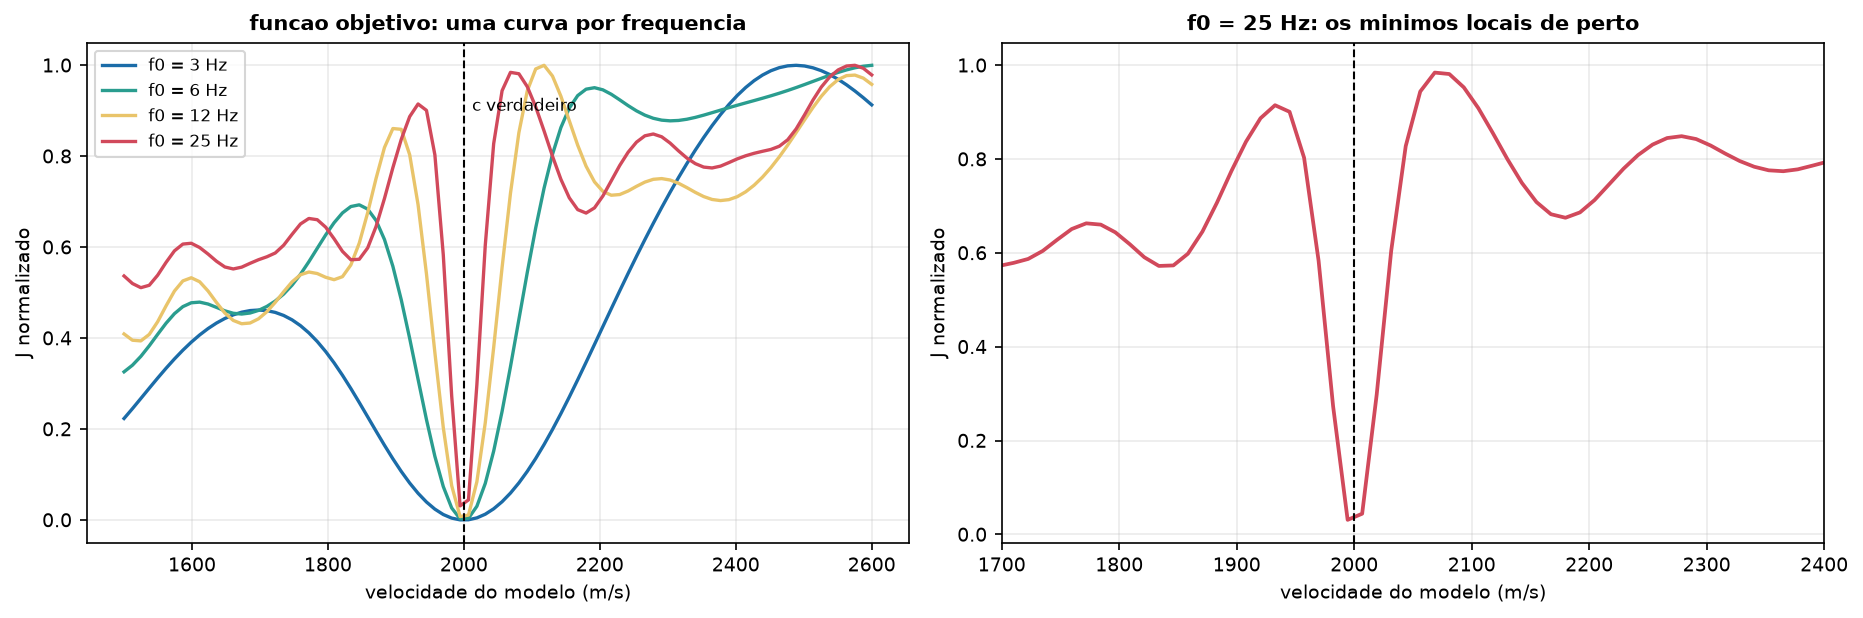
\includegraphics[width=0.96\textwidth]{../saidas/aula07/01_funcao_objetivo.png}
\caption{$J(c)$ varrido para quatro frequ\^encias, meio homog\^eneo,
$c_{\text{verd}} = 2000$\,m/s. A largura do vale central escala com $1/f$,
como prev\^e \eqref{eq:tolerancia3}.}
\end{figure}

Com $\delta t \approx -L\,\delta c/c^{2}$ para um percurso $L$, o crit\'erio
$\abs{\delta t}<T/2$ vira
\begin{equation}
\abs{\delta c} < \frac{c^{2}}{2 f L}.
\label{eq:tolerancia3}
\end{equation}

Valida\c{c}\~ao medida no curso (vale de atra\c{c}\~ao varrido
numericamente):

\begin{center}
\begin{tabular}{@{}rrrr@{}}
\toprule
$f_0$ (Hz) & vale medido (m/s) & semilargura prevista & semilargura medida \\
\midrule
3{,}0  & 1710 a 2489 & 422 & 389 \\
6{,}0  & 1858 a 2192 & 211 & 167 \\
12{,}0 & 1908 a 2118 & 105 & 105 \\
25{,}0 & 1945 a 2069 & 51  & 62 \\
\bottomrule
\end{tabular}
\end{center}

\section{Funcionais alternativos e suas fontes adjuntas}

Trocar o funcional muda \emph{uma \'unica coisa} no c\'odigo: a
\textbf{fonte adjunta} $f_{\text{adj}} = \partial J/\partial d_{\text{cal}}$
injetada nos receptores (Cap.~\ref{cap:adjunto}). Vale, portanto, escrever
cada uma explicitamente.

\subsection*{Envolt\'oria}

Com $\mathcal{H}$ a transformada de Hilbert e
$E = \sqrt{d^{2} + (\mathcal{H}d)^{2}}$ a envolt\'oria,
$J_{\text{env}} = \tfrac12\int (E_{\text{cal}} - E_{\text{obs}})^{2}$.

\begin{derivacao}[A fonte adjunta da envolt\'oria]
De $E^{2} = d^{2}+(\mathcal{H}d)^{2}$ segue
$E\,\delta E = d\,\delta d + (\mathcal{H}d)\,\mathcal{H}(\delta d)$. Com
$\Delta E = E_{\text{cal}}-E_{\text{obs}}$,
\[
\delta J = \int \frac{\Delta E}{E}\Bigl[d\,\delta d
 + (\mathcal{H}d)\,\mathcal{H}(\delta d)\Bigr]\dd t .
\]
Usando que $\mathcal{H}$ \'e \textbf{anti-auto-adjunta}
($\int f\,\mathcal{H}g = -\int \mathcal{H}f\,g$), o segundo termo passa para
$\delta d$ e
\begin{equation}
f_{\text{adj}}^{\text{env}}
 = \frac{\Delta E}{E}\,d
 \;-\; \mathcal{H}\!\left[\frac{\Delta E}{E}\,\mathcal{H}d\right].
\end{equation}
\end{derivacao}

\textbf{Pre\c{c}o.} A envolt\'oria descarta a fase fina, que \'e justamente o
que d\'a resolu\c{c}\~ao. Usa-se nas primeiras bandas e troca-se pelo $L_2$
depois.

\subsection*{Tempo de tr\^ansito por correla\c{c}\~ao cruzada}

Seja $\Delta T$ o atraso que maximiza a correla\c{c}\~ao entre sint\'etico e
observado numa janela, e $J = \tfrac12\sum (\Delta T)^{2}$. A fonte adjunta
(Luo \& Schuster, 1991; Tromp \emph{et al.}, 2005, eqs.~42 e 45) \'e
\begin{equation}
f_{\text{adj}}^{\text{cc}}(t) = -\frac{\Delta T}{N}\,
  \partial_t d_{\text{cal}}(T-t),
\qquad
N = \int_0^T \bigl[\partial_t d_{\text{cal}}(t)\bigr]^{2}\dd t .
\label{eq:adjcc}
\end{equation}

\begin{armadilha}[Duas formas da normaliza\c{c}\~ao, e tr\^es sinais para acertar]
N\~ao \'e raro ver a normaliza\c{c}\~ao escrita como
$N = \int d_{\text{cal}}\,\partial_{tt}d_{\text{cal}}\dd t$. Integrando por
partes, com os termos de fronteira nulos,
\[
\int_0^T d\,\partial_{tt}d \dd t \;=\; -\int_0^T (\partial_t d)^{2}\dd t ,
\]
ou seja: as duas express\~oes s\~ao a mesma coisa \textbf{a menos de um
sinal}. Some a isso a conven\c{c}\~ao adotada para $\Delta T$ (observado menos
sint\'etico, ou o contr\'ario) e o sentido do tempo em que a fonte adjunta \'e
injetada, e h\'a \emph{tr\^es} sinais independentes para acertar.

Use a forma \eqref{eq:adjcc}, em que $N > 0$ por constru\c{c}\~ao, e
\textbf{fixe o sinal com o teste do Cap\'itulo~\ref{cap:verificacao}}, nunca
por inspe\c{c}\~ao. Um sinal trocado aqui produz uma invers\~ao que
\emph{sobe} o funcional com total confian\c{c}a --- e, como o Volume 2
insiste, isso n\~ao se parece com erro.
\end{armadilha}

\textbf{Pre\c{c}o.} Exige \emph{janelamento} --- \'e preciso identificar
\emph{qual} evento se est\'a comparando. Isso reintroduz interpreta\c{c}\~ao
humana, que era justamente o que a FWI prometia eliminar. Em compensa\c{c}\~ao,
$\Phi(\tau) = \tfrac12\tau^{2}$ exatamente: perfeitamente convexa em deslocamento,
dentro da janela.

\subsection*{Invers\~ao adaptativa (AWI)}

Estime o filtro de Wiener $u$ que leva o sint\'etico ao observado,
$u = \argmin_u \norm{u * d_{\text{cal}} - d_{\text{obs}}}^{2}$, e penalize o
\emph{espalhamento} desse filtro:
\begin{equation}
J_{\text{AWI}} = \frac{\norm{T u}^{2}}{\norm{u}^{2}},
\qquad T = \operatorname{diag}(t)
\qquad\text{(Warner \& Guasch, 2016)} .
\end{equation}

A ideia \'e elegante: se o modelo estiver certo, $u$ \'e uma delta em
$t=0$ e $J = 0$; se estiver errado, $u$ concentra-se em $t = \tau \ne 0$ e $J$
cresce como $\tau^{2}$ --- \textbf{sem precisar janelar}, porque o filtro
encontra o atraso sozinho. O denominador torna $J$ invariante a escala.

\textbf{Pre\c{c}o.} Um problema de m\'inimos quadrados adicional por
tra\c{c}o, e um par\^ametro de regulariza\c{c}\~ao na estimativa de $u$.

\subsection*{Transporte \'otimo}

\begin{teoria}[Por que o transporte \'otimo \'e o candidato natural, e por que
\'e dif\'icil]
Para duas densidades de probabilidade $\mu,\nu$ em $\Real$, a dist\^ancia de
Wasserstein quadr\'atica \'e
\[
W_2^{2}(\mu,\nu) = \inf_{\pi}\int \abs{x-y}^{2}\dd\pi(x,y),
\]
com $\pi$ percorrendo os acoplamentos de $\mu$ e $\nu$. Em 1D ela tem forma
fechada via fun\c{c}\~oes de distribui\c{c}\~ao acumuladas.

\textbf{A propriedade decisiva:} para uma transla\c{c}\~ao pura,
$W_2(\mu, \mu(\cdot-\tau)) = \abs{\tau}$, logo $W_2^{2} = \tau^{2}$ ---
\textbf{exatamente convexa em deslocamento}, para qualquer $\tau$, sem janela
e sem limite de meio ciclo. \'E o comportamento que se queria desde o
in\'icio deste cap\'itulo.

\textbf{O obst\'aculo:} $W_2$ \'e definida para medidas \textbf{positivas} e
de \textbf{massa igual}. Um tra\c{c}o s\'ismico oscila em torno de zero e
n\~ao \'e nenhuma das duas coisas. Os contornos usados na literatura --- cada
um com o seu custo --- s\~ao: separar as partes positiva e negativa;
transformar por $d\mapsto d^{2}$, $d \mapsto e^{\beta d}$ ou $d\mapsto d + c$;
ou aplicar OT no \emph{gr\'afico} do
tra\c{c}o (\emph{graph-space OT}), que preserva a propriedade ao custo de um
problema de atribui\c{c}\~ao por tra\c{c}o.

Para uma transla\c{c}\~ao \emph{pura} numa janela longa, uma
transforma\c{c}\~ao ponto a ponto $g$ com $g(0)=0$ (como $d^{2}$) comuta com a
transla\c{c}\~ao e preserva $W_2^{2} = \tau^{2}$. O custo aparece fora desse
caso ideal: $d^{2}$ descarta a polaridade; $e^{\beta d}$ e $d+c$ criam um fundo
constante que n\~ao se translada numa janela finita e achata o funcional; e
nenhuma transforma\c{c}\~ao ponto a ponto \'e neutra para varia\c{c}\~oes de
amplitude.

\textbf{A leitura honesta:} o transporte \'otimo resolve o problema de
deslocamento de forma limpa \emph{no caso idealizado}, e a dificuldade toda
migra para a transforma\c{c}\~ao que torna o dado admiss\'ivel. Nenhuma dessas
transforma\c{c}\~oes \'e neutra.
\end{teoria}

\section{Dom\'inio estendido: mudar o espa\c{c}o em vez do funcional}
\label{sec:wri}

\begin{teoria}[WRI: relaxar a EDP]
Todos os funcionais acima permanecem na forma \emph{reduzida}: a EDP \'e
satisfeita exatamente, e a n\~ao convexidade fica em $J$. A alternativa
estrutural \'e relaxar essa restri\c{c}\~ao:
\begin{equation}
\min_{m,u}\
 \tfrac12\norm{Ru - d_{\text{obs}}}^{2}
 + \tfrac{\mu}{2}\norm{\mathcal{A}(m)u - f}^{2} .
\label{eq:wri}
\end{equation}

Para $m$ fixo, \eqref{eq:wri} \'e \textbf{quadr\'atica} em $u$: resolve-se em
um passo (um problema de m\'inimos quadrados aumentado). Para $u$ fixo, o
res\'iduo da EDP \'e \textbf{linear} em $m$ (lembre que a equa\c{c}\~ao \'e
linear em $m=1/c^{2}$), de modo que a atualiza\c{c}\~ao de $m$ tamb\'em \'e um
problema linear.

O ganho: o campo $u$ n\~ao \'e mais obrigado a ser uma solu\c{c}\~ao
f\'isica do modelo atual. Ele pode \emph{j\'a} ajustar o dado, e o res\'iduo da
EDP passa a indicar onde o modelo precisa mudar --- um caminho que contorna o
$\abs{\delta t}>T/2$ em vez de enfrent\'a-lo.

O pre\c{c}o, e ele \'e s\'erio: armazenar e resolver para $u$ em todo o
dom\'inio e todo o tempo, para cada tiro. Em 3D isso \'e proibitivo com a
tecnologia atual, e \'e por isso que WRI \'e, hoje, sobretudo um resultado 2D.
E $\mu$ \'e mais um par\^ametro livre, cuja trajet\'oria de continua\c{c}\~ao
($\mu$ crescendo at\'e recuperar a forma reduzida) precisa ser projetada.
\end{teoria}

\begin{pratica}[Ordem de prioridade, que n\~ao muda com o n\'ivel de
sofistica\c{c}\~ao]
1.~Baixe a frequ\^encia inicial. \quad 2.~Melhore o modelo inicial. \quad
3.~\emph{S\'o ent\~ao} troque o funcional ou estenda o dom\'inio.

Cada item desta lista introduz mais par\^ametros livres que o anterior, e
portanto mais maneiras de produzir um resultado que parece bom e n\~ao \'e.
\end{pratica}

\begin{resumo}
\begin{itemize}[leftmargin=*, itemsep=1pt]
\item $\Phi(\tau) = \norm{d}^{2} - R_{dd}(\tau)$: a n\~ao convexidade \emph{\'e}
a autocorrela\c{c}\~ao do dado. Para uma Ricker, divisa em $0{,}43\,T$ e
m\'inimo local em $0{,}91\,T$.
\item Cada funcional alternativo se reduz a uma fonte adjunta diferente ---
deduzida aqui para envolt\'oria e correla\c{c}\~ao cruzada.
\item $W_2^{2}$ \'e exatamente convexa em transla\c{c}\~ao, mas exige
positividade: a dificuldade migra para a transforma\c{c}\~ao do dado.
\item WRI muda o \emph{espa\c{c}o} em vez do funcional; custo de mem\'oria
proibitivo em 3D.
\end{itemize}
\end{resumo}

% =====================================================================
\chapter{Estado adjunto, Born e n\'ucleos de sensibilidade}
\label{cap:adjunto}

\begin{ideia}
Tr\^es objetos que a literatura trata como assuntos separados --- o m\'etodo
do estado adjunto, a aproxima\c{c}\~ao de Born e a migra\c{c}\~ao reversa no
tempo --- s\~ao a \emph{mesma} coisa vista de tr\^es \^angulos:
respectivamente, o algoritmo que aplica $F'^{*}$, a f\'ormula expl\'icita de
$F'$, e a interpreta\c{c}\~ao de $F'^{*}r$ como imagem. Este cap\'itulo
estabelece a equival\^encia.
\end{ideia}

\begin{matematica}[distribui\c{c}\~oes, fun\c{c}\~ao de Green e a s\'erie de Born]
\textbf{Distribui\c{c}\~oes.} $\delta(\mathbf{x}-\mathbf{x}_0)$ n\~ao \'e uma
fun\c{c}\~ao: \'e o funcional linear $\varphi \mapsto \varphi(\mathbf{x}_0)$. A
utilidade aqui \'e dupla: representa fontes e receptores pontuais, e permite
escrever ``avaliar no receptor'' como uma integral --- o que torna leg\'itimo
derivar sob o sinal de integral na dedu\c{c}\~ao seguinte.

\textbf{Fun\c{c}\~ao de Green.} Para o operador de onda
$\mathcal{A}(m) = m\,\partial_{tt} - \nabla^{2}$, a fun\c{c}\~ao de Green
$G(\mathbf{x},t;\mathbf{x}',t')$ resolve
\[
\mathcal{A}(m)\,G = \delta(\mathbf{x}-\mathbf{x}')\,\delta(t-t'),
\]
com condi\c{c}\~oes iniciais nulas. Ela \'e o \emph{n\'ucleo} do operador
inverso: $u = \mathcal{A}^{-1}f$ escreve-se
$u(\mathbf{x},t) = \int G * f$.

Duas propriedades s\~ao usadas adiante. \textbf{Reciprocidade}:
$G(\mathbf{x},t;\mathbf{x}',t') = G(\mathbf{x}',t;\mathbf{x},t')$ --- trocar
fonte e receptor n\~ao muda nada, e \'e por isso que retropropagar a partir dos
receptores faz sentido f\'isico. \textbf{Causalidade}: $G = 0$ para $t<t'$, o
que faz a integral temporal ter limites finitos.

\textbf{S\'erie de Born.} Escreva $m = m_0 + \delta m$. Como
$\mathcal{A}(m) = \mathcal{A}(m_0) + \delta m\,\partial_{tt}$, a identidade
$\mathcal{A}(m)u = f$ com $u = u_0 + \delta u$ d\'a exatamente
\[
\mathcal{A}(m_0)\,\delta u = -\,\delta m\;\partial_{tt} u
 = -\,\delta m\;\partial_{tt} u_0
   \;-\;\delta m\;\partial_{tt}\delta u .
\]
Iterando, obt\'em-se a s\'erie de Neumann (s\'erie de Born):
o primeiro termo \'e espalhamento simples, o segundo \'e espalhamento duplo, e
assim por diante. \textbf{Truncar no primeiro termo \'e a aproxima\c{c}\~ao de
Born}, e \'e \emph{exatamente} a lineariza\c{c}\~ao $F'(m_0)\delta m$ ---
n\~ao uma aproxima\c{c}\~ao adicional.

A s\'erie converge quando o espalhamento \'e fraco. Em FWI ela n\~ao converge
para contrastes fortes --- e \'e por isso que a FWI \emph{n\~ao} \'e uma
migra\c{c}\~ao de m\'inimos quadrados: ela reintroduz, a cada itera\c{c}\~ao,
os termos de ordem superior, resolvendo de novo a EDP completa.
\end{matematica}

\section{O operador de Born, explicitamente}

No dom\'inio da frequ\^encia, com $\mathcal{A}_\omega(m) = -\omega^{2}m -
\nabla^{2}$, perturbar $m \to m+\delta m$ d\'a
$\mathcal{A}_\omega\,\delta\hat u = \omega^{2}\,\delta m\,\hat u_0$, e
portanto
\begin{equation}
\boxed{\;
\bigl[F'(m)\,\delta m\bigr](\mathbf{x}_r,\omega)
 = \omega^{2}\!\int_{\Omega} G(\mathbf{x}_r,\mathbf{x};\omega)\;
   \delta m(\mathbf{x})\;\hat u_0(\mathbf{x},\omega)\dd\mathbf{x} \;}
\label{eq:born}
\end{equation}

Esta \'e a \textbf{integral de espalhamento}. Lida como algoritmo: para cada
ponto $\mathbf{x}$, tome o campo incidente $\hat u_0$ ali, multiplique pela
perturba\c{c}\~ao, e propague at\'e o receptor com $G$.

\begin{teoria}[As duas maneiras de calcular o gradiente, e por que uma \'e
usada]
De \eqref{eq:born}, o adjunto sai por inspe\c{c}\~ao, usando reciprocidade:
\begin{equation}
\bigl[F'^{*}r\bigr](\mathbf{x})
 = \operatorname{Re}\int\!\dd\omega\;\omega^{2}\,
   \overline{\hat u_0(\mathbf{x},\omega)}
   \sum_r \overline{G(\mathbf{x},\mathbf{x}_r;\omega)}\;\hat r(\mathbf{x}_r,\omega).
\label{eq:adj_freq}
\end{equation}

Duas implementa\c{c}\~oes s\~ao poss\'iveis, e a escolha \'e de custo e de
armazenamento:

\textbf{(i) Integral de espalhamento.} Calcule e armazene
$G(\mathbf{x},\mathbf{x}_r)$ para \emph{cada} receptor --- $n_r$
modelagens, feitas \emph{uma vez} e reaproveitadas por todos os tiros e todas
as itera\c{c}\~oes (por reciprocidade) --- e some. Pre\c{c}o: guardar $n_r$
campos de Green em todo o dom\'inio.

\textbf{(ii) Estado adjunto.} Reconhe\c{c}a que
$\sum_r \overline{G(\mathbf{x},\mathbf{x}_r)}\hat r(\mathbf{x}_r)$ \'e
\emph{a solu\c{c}\~ao de uma \'unica equa\c{c}\~ao de onda} com todos os
res\'iduos como fontes simult\^aneas. Custo: \textbf{1} modelagem adjunta por
tiro, a cada itera\c{c}\~ao, sem armazenamento extra.

Por itera\c{c}\~ao, portanto, (ii) custa $n_s$ propaga\c{c}\~oes adjuntas e
(i) nenhuma, depois de pagar $n_r$ de uma vez. Com muito mais fontes que
receptores e disco barato --- sismologia regional --- a integral de
espalhamento sai mais econ\^omica (Chen, Jordan \& Zhao, 2007); em
explora\c{c}\~ao, com milhares de receptores por tiro, o estado adjunto vence
com folga. \textbf{O
m\'etodo do estado adjunto n\~ao \'e uma aproxima\c{c}\~ao da integral de
espalhamento: \'e a mesma quantidade, avaliada por uma associa\c{c}\~ao mais
econ\^omica dos fatores.} A distin\c{c}\~ao \'e a mesma entre
$(\mathbf{a}^{T}B)\mathbf{c}$ e $\mathbf{a}^{T}(B\mathbf{c})$.
\end{teoria}

\section{A dedu\c{c}\~ao pelo Lagrangiano, com os termos de fronteira}

\begin{derivacao}[Dedu\c{c}\~ao completa]
Com a restri\c{c}\~ao $\mathcal{F}(p,m) = m\,\partial_{tt}p - \nabla^{2}p - s
= 0$ e condi\c{c}\~oes iniciais nulas,
\[
\mathcal{L} = J(p) + \int_{\Omega}\!\!\int_{0}^{T}
\lambda\,\bigl[m\,\partial_{tt}p - \nabla^{2}p - s\bigr]\dd t\dd\mathbf{x}.
\]

\textbf{Varia\c{c}\~ao em $p$.} Com
$J = \tfrac12\int\!\!\int\sum_r\delta(\mathbf{x}-\mathbf{x}_r)(p-d_{\text{obs}})^{2}$,
\[
\delta\mathcal{L}
 = \int\!\!\int\Bigl[\underbrace{\sum_r\delta(\mathbf{x}-\mathbf{x}_r)\,r}_{\text{de }J}
 + m\,\partial_{tt}\lambda - \nabla^{2}\lambda\Bigr]\delta p
 \;+\; \mathcal{B}_t \;+\; \mathcal{B}_x ,
\]
onde, ap\'os integrar por partes duas vezes em $t$ e aplicar a segunda
identidade de Green em $\mathbf{x}$,
\[
\mathcal{B}_t = \int_\Omega \Bigl[\lambda\,m\,\partial_t\delta p
 - m\,\partial_t\lambda\,\delta p\Bigr]_{t=0}^{t=T}\dd\mathbf{x},
\qquad
\mathcal{B}_x = -\int_0^T\!\!\oint_{\partial\Omega}
 \bigl(\lambda\,\partial_n\delta p - \delta p\,\partial_n\lambda\bigr)\dd S\dd t .
\]

\textbf{$\mathcal{B}_t$.} Em $t=0$ ele se anula porque as condi\c{c}\~oes
iniciais s\~ao fixas: $\delta p = \partial_t\delta p = 0$. Em $t=T$,
$\delta p$ e $\partial_t\delta p$ s\~ao \emph{livres}, logo a \'unica maneira
de anular \'e impor
\[
\lambda(\cdot,T) = \partial_t\lambda(\cdot,T) = 0 .
\]
\textbf{\'E da\'i que v\^em as condi\c{c}\~oes finais} --- n\~ao de
conven\c{c}\~ao.

\textbf{$\mathcal{B}_x$.} Anula-se se $\lambda$ satisfizer, em
$\partial\Omega$, a condi\c{c}\~ao \textbf{adjunta} \`a do problema direto.
Dirichlet homog\^enea ($p=0$) e Neumann homog\^enea s\~ao auto-adjuntas; uma
camada absorvente n\~ao \'e (Cap.~\ref{cap:bordas}).

\textbf{Equa\c{c}\~ao adjunta.} Anulando o colchete:
\begin{equation}
m\,\partial_{tt}\lambda - \nabla^{2}\lambda
 = -\sum_r r(t)\,\delta(\mathbf{x}-\mathbf{x}_r),
\qquad
\lambda(\cdot,T) = \partial_t\lambda(\cdot,T) = 0 .
\label{eq:adjunta3}
\end{equation}

\textbf{Gradiente.} Sobra o termo expl\'icito em $m$:
\begin{equation}
\frac{\partial J}{\partial m}(\mathbf{x})
 = \int_{0}^{T}\lambda(\mathbf{x},t)\,\partial_{tt}p(\mathbf{x},t)\dd t ,
\label{eq:grad3}
\end{equation}
somado sobre tiros, e com pesos de quadratura $\Delta h^{d}\Delta t$ na forma
discreta.
\end{derivacao}

\begin{teoria}[Por que o operador de onda ac\'ustico \'e auto-adjunto]
Compare \eqref{eq:adjunta3} com o problema direto: \emph{mesma} equa\c{c}\~ao.
A raz\~ao \'e estrutural: $\partial_{tt}^{*} = \partial_{tt}$ (duas
integra\c{c}\~oes por partes, dois sinais que se cancelam) e
$(\nabla^{2})^{*} = \nabla^{2}$ com contorno homog\^eneo. Derivadas de ordem
\emph{par}, com coeficientes em forma divergente --- como $m(\mathbf{x})\,
\partial_{tt}$ e $\nabla\!\cdot\!(\rho^{-1}\nabla)$ --- d\~ao operador
auto-adjunto. (A forma importa: $a(x)\,\partial_{xx}$ \emph{n\~ao} \'e, porque o
seu adjunto \'e $\partial_{xx}(a\,\cdot)$.)

Basta uma derivada \emph{\'impar} para quebrar: $\partial_t^{*} =
-\partial_t$. \'E o caso do termo dissipativo viscoac\'ustico
(Cap.~\ref{cap:limites}), do sistema de primeira ordem velocidade--tens\~ao (em
que o adjunto troca o sinal do acoplamento), e da CPML.
\end{teoria}

\section{N\'ucleos de sensibilidade}

Substituindo em \eqref{eq:grad3} as representa\c{c}\~oes por fun\c{c}\~ao de
Green de $p$ e de $\lambda$, o gradiente escreve-se como uma soma, sobre pares
fonte--receptor e frequ\^encias, de \textbf{n\'ucleos de sensibilidade}
\begin{equation}
K^{sr}(\mathbf{x},\omega) \;=\; \operatorname{Re}\Bigl[\,\omega^{2}\,
 \overline{\hat w(\omega)}\;
 \overline{G(\mathbf{x},\mathbf{x}_s;\omega)}\;
 \overline{G(\mathbf{x},\mathbf{x}_r;\omega)}\;
 \hat r(\mathbf{x}_r,\omega)\Bigr],
\label{eq:kernel}
\end{equation}
com $\hat w$ a ondaleta e $\hat r$ o res\'iduo naquele receptor.

Escrevendo $G \sim A\,e^{-\mathrm{i}\omega T}$ (um atraso $T$, na
conven\c{c}\~ao de Fourier do volume), o produto dos dois conjugados carrega a
fase $+\omega[T_s(\mathbf{x}) + T_r(\mathbf{x})]$, e um evento do res\'iduo no
instante $t$ carrega $-\omega t$. A fase total de \eqref{eq:kernel} \'e
portanto $-\omega\,[\,t - T_s(\mathbf{x}) - T_r(\mathbf{x})\,]$ --- e \'e a sua
estacionariedade que seleciona a geometria.

\begin{teoria}[A geometria que a fase estacion\'aria imp\~oe]
Quando a fase de \eqref{eq:kernel} varia r\'apido com $\omega$, a integral
sobre a banda cancela. Sobram os pontos em que ela \'e \emph{estacion\'aria},
isto \'e $t \approx T_s(\mathbf{x}) + T_r(\mathbf{x})$ para os tempos $t$ em
que o res\'iduo tem energia. Duas geometrias saem disso:

\textbf{Is\'ocronas (ondas espalhadas/refletidas).} O lugar
$T_s(\mathbf{x}) + T_r(\mathbf{x}) = t_{\text{obs}}$ \'e, em meio homog\^eneo,
uma \textbf{elipse} com focos na fonte e no receptor. \'E o arco que aparece
nas figuras de gradiente.

\textbf{Banana (ondas transmitidas).} Para uma chegada direta, a regi\~ao de
fase estacion\'aria \'e um tubo em torno do raio geom\'etrico, com largura
$\sim\sqrt{\lambda L}$ --- a \textbf{zona de Fresnel}.

\textbf{O ``buraco'' no meio da banana.} Para um desajuste de tempo de
tr\^ansito puro (correla\c{c}\~ao cruzada), a sensibilidade \emph{anula-se
sobre o pr\'oprio raio} e \'e m\'axima num anel ao redor --- o n\'ucleo
\emph{banana-doughnut} (Marquering \emph{et al.}, 1999; Tromp \emph{et al.},
2005). N\~ao \'e curiosidade: contradiz frontalmente a
intui\c{c}\~ao da teoria de raios, segundo a qual a sensibilidade estaria
concentrada no raio. A resolu\c{c}\~ao finita da FWI \'e consequ\^encia
direta desta estrutura --- a onda \'e sens\'ivel a um \emph{volume}.
\end{teoria}

\begin{figure}[htbp]
\centering
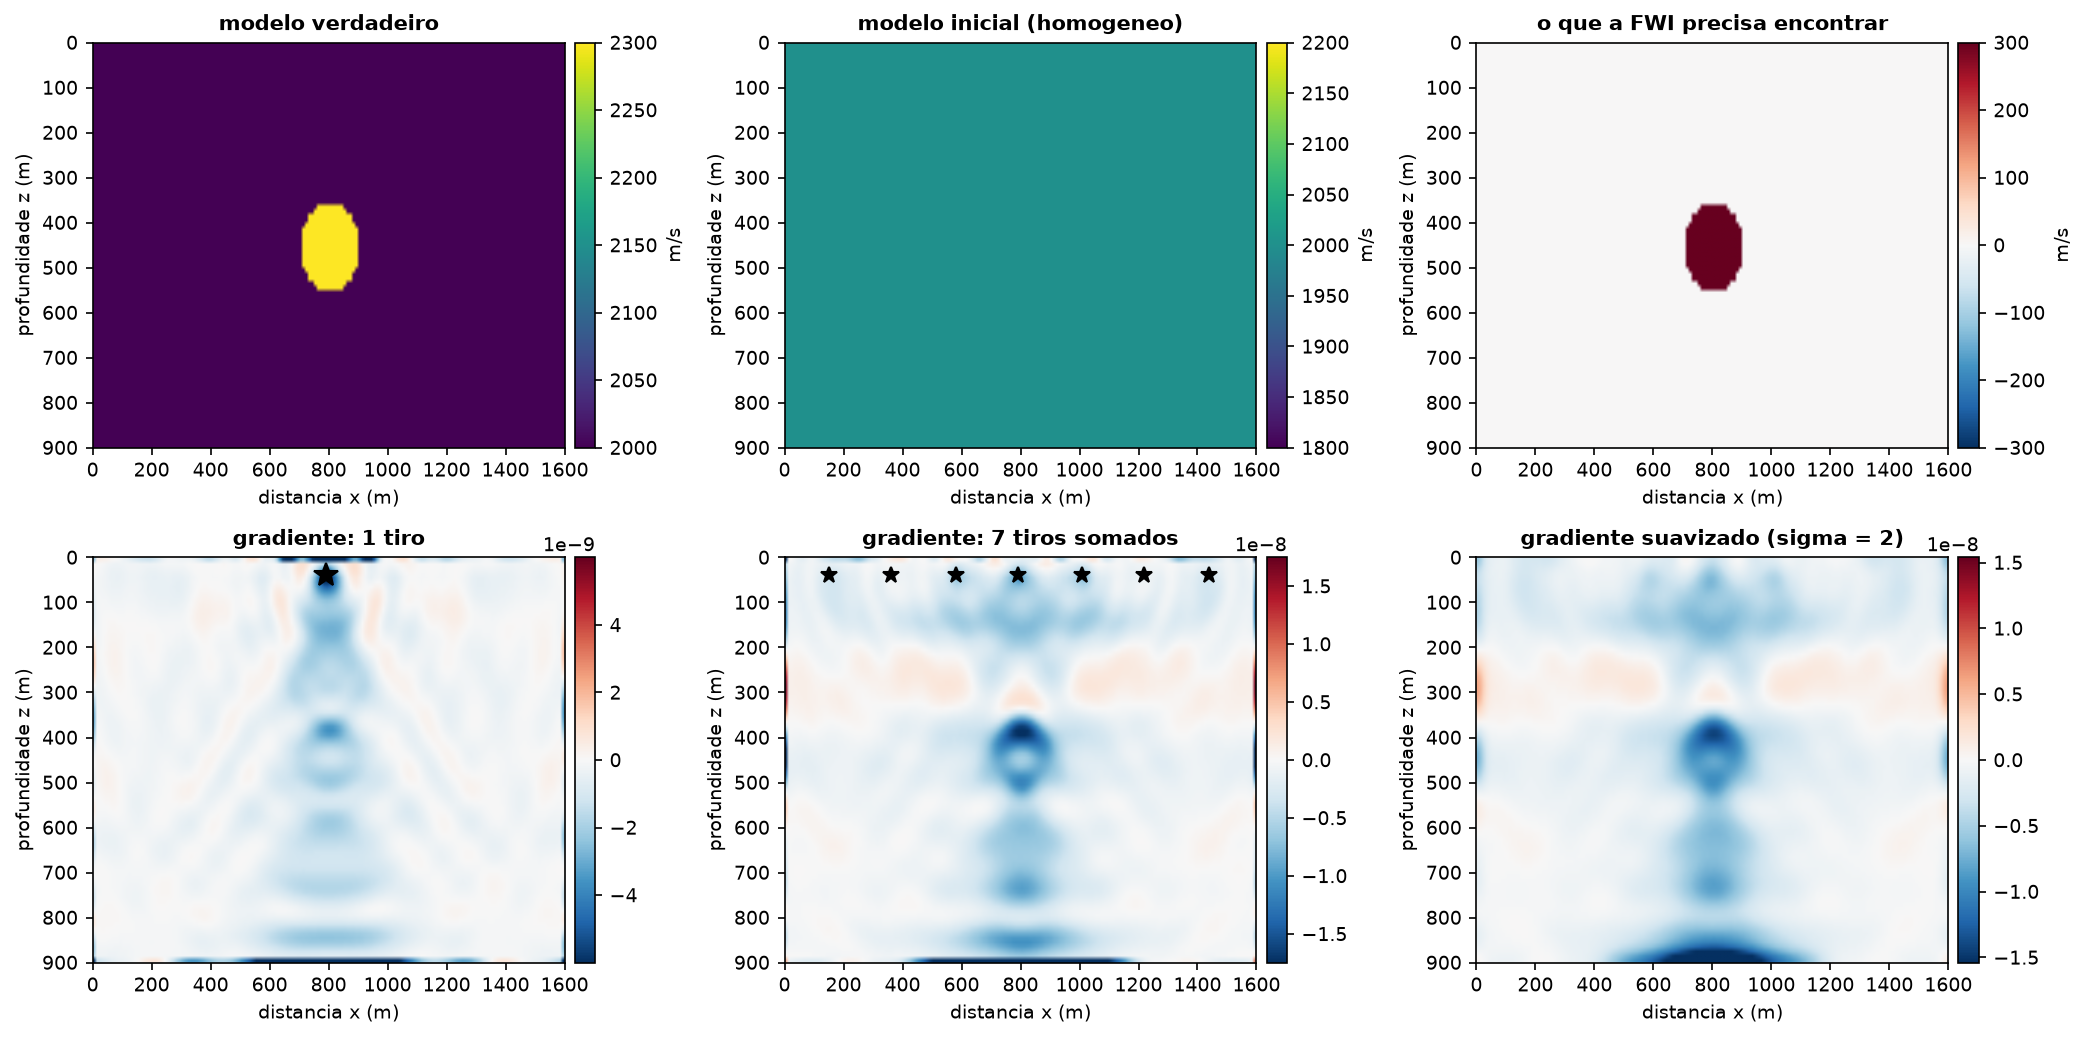
\includegraphics[width=0.96\textwidth]{../saidas/aula08/01_gradiente_adjunto.png}
\caption{Gradiente adjunto calculado pelo c\'odigo do curso: um tiro
(esquerda), sete tiros somados (centro), suavizado (direita). Os arcos s\~ao
as is\'ocronas previstas pela an\'alise de fase estacion\'aria; a soma sobre
tiros \'e o que colapsa a ambiguidade.}
\end{figure}

\section{Decomposi\c{c}\~ao do gradiente: tomogr\'afico e de migra\c{c}\~ao}
\label{sec:rwi}

\begin{teoria}[Duas contribui\c{c}\~oes com n\'umeros de onda opostos]
A correla\c{c}\~ao \eqref{eq:grad3} soma contribui\c{c}\~oes de \emph{todos} os
pontos onde os dois campos coincidem. Elas se separam naturalmente em duas
fam\'ilias, com propriedades opostas:

\textbf{(a) Contribui\c{c}\~ao de migra\c{c}\~ao} (ou ``de reflex\~ao''). O
campo direto \emph{descendo} encontra o campo adjunto \emph{subindo}, num
ponto de refletor. O \^angulo de espalhamento \'e pr\'oximo de $\pi$, e por
\eqref{eq:km} o n\'umero de onda impresso \'e \textbf{alto}: o gradiente
desenha a \emph{interface}. \'E, literalmente, a condi\c{c}\~ao de imagem da
RTM.

\textbf{(b) Contribui\c{c}\~ao tomogr\'afica.} Os dois campos viajam
aproximadamente na \emph{mesma} dire\c{c}\~ao ao longo do trajeto que liga
fonte e receptor --- \^angulo de espalhamento pr\'oximo de zero, n\'umero de
onda \textbf{baixo}. O gradiente atualiza o \emph{fundo} de velocidade, ao
longo dos ``arcos de banana''.

Em um \'unico gradiente as duas est\~ao \textbf{superpostas}, e t\^em
amplitudes muito diferentes: a de migra\c{c}\~ao domina, porque as
reflex\~oes s\~ao eventos bem localizados e de alta frequ\^encia.
\end{teoria}

\begin{armadilha}[Por que isso \'e um problema pr\'atico, e n\~ao apenas
uma taxonomia]
O que a FWI mais precisa construir --- e n\~ao consegue --- \'e o
\emph{fundo} de velocidade, a parte de baixo n\'umero de onda que preenche a
lacuna espectral da §\ref{sec:cobertura}. Essa informa\c{c}\~ao est\'a na
contribui\c{c}\~ao tomogr\'afica (b), que \'e a mais fraca das duas.

Resultado: com dado dominado por reflex\~oes (aquisi\c{c}\~ao de afastamento
curto), o gradiente \'e essencialmente uma imagem de migra\c{c}\~ao. A
invers\~ao acrescenta detalhe de alta frequ\^encia sobre um fundo
\textbf{errado}, e o detalhe fica no lugar errado --- com $J$ caindo o tempo
todo.

\textbf{Sintoma reconhec\'ivel:} o modelo final parece uma migra\c{c}\~ao
sobreposta ao modelo inicial, com os refletores n\'itidos e a tend\^encia de
velocidade praticamente intocada.
\end{armadilha}

\begin{pratica}[RWI: separar as duas em vez de somar]
A \textbf{invers\~ao de forma de onda por reflex\~ao} (RWI, e a fam\'ilia de
m\'etodos de an\'alise de velocidade por equa\c{c}\~ao de onda) explora a
separa\c{c}\~ao explicitamente. O esquema comum:
\begin{enumerate}[leftmargin=*, itemsep=1pt]
\item construa uma \emph{refletividade} a partir do modelo atual (uma
migra\c{c}\~ao);
\item gere o campo refletido com essa refletividade, tratando-a como fonte
secund\'aria;
\item correlacione o campo \emph{refletido} com o adjunto --- o que isola a
contribui\c{c}\~ao (b), tomogr\'afica, porque ambos percorrem o mesmo trajeto
descendente;
\item atualize apenas o fundo de velocidade com esse gradiente, mantendo a
refletividade fixa; alterne.
\end{enumerate}

O ganho \'e claro: constr\'oi-se o baixo n\'umero de onda a partir de
\emph{reflex\~oes}, sem depender de ondas mergulhantes --- isto \'e, sem
depender de afastamento longo.

O pre\c{c}o tamb\'em: a separa\c{c}\~ao entre ``fundo'' e ``refletividade'' \'e
uma escolha do usu\'ario (tipicamente um corte de n\'umero de onda), e o
resultado depende dela. \'E mais um par\^ametro que precisa ser declarado.
\end{pratica}

\section{Gradiente multipar\^ametro}

Para um vetor de par\^ametros $\mathbf{p} = (p_1,\dots,p_K)$, o mesmo
Lagrangiano d\'a \emph{um} campo adjunto e $K$ gradientes,
\begin{equation}
\frac{\partial J}{\partial p_k}(\mathbf{x})
 = \int_0^T \lambda\,
   \frac{\partial \mathcal{A}}{\partial p_k}\,p \dd t ,
\end{equation}
isto \'e: o custo \textbf{n\~ao} cresce com o n\'umero de par\^ametros --- s\'o
a correla\c{c}\~ao final \'e refeita com um operador diferente.

\begin{armadilha}[Onde a regra da cadeia costuma ser esquecida]
Se o c\'odigo inverte em $\mathbf{q} = \Phi(\mathbf{p})$ mas propaga em
$\mathbf{p}$, o gradiente correto \'e $\Phi'^{T}\mathbf{g}_{\mathbf{p}}$ ---
com a \textbf{jacobiana completa}, n\~ao termo a termo. Exemplo concreto: num
solver el\'astico parametrizado por $(v_p,v_s,\rho)$, a densidade entra em
$\lambda$, em $\mu$ \emph{e} no termo de in\'ercia, de modo que
$\partial J/\partial\rho$ tem tr\^es contribui\c{c}\~oes. Manter apenas uma
produz um gradiente est\'avel e errado --- a assinatura t\'ipica de raz\~ao
constante $\ne 1$ no teste do Cap\'itulo~\ref{cap:verificacao}.

Um caso instrutivo: em alguns c\'odigos el\'asticos, o gradiente de $v_s$ sai
identicamente nulo quando $v_s = 0$ no modelo. Isso \emph{n\~ao} \'e
propriedade do adjunto: \'e a regra da cadeia, porque
$\partial\mu/\partial v_s = 2\rho v_s$ se anula. A distin\c{c}\~ao importa,
porque sugere o conserto certo (reparametrizar) em vez do errado (procurar
\emph{bug} no adjunto).
\end{armadilha}

\section{Adjunto do programa e \emph{checkpointing}}

O gradiente \eqref{eq:grad3} exige $p$ e $\lambda$ no mesmo instante, com
sentidos de tempo opostos.

\begin{teoria}[\emph{Revolve}: o \'otimo \'e conhecido]
Com $n$ passos de tempo e mem\'oria para $c$ estados, o algoritmo
\emph{revolve} (Griewank \& Walther) atinge o \'otimo te\'orico do compromisso
mem\'oria$\times$recomputa\c{c}\~ao: com $c$ pontos de controle e $r$ sweeps
extras de recomputa\c{c}\~ao, ele cobre
\[
n = \binom{c+r}{c}
\]
passos. A leitura pr\'atica: como o binomial cresce muito r\'apido, um
n\'umero \emph{logar\'itmico} de pontos de controle basta para um fator de
recomputa\c{c}\~ao pequeno --- t\'ipicamente 2 a 3 modelagens extras.

\textbf{Consequ\^encia em 3D.} Um modelo $500\times500\times300$ com
$n_t = 5000$ exigiria $\sim 1{,}5$\,TB por tiro para guardar tudo. Com
\emph{revolve} e algumas dezenas de pontos de controle, cai para dezenas de
GB ao custo de $\sim 2\times$ em computa\c{c}\~ao. \'E por isso que todo
c\'odigo de FWI 3D usa \emph{checkpointing}.

\textbf{E a alternativa que n\~ao serve sempre.} Reconstruir o campo direto
propagando-o ao contr\'ario a partir do estado final custa mem\'oria
$\mathcal{O}(\text{contorno})$ e \'e exata \emph{se} o operador for
revers\'ivel no tempo. Em meio dissipativo \textbf{n\~ao \'e}: reverter a
dissipa\c{c}\~ao \'e amplificar, e o erro de arredondamento cresce
exponencialmente. Ver §\ref{sec:adjunto-visco3}.
\end{teoria}

\begin{resumo}
\begin{itemize}[leftmargin=*, itemsep=1pt]
\item Born \'e $F'$ exatamente (truncar a s\'erie de Neumann no 1\textsuperscript{o}
termo); estado adjunto \'e $F'^{*}$ avaliado com associa\c{c}\~ao econ\^omica;
RTM \'e $F'^{*}r$ interpretado como imagem.
\item As condi\c{c}\~oes finais do adjunto saem do termo de fronteira em
$t=T$, e as condi\c{c}\~oes de contorno adjuntas do termo em $\partial\Omega$.
\item Fase estacion\'aria d\'a as is\'ocronas (reflex\~ao), a banana
(transmiss\~ao) e o buraco central no n\'ucleo de tempo de tr\^ansito.
\item Multipar\^ametro custa o mesmo em propaga\c{c}\~ao; o que muda \'e a
regra da cadeia --- e \'e onde os erros acontecem.
\end{itemize}
\end{resumo}

\begin{exercicio}[Problemas]
\begin{enumerate}[leftmargin=*, itemsep=2pt]
\item Deduza \eqref{eq:born} partindo de $\mathcal{A}_\omega(m)\hat u = \hat s$
e mantendo apenas o primeiro termo da s\'erie de Neumann. Onde exatamente
entra a hip\'otese de espalhamento fraco?
\item Verifique, a partir de \eqref{eq:born}, que $F'^{*}$ dado por
\eqref{eq:adj_freq} satisfaz $\inner{F'\delta m}{r} = \inner{\delta m}{F'^{*}r}$.
Qual propriedade de $G$ \'e usada?
\item Mostre que, para o operador $m\partial_{tt}-\nabla^{2}$ com
condi\c{c}\~oes homog\^eneas, o adjunto \'e ele mesmo. Repita para
$m\partial_{tt} + b\,\partial_t - \nabla^{2}$ e identifique o que muda.
\item Um c\'odigo el\'astico parametrizado em $(v_p,v_s,\rho)$ devolve
$\partial J/\partial v_s \equiv 0$ num modelo com $v_s = 0$. Isso \'e
\emph{bug}? Justifique com a regra da cadeia e proponha a reparametriza\c{c}\~ao
que evita o problema.
\end{enumerate}
\textbf{Respostas.} (1) O termo descartado \'e
$-\delta m\,\partial_{tt}\delta u$, de segunda ordem em $\delta m$: a
hip\'otese \'e que a onda espalhada seja pequena diante da incidente ao longo
de \emph{todo} o percurso --- o que falha em contrastes fortes, e n\~ao apenas
em contrastes locais. (2) Reciprocidade,
$G(\mathbf{x}_r,\mathbf{x}) = G(\mathbf{x},\mathbf{x}_r)$; sem ela, o adjunto
exigiria uma fun\c{c}\~ao de Green distinta e a retropropaga\c{c}\~ao a partir
dos receptores n\~ao seria leg\'itima. (3) $\partial_{tt}^{*}=\partial_{tt}$ e
$(\nabla^{2})^{*}=\nabla^{2}$; com o termo $b\,\partial_t$, como
$\partial_t^{*}=-\partial_t$, o adjunto \'e $m\partial_{tt}-b\partial_t-\nabla^{2}$
--- que, na vari\'avel revertida $\tau = T-t$, volta a ser dissipativo.
(4) N\~ao \'e \emph{bug}: $\partial\mu/\partial v_s = 2\rho v_s$ anula-se em
$v_s=0$, de modo que o zero vem da regra da cadeia, n\~ao do adjunto.
Parametrizar em $\mu$ (ou em $I_s = \rho v_s$) mant\'em sensibilidade n\~ao
nula.
\end{exercicio}

% =====================================================================
\chapter{Verifica\c{c}\~ao}
\label{cap:verificacao}

\begin{ideia}
H\'a dois testes independentes, e eles verificam coisas diferentes: o teste do
produto escalar verifica que o \emph{adjunto} est\'a correto; o teste de
Taylor verifica que a \emph{lineariza\c{c}\~ao} est\'a correta. Passar num
n\~ao implica passar no outro.
\end{ideia}

\begin{matematica}[o teste do produto escalar]
Se $A:\mathcal{H}_1\to\mathcal{H}_2$ \'e linear e $A^{*}$ \'e o seu adjunto,
ent\~ao, por defini\c{c}\~ao,
\[
\inner{A u}{v}_{\mathcal{H}_2} = \inner{u}{A^{*}v}_{\mathcal{H}_1}
\qquad\text{para todos } u, v .
\]
Isso d\'a um teste num\'erico \textbf{exato} (at\'e arredondamento): sorteie
$u$ e $v$ aleat\'orios, calcule os dois lados, compare.

Tr\^es propriedades tornam este teste valioso:
\begin{enumerate}[leftmargin=*, itemsep=1pt]
\item \textbf{N\~ao h\'a par\^ametro a escolher.} Diferente do teste de
Taylor, n\~ao existe $\alpha$ a calibrar nem regime assint\'otico a atingir. A
igualdade vale exatamente.
\item \textbf{A toler\^ancia \'e a precis\~ao de m\'aquina.} Em
\texttt{float64}, discrep\^ancia relativa acima de $\sim10^{-12}$ \'e
\emph{bug}, ponto final.
\item \textbf{Vetores aleat\'orios s\~ao a escolha certa aqui} --- ao
contr\'ario do teste de Taylor, onde uma dire\c{c}\~ao aleat\'oria \'e ruim.
A raz\~ao: aqui queremos excitar \emph{todos} os modos, e um vetor aleat\'orio
tem componente em todos com probabilidade 1.
\end{enumerate}
\end{matematica}

\section{Os quatro testes, e o que cada um pega}

\begin{center}
\begin{tabular}{@{}lp{6.4cm}p{4.6cm}@{}}
\toprule
\textbf{Teste} & \textbf{Verifica} & \textbf{N\~ao pega} \\
\midrule
Produto escalar & que o operador implementado como ``adjunto'' \'e de fato o
  adjunto do implementado como ``direto'' & se o ``direto'' \'e a
  lineariza\c{c}\~ao certa de $F$ \\
Taylor & que $\inner{\mathbf{g}}{\mathbf{h}}$ \'e a derivada direcional do $J$
  que o c\'odigo avalia, nas dire\c{c}\~oes testadas & erro de escala comum a
  $J$ e $\mathbf{g}$ \\
Direcional & o mesmo, num n\'umero s\'o; \'e o teste do dia a dia
  & ru\'ido num\'erico confunde \\
Pontual & \emph{onde} est\'a o erro & nada, isoladamente \\
\bottomrule
\end{tabular}
\end{center}

\begin{pratica}[Protocolo completo para um c\'odigo novo]
\begin{enumerate}[leftmargin=*, itemsep=1pt]
\item \textbf{Produto escalar} no par (modelagem de Born, migra\c{c}\~ao).
Deve fechar em precis\~ao de m\'aquina. \emph{Antes} de qualquer teste de
gradiente.
\item \textbf{Taylor} em $J$: $E_1 \sim \mathcal{O}(\alpha^{2})$.
\item \textbf{Direcional} com 5--6 valores de $\alpha$ em duas ordens de
grandeza; raz\~ao est\'avel em 1.
\item \textbf{Refinamento}: repita com $\Delta t$ e $\Delta h$ menores. Se a
raz\~ao se aproxima de 1, o desvio era discrep\^ancia cont\'inuo/discreto
(§\ref{sec:disc-adj}); se n\~ao muda, \'e \emph{bug}.
\item \textbf{Multipar\^ametro}: repita o direcional com $\mathbf{h}$ ativo em
\emph{um} par\^ametro de cada vez. \'E esse teste que localiza erros de regra da
cadeia: como a derivada direcional \'e linear em $\mathbf{h}$, se cada
par\^ametro passa sozinho a combina\c{c}\~ao passa automaticamente --- o teste
combinado n\~ao encontra nada que os individuais n\~ao tenham encontrado.
\end{enumerate}
\end{pratica}

\section{Os n\'umeros de um caso real}

Teste de Taylor no propagador do curso:

\begin{center}
\begin{tabular}{@{}rrrrr@{}}
\toprule
$\alpha$ & $E_0$ & $E_1$ & ordem $E_0$ & ordem $E_1$ \\
\midrule
0{,}4   & $2{,}285\times10^{-6}$ & $4{,}578\times10^{-7}$ & --- & --- \\
0{,}2   & $1{,}028\times10^{-6}$ & $1{,}146\times10^{-7}$ & 1{,}15 & \textbf{2{,}00} \\
0{,}1   & $4{,}855\times10^{-7}$ & $2{,}867\times10^{-8}$ & 1{,}08 & \textbf{2{,}00} \\
0{,}05  & $2{,}355\times10^{-7}$ & $7{,}116\times10^{-9}$ & 1{,}04 & \textbf{2{,}01} \\
0{,}025 & $1{,}160\times10^{-7}$ & $1{,}756\times10^{-9}$ & 1{,}02 & \textbf{2{,}02} \\
\bottomrule
\end{tabular}
\end{center}

E o caso em que ele \emph{reprovou}: raz\~ao direcional $0{,}9118$, est\'avel em
todos os $\alpha$ ao longo de uma faixa de $40\times$. Estabilidade descarta
ru\'ido; o teste pontual localizou a regi\~ao (raz\~ao $0{,}99$ no miolo,
$0{,}72$ perto da superf\'icie). A causa: o operador de extens\~ao do modelo
para a moldura, $E$, aplicado no caminho de ida sem o correspondente $E^{T}$
na volta.

\begin{teoria}[A regra geral, na forma precisa]
Se o que \'e propagado \'e $\tilde{\mvec} = E\,\mvec$ para um operador linear
$E$ qualquer --- extens\~ao de bordas, interpola\c{c}\~ao entre malhas,
suaviza\c{c}\~ao, mudan\c{c}a de base, convers\~ao de unidade --- ent\~ao
\[
\nabla_{\mvec}J = E^{T}\,\nabla_{\tilde{\mvec}}J .
\]
$E^{T}$ de uma \emph{replica\c{c}\~ao} \'e uma \emph{soma}; $E^{T}$ de uma
\emph{interpola\c{c}\~ao} \'e um \emph{espalhamento}; $E^{T}$ de um recorte \'e
um preenchimento com zeros. Trocar $E^{T}$ pelo inverso ``intuitivo'' da
opera\c{c}\~ao (recortar no lugar de somar) \'e o erro can\^onico, e produz
exatamente o sintoma acima.
\end{teoria}

\begin{figure}[htbp]
\centering
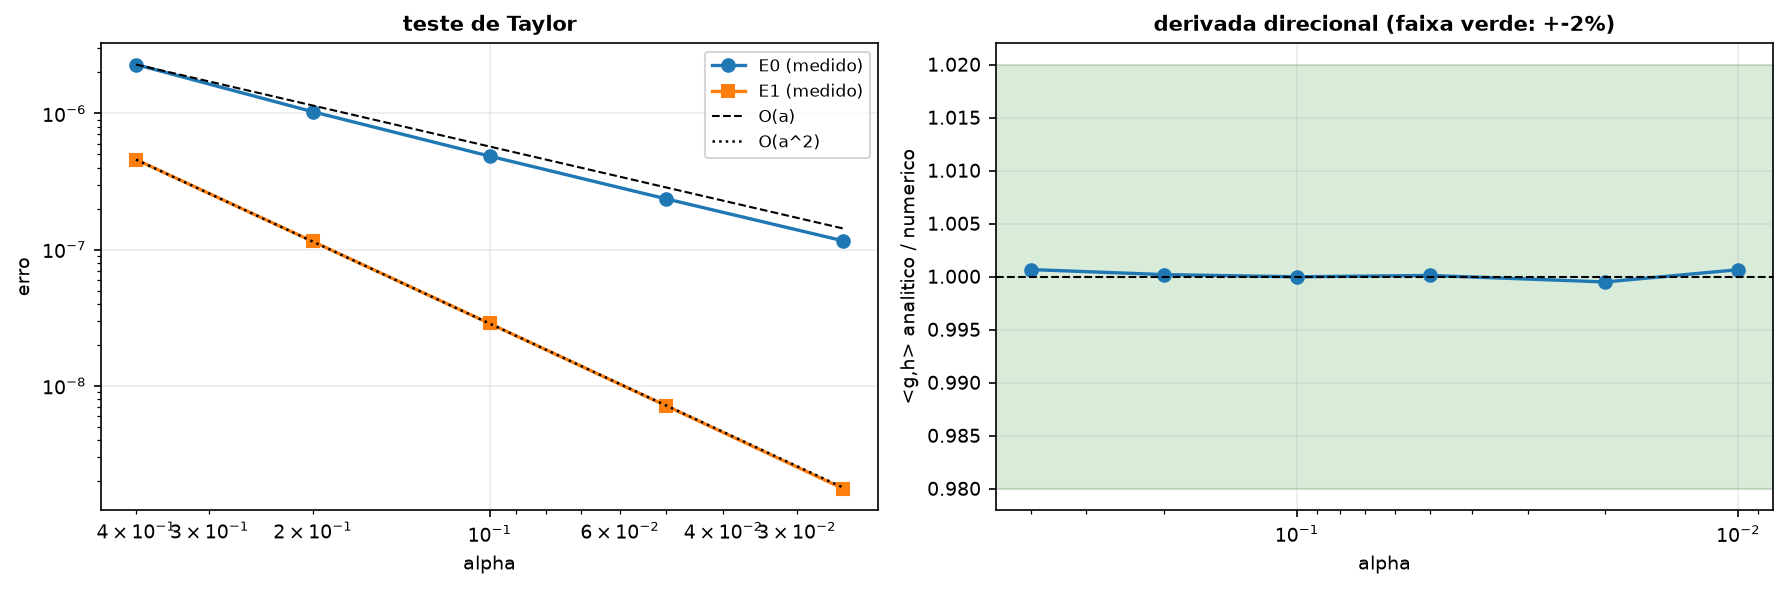
\includegraphics[width=0.96\textwidth]{../saidas/aula09/01_testes_de_gradiente.png}
\caption{Esquerda: teste de Taylor em log-log com as retas de refer\^encia de
inclina\c{c}\~ao 1 e 2. Direita: raz\~ao da derivada direcional, faixa verde de
$\pm 2\%$.}
\end{figure}

\begin{resumo}
\begin{itemize}[leftmargin=*, itemsep=1pt]
\item O teste do produto escalar verifica o \emph{adjunto} e fecha em
precis\~ao de m\'aquina; o de Taylor verifica a \emph{lineariza\c{c}\~ao}.
Passar num n\~ao implica passar no outro.
\item Vetores aleat\'orios s\~ao certos no teste do produto escalar e errados
no direcional (onde a dire\c{c}\~ao deve ser suave).
\item Refinar $\Delta t,\Delta h$ separa discrep\^ancia cont\'inuo/discreto
(encolhe) de \emph{bug} (n\~ao encolhe).
\item $\nabla_{\mvec}J = E^{T}\nabla_{\tilde{\mvec}}J$ para todo
pr\'e-processamento linear $E$ --- e $E^{T}$ de uma replica\c{c}\~ao \'e uma
soma, n\~ao um recorte.
\end{itemize}
\end{resumo}

\begin{exercicio}[Problemas]
\begin{enumerate}[leftmargin=*, itemsep=2pt]
\item Mostre que, se o operador ``direto'' implementado \'e $A$ e o
``adjunto'' implementado \'e $B \ne A^{*}$, o teste de Taylor ainda pode
passar com raz\~ao $1$ para uma dire\c{c}\~ao particular $\mathbf{h}$. Qual
propriedade de $\mathbf{h}$ torna isso poss\'ivel, e por que o teste do
produto escalar com vetores aleat\'orios n\~ao tem esse ponto cego?
\item Um c\'odigo aplica suaviza\c{c}\~ao gaussiana $S$ ao modelo antes de
propagar, e aplica $S$ tamb\'em ao gradiente. Isso est\'a certo? Sob qual
condi\c{c}\~ao?
\item O teste direcional d\'a raz\~ao $0{,}5000$ em todos os $\alpha$. Aponte
os dois \emph{bugs} mais prov\'aveis.
\end{enumerate}
\textbf{Respostas.} (1) Se $\mathbf{h}$ pertencer ao subespa\c{c}o em que
$B$ e $A^{*}$ coincidem --- t\'ipico quando o erro est\'a confinado a uma
regi\~ao (bordas, moldura) e $\mathbf{h}$ tem pouca energia ali. Um vetor
aleat\'orio tem componente em todos os modos com probabilidade 1, e por isso
n\~ao tem esse ponto cego. (2) Certo \emph{porque} o n\'ucleo gaussiano \'e
sim\'etrico, logo $S^{T} = S$; se o filtro fosse assim\'etrico (causal, por
exemplo) seria errado. Aplicar por acaso a opera\c{c}\~ao certa n\~ao \'e o
mesmo que aplicar o adjunto. (3) A derivada num\'erica, no denominador da
raz\~ao, saiu $2\times$ maior do que deveria: ou a diferen\c{c}a centrada foi dividida por $\alpha$ em vez de
$2\alpha$, ou o $J$ avaliado \'e $\norm{r}^{2}$ enquanto o gradiente foi
derivado de $\tfrac12\norm{r}^{2}$. (Os erros opostos dariam raz\~ao $2$.)
\end{exercicio}

% =====================================================================
\chapter{Otimiza\c{c}\~ao de segunda ordem e a Hessiana}
\label{cap:otimizacao}

\begin{ideia}
A Hessiana de FWI n\~ao pode ser formada, mas pode ser \emph{aplicada} a um
vetor pelo custo de duas modelagens adicionais. Isso basta para m\'etodos de
Newton truncado --- e, de quebra, d\'a a ferramenta quantitativa para
an\'alise de resolu\c{c}\~ao e para diagnosticar \emph{crosstalk}.
\end{ideia}

\begin{matematica}[m\'etodos de Krylov e por que ``aplicar'' basta]
\textbf{A observa\c{c}\~ao central.} Para resolver $H\,\delta = -\mathbf{g}$,
o m\'etodo dos gradientes conjugados nunca acessa $H$ elemento a elemento:
ele s\'o precisa de produtos $H\mathbf{v}$. O mesmo vale para GMRES,
Lanczos, e para estimativa de autovalores.

Formalmente, ap\'os $k$ itera\c{c}\~oes o CG minimiza a forma quadr\'atica
sobre o \textbf{subespa\c{c}o de Krylov}
\[
\mathcal{K}_k = \operatorname{span}\{\mathbf{g},\,H\mathbf{g},\,
H^{2}\mathbf{g},\dots,H^{k-1}\mathbf{g}\},
\]
que \'e constru\'ido apenas com aplica\c{c}\~oes sucessivas.

\textbf{Por que isso muda tudo em FWI.} $H$ tem $N^{2} \sim 10^{12}$
entradas --- imposs\'ivel. Mas $H\mathbf{v}$, como veremos, custa duas
modelagens. Com 5 a 15 itera\c{c}\~oes de CG por passo de Newton, isso \'e
compar\'avel ao custo de algumas itera\c{c}\~oes de l-BFGS --- e entrega
curvatura \emph{exata} em vez de estimada por hist\'orico.

\textbf{Truncamento e curvatura negativa.} Como $J$ n\~ao \'e convexa, $H$
pode ter autovalores negativos, e o CG falha nesse caso. Duas sa\'idas
padr\~ao: parar o CG assim que detectar
$\mathbf{v}^{T}H\mathbf{v} \le 0$ (e usar a dire\c{c}\~ao acumulada at\'e
ali, que ainda \'e de descida); ou usar a Hessiana de Gauss--Newton, que \'e
semidefinida positiva por constru\c{c}\~ao. O primeiro \'e ``Newton truncado'';
o segundo, ``Gauss--Newton truncado''.
\end{matematica}

\section{Estrutura da Hessiana}

Com $J = \tfrac12\norm{\mathbf{r}(\mvec)}^{2}$ e $J' = \partial\mathbf{r}/
\partial\mvec = F'$:
\begin{equation}
\mathbf{g} = F'^{*}\mathbf{r},
\qquad
H = \underbrace{F'^{*}F'}_{H_1 \;=\; H_{\text{GN}}}
  \;+\; \underbrace{\sum_i r_i\,\nabla^{2} r_i}_{H_2} .
\label{eq:hess3}
\end{equation}

\begin{teoria}[O que cada bloco significa fisicamente]
\textbf{$H_1 = F'^{*}F'$ (Gauss--Newton).} \'E o operador
\emph{migra\c{c}\~ao $\circ$ modelagem de Born}. Na diagonal, a
\textbf{ilumina\c{c}\~ao} de cada ponto; fora da diagonal, o quanto uma
perturba\c{c}\~ao num ponto \emph{imita} o efeito de uma perturba\c{c}\~ao em
outro --- ou seja, a \textbf{ambiguidade geom\'etrica} do experimento. Em
multipar\^ametro, os blocos fora da diagonal entre par\^ametros s\~ao
literalmente o \emph{crosstalk} (Cap.~\ref{cap:limites}).

Inverter $H_1$ corrige dois defeitos de uma vez: reequilibra a ilumina\c{c}\~ao
(diagonal) e \textbf{remove o desfoque} da imagem (fora da diagonal) --- \'e por isso
que Gauss--Newton produz modelos visivelmente mais n\'itidos que gradiente
puro, e n\~ao apenas mais r\'apidos.

\textbf{$H_2$ (termo de segunda ordem).} Cont\'em a informa\c{c}\~ao sobre
\textbf{espalhamento m\'ultiplo}: \'e o que distingue ``uma reflex\~ao de
segunda ordem'' de ``uma interface nova mais profunda''. Ele \'e pequeno
quando os res\'iduos s\~ao pequenos (por isso Gauss--Newton fica bom perto da
converg\^encia) e \emph{n\~ao} \'e pequeno no in\'icio, nem em presen\c{c}a de
m\'ultiplas fortes --- onde justamente ele seria mais \'util. Ignor\'a-lo \'e
defens\'avel; ignorar que se ignorou, n\~ao.
\end{teoria}

\section{Produto Hessiana--vetor pelo adjunto de segunda ordem}

\begin{derivacao}[Quatro propaga\c{c}\~oes, e o gradiente j\'a pagou duas]
Aplicar $H$ a uma dire\c{c}\~ao $\delta m$ equivale a derivar o gradiente na
dire\c{c}\~ao $\delta m$. Diferenciando o sistema
(estado, adjunto, gradiente) obt\'em-se quatro problemas em cascata:

\begin{enumerate}[leftmargin=*, itemsep=1pt]
\item \textbf{Estado}: $\mathcal{A}(m)p = s$ \hfill (j\'a calculado para
$\mathbf{g}$)
\item \textbf{Adjunto}: $\mathcal{A}^{*}\lambda = -R^{*}\mathbf{r}$
\hfill (j\'a calculado para $\mathbf{g}$)
\item \textbf{Tangente linear} (Born): $\mathcal{A}(m)\,\delta p
 = -\,\delta m\,\partial_{tt}p$ \hfill (\emph{nova})
\item \textbf{Adjunto de segunda ordem}:
 $\mathcal{A}^{*}\,\delta\lambda = -R^{*}R\,\delta p
  \;-\;\delta m\,\partial_{tt}\lambda$ \hfill (\emph{nova})
\end{enumerate}

e ent\~ao
\begin{equation}
\bigl[H\,\delta m\bigr](\mathbf{x})
 = \int_0^T \Bigl[\lambda\,\partial_{tt}\delta p
   + \delta\lambda\,\partial_{tt}p\Bigr]\dd t .
\end{equation}

O primeiro termo do lado direito de (4), correlacionado com $\partial_{tt}p$,
gera $H_1 = F'^{*}F'$. Os outros dois --- o termo $-\delta m\,\partial_{tt}\lambda$
em (4) e a parcela $\lambda\,\partial_{tt}\delta p$ da integral --- cont\^em o
campo adjunto $\lambda$, proporcional ao res\'iduo, e formam $H_2$.
\textbf{Omitir os dois produz exatamente $H_{\text{GN}}$}; omitir s\'o o de (4)
\emph{n\~ao} --- a parcela $\lambda\,\partial_{tt}\delta p$ continua l\'a. \'E
uma diferen\c{c}a de duas linhas de c\'odigo, conveniente e tamb\'em fonte de
confus\~ao na literatura.

\textbf{Custo:} 2 propaga\c{c}\~oes adicionais por produto, por tiro. Com
$k$ itera\c{c}\~oes de CG por passo de Newton, o passo custa
$\sim 2(1+k)$ propaga\c{c}\~oes por tiro.
\end{derivacao}

\section{Fun\c{c}\~ao de espalhamento de ponto e resolu\c{c}\~ao}

\begin{teoria}[Medindo resolu\c{c}\~ao sem conhecer a resposta]
Aplique $H_{\text{GN}}$ a uma perturba\c{c}\~ao pontual $\delta_{\mathbf{x}_0}$:
o resultado $H_{\text{GN}}\delta_{\mathbf{x}_0}$ \'e a coluna de
$H_{\text{GN}}$ em $\mathbf{x}_0$, conhecida como \textbf{fun\c{c}\~ao de
espalhamento de ponto} (PSF).

Ela responde, quantitativamente: \emph{se houvesse uma anomalia pontual aqui,
como ela apareceria na invers\~ao linearizada?} A largura da PSF \'e a
resolu\c{c}\~ao local; a sua orienta\c{c}\~ao revela a dire\c{c}\~ao
preferencial de ilumina\c{c}\~ao; a sua amplitude revela zonas cegas.

Tr\^es propriedades tornam a PSF a ferramenta certa:
\begin{itemize}[leftmargin=*, itemsep=1pt]
\item \'e calcul\'avel com o \emph{modelo estimado}, sem conhecer a verdade ---
portanto serve em dado real;
\item respeita a f\'isica e a geometria reais (ao contr\'ario de testes de
``tabuleiro de xadrez'', que dependem do padr\~ao escolhido);
\item custa 2 propaga\c{c}\~oes por tiro por ponto avaliado, o que permite
mapear a resolu\c{c}\~ao em alguns pontos-chave a custo modesto.
\end{itemize}

Ela \'e tamb\'em a confirma\c{c}\~ao emp\'irica da an\'alise de
§\ref{sec:cobertura}: a transformada de Fourier da PSF \'e, essencialmente, a
cobertura de $\mathbf{k}_m$ naquele ponto.
\end{teoria}

\section{Pr\'e-condicionamento, revisitado}

O pseudo-Hessiano de Shin \emph{et al.} aproxima
$\operatorname{diag}(H_{\text{GN}})$ pela energia do campo direto:
\begin{equation}
P^{-1}_{ii} \approx \int_0^T\bigl[\partial_{tt}p(\mathbf{x}_i,t)\bigr]^{2}\dd t
 + \epsilon .
\end{equation}

\begin{atencao}[O que essa aproxima\c{c}\~ao descarta, exatamente]
Duas coisas, e vale saber quais. \textbf{(1)} Os termos fora da diagonal ---
isto \'e, o desfoque; a corre\c{c}\~ao \'e s\'o de ilumina\c{c}\~ao, n\~ao de
resolu\c{c}\~ao. \textbf{(2)} A propaga\c{c}\~ao de cada ponto \emph{at\'e os
receptores}: a diagonal exata de $F'^{*}F'$ envolve tamb\'em
$\abs{G(\mathbf{x}_r,\mathbf{x})}^{2}$, que o pseudo-Hessiano ignora.

Ainda assim \'e o pr\'e-condicionador padr\~ao, porque custa zero (o campo
direto j\'a est\'a l\'a) e captura o efeito dominante, que \'e o decaimento
geom\'etrico com a profundidade. Medido no curso: raz\~ao de ilumina\c{c}\~ao
raso/profundo de $181\times$.
\end{atencao}

Efeito medido (correla\c{c}\~ao do gradiente com a perturba\c{c}\~ao
verdadeira): bruto $+0{,}0390$; mascarado $+0{,}0830$; mascarado e suavizado
$+0{,}0842$; com compensa\c{c}\~ao de profundidade $+0{,}0898$. Os valores
absolutos s\~ao baixos porque um gradiente \emph{n\~ao \'e} o modelo --- ele
\'e $F'^{*}r$, espalhado nas is\'ocronas, e s\'o $H^{-1}F'^{*}r$ seria uma
estimativa do modelo. O que importa \'e a raz\~ao relativa: o tratamento mais
que dobra a correla\c{c}\~ao.

\section{Otimiza\c{c}\~ao estoc\'astica e codifica\c{c}\~ao de fontes}

\begin{teoria}[Dois jeitos de n\~ao pagar por todos os tiros]
\textbf{Subconjunto aleat\'orio.} Sorteie $n_{\text{sub}} \ll n_s$ tiros por
itera\c{c}\~ao. O gradiente resultante, reescalado por $n_s/n_{\text{sub}}$,
\'e um \emph{estimador n\~ao viesado} do gradiente completo:
$\mathbb{E}[\mathbf{g}_{\text{sub}}] = \mathbf{g}$. A
teoria de aproxima\c{c}\~ao estoc\'astica garante converg\^encia sob passos
decrescentes; na pr\'atica usa-se $n_{\text{sub}}$ crescente ao longo das
itera\c{c}\~oes (\emph{sample size scheduling}), come\c{c}ando barato e
terminando preciso.

\textbf{Codifica\c{c}\~ao de fontes (\emph{source encoding}; Krebs \emph{et
al.}, 2009).} Some todos os
tiros em um \'unico ``supertiro'', cada um multiplicado por um peso aleat\'orio
$\varepsilon_s$ (sinal $\pm1$, ou fase aleat\'oria). Como
$\mathbb{E}[\varepsilon_s\varepsilon_{s'}] = \delta_{ss'}$, os termos cruzados
t\^em m\'edia zero e o gradiente do supertiro \'e n\~ao viesado. O custo cai
por um fator $n_s$.

\textbf{O pre\c{c}o:} no subconjunto, ru\'ido de amostragem (os tiros que
ficaram de fora); na codifica\c{c}\~ao, termos cruzados que n\~ao s\~ao zero em
cada realiza\c{c}\~ao --- ru\'ido de \emph{crosstalk}. Nos dois casos ele decai
como $1/\sqrt{n_{\text{real}}}$. E a codifica\c{c}\~ao exige que todos os tiros
compartilhem a mesma geometria de receptores (aquisi\c{c}\~ao fixa), o que
exclui boa parte do dado marinho rebocado sem re-datuma\c{c}\~ao.
\end{teoria}

\begin{resumo}
\begin{itemize}[leftmargin=*, itemsep=1pt]
\item $H = F'^{*}F' + \sum_i r_i\nabla^{2}r_i$: o primeiro bloco \'e
ilumina\c{c}\~ao $+$ desfoque, o segundo \'e espalhamento m\'ultiplo.
\item $H\mathbf{v}$ custa 2 propaga\c{c}\~oes extras (adjunto de segunda
ordem); com Krylov, isso basta para Newton truncado.
\item A PSF mede resolu\c{c}\~ao local sem conhecer a verdade, e \'e a
verifica\c{c}\~ao emp\'irica da cobertura de $\mathbf{k}_m$.
\item Estimadores estoc\'asticos s\~ao n\~ao viesados; o pre\c{c}o \'e
ru\'ido de \emph{crosstalk} $\propto 1/\sqrt{n_{\text{real}}}$.
\end{itemize}
\end{resumo}

\begin{exercicio}[Problemas]
\begin{enumerate}[leftmargin=*, itemsep=2pt]
\item Mostre que $H_{\text{GN}} = F'^{*}F'$ \'e semidefinida positiva, e
explique por que isso garante que a dire\c{c}\~ao de Gauss--Newton seja de
descida (quando o sistema \'e resolvido exatamente).
\item Estime o custo, em modelagens por tiro, de um passo de Gauss--Newton
truncado com 8 itera\c{c}\~oes de CG, e compare com 8 itera\c{c}\~oes de
l-BFGS supondo busca linear de 2 avalia\c{c}\~oes.
\item A PSF num ponto profundo sai alongada na horizontal. Que propriedade da
aquisi\c{c}\~ao isso revela, e por que \eqref{eq:km} j\'a permitia prev\^e-lo?
\item Com codifica\c{c}\~ao de fontes, o ru\'ido de \emph{crosstalk} decai como
$1/\sqrt{n_{\text{real}}}$. Quantas realiza\c{c}\~oes seriam necess\'arias para
que ele caia $20$\,dB abaixo do n\'ivel inicial? Compare esse custo com o de
inverter os tiros individualmente.
\end{enumerate}
\textbf{Respostas.} (1)
$\mathbf{v}^{T}F'^{*}F'\mathbf{v} = \norm{F'\mathbf{v}}^{2}\ge0$; com
$H_{\text{GN}}$ positiva definida,
$\inner{\mathbf{g}}{-H_{\text{GN}}^{-1}\mathbf{g}} < 0$. (2) Gauss--Newton
truncado: $2$ (gradiente) $+\,2\times8$ (produtos $H\mathbf{v}$) $= 18$
modelagens por tiro, mais a busca linear, para \emph{um} passo; l-BFGS:
$8\times(2+2) = 32$ para 8 passos, busca linear j\'a inclu\'ida. A
compara\c{c}\~ao justa depende de quantos passos de l-BFGS equivalem a um de
Newton --- que \'e precisamente o que se mede, e depende do condicionamento. (3) Ilumina\c{c}\~ao
predominantemente vertical, isto \'e, \^angulos de espalhamento concentrados
perto de $\pi$: por \eqref{eq:km} os $\mathbf{k}_m$ dispon\'iveis apontam quase
todos na vertical, e a resolu\c{c}\~ao horizontal fica pobre --- a PSF alonga
na dire\c{c}\~ao \emph{n\~ao} coberta. (4) $20$\,dB \'e um fator 10 em
amplitude, logo $n_{\text{real}} = 100$. Isso s\'o compensa se
$n_s \gg 100$; abaixo disso, inverter os tiros separadamente \'e mais barato
e sem vi\'es.
\end{exercicio}

% =====================================================================
\chapter{Fluxo completo, escalabilidade e reprodutibilidade}
\label{cap:completa}

\begin{ideia}
Em escala de produ\c{c}\~ao, as decis\~oes que determinam o resultado s\~ao de
engenharia: qual dom\'inio, quais frequ\^encias, quanta mem\'oria, qual
paralelismo. Todas t\^em uma justificativa te\'orica --- e a mais elegante
delas sai diretamente da cobertura de n\'umero de onda do
Cap\'itulo~\ref{cap:oque}.
\end{ideia}

\begin{matematica}[custo de resolver a mesma EDP de dois jeitos]
A escolha entre dom\'inio do tempo e da frequ\^encia n\~ao \'e de gosto: \'e
uma conta de \'algebra linear.

\textbf{No tempo}, a marcha \'e \emph{expl\'icita}: cada passo \'e um produto
matriz esparsa--vetor, $\mathcal{O}(N)$ opera\c{c}\~oes, sem resolver sistema
algum. O custo total \'e $\mathcal{O}(n_t N)$ por tiro, e a mem\'oria \'e
$\mathcal{O}(N)$ --- mais o \emph{checkpointing}.

\textbf{Na frequ\^encia}, cada $\omega$ exige resolver
$\mathcal{A}_\omega \hat u = \hat s$, um sistema linear esparso. Com
fatora\c{c}\~ao direta (LU), paga-se caro \emph{uma vez} e cada tiro adicional
custa apenas uma substitui\c{c}\~ao, proporcional ao tamanho dos fatores.
\textbf{Com muitos tiros, a fatora\c{c}\~ao rateada por tiro tende a zero}, e
sobra s\'o a substitui\c{c}\~ao. Essa \'e a vantagem estrutural do
dom\'inio da frequ\^encia.

\textbf{Por que ela desaparece em 3D.} O custo e a mem\'oria de uma
fatora\c{c}\~ao esparsa dependem do \emph{preenchimento} (\emph{fill-in}) dos
fatores, que por sua vez depende da estrutura do grafo da matriz. Em 2D, uma
boa ordena\c{c}\~ao (dissec\c{c}\~ao aninhada) mant\'em o preenchimento
modesto. Em 3D o separador de um cubo $n^{3}$ \'e uma \emph{superf\'icie}
$n^{2}$, e a mem\'oria dos fatores cresce como $\mathcal{O}(n^{4})$: para
$n = 500$ isso \'e muitos terabytes.

Da\'i a divis\~ao pr\'atica: frequ\^encia em 2D com muitos tiros, tempo em 3D.
\end{matematica}

\section{Dom\'inio do tempo \emph{versus} dom\'inio da frequ\^encia}

\begin{center}
\begin{tabular}{@{}lp{4.6cm}p{4.9cm}@{}}
\toprule
 & \textbf{Tempo} & \textbf{Frequ\^encia} \\
\midrule
Como resolve & marcha expl\'icita em $n_t$ passos
  & sistema linear esparso por $\omega$ \\
Custo por tiro & $\mathcal{O}(n_t N)$ & fatora\c{c}\~ao LU reaproveitada por
  \emph{todos} os tiros \\
Mem\'oria & campo $+$ \emph{checkpointing} & fatores LU --- cresce muito
  r\'apido em 3D \\
Multiescala & filtrar o dado & \textbf{escolher as frequ\^encias} \\
Atenua\c{c}\~ao & operadores fracion\'arios ou SLS & trivial: $Q$ complexo
  na velocidade \\
Onde domina & 3D & 2D com muitos tiros \\
\bottomrule
\end{tabular}
\end{center}

\begin{teoria}[Por que poucas frequ\^encias discretas podem bastar]
Esta \'e uma das consequ\^encias mais bonitas de \eqref{eq:km}, e a
justificativa da estrat\'egia de Sirgue \& Pratt.

Um \emph{\'unico} $\omega$, combinado com \emph{toda} a faixa de \^angulos de
espalhamento dispon\'ivel $[\theta_{\min},\theta_{\max}]$, j\'a cobre uma
\textbf{faixa cont\'inua} de n\'umeros de onda:
\[
\abs{\mathbf{k}_m} \in
\left[\frac{2\omega}{c}\sin\frac{\theta_{\min}}{2},\;
      \frac{2\omega}{c}\sin\frac{\theta_{\max}}{2}\right].
\]
H\'a, portanto, \textbf{redund\^ancia} entre frequ\^encia e \^angulo: um dado
$\abs{\mathbf{k}_m}$ pode ser alcan\c{c}ado por muitos pares
$(\omega,\theta)$. Inverter todas as frequ\^encias \'e desperdi\c{c}ar essa
redund\^ancia.

A estrat\'egia \'e escolher $\omega_1 < \omega_2 < \dots$ de modo que as
faixas cobertas se \emph{encostem} sem lacuna:
\[
\frac{2\omega_{j+1}}{c}\sin\frac{\theta_{\min}}{2}
 \;\le\; \frac{2\omega_{j}}{c}\sin\frac{\theta_{\max}}{2}
\quad\Longrightarrow\quad
\frac{\omega_{j+1}}{\omega_j} \le
\frac{\sin(\theta_{\max}/2)}{\sin(\theta_{\min}/2)} .
\]
O espa\c{c}amento \'e \textbf{geom\'etrico}, e o passo depende s\'o da
\emph{abertura angular}. Aquisi\c{c}\~ao de abertura larga permite passos
maiores --- menos frequ\^encias, menos custo. \'E o mesmo compromisso
frequ\^encia$\leftrightarrow$abertura de §\ref{sec:cobertura}, agora como
regra de projeto.
\end{teoria}

\section{O fluxo, e a ordem que n\~ao muda}

\begin{lstlisting}
# --- antes de qualquer inversao ---
1. preparar dado (direta, multiplas, 2.5D se for o caso, wavelet)
2. modelo inicial  +  caixa de velocidades fisicamente plausivel
3. dimensionar dh, dt, moldura                      (Caps. 3, 4)
4. TESTE DO PRODUTO ESCALAR no par Born/migracao    (Cap. 7)
5. TESTE DE TAYLOR no gradiente                     (Cap. 7)

# --- multiescala ---
6. para cada banda (ou grupo de frequencias):
       reestimar a wavelet por projecao variavel    (Cap. 2)
       reiniciar o historico do quase-Newton
       iterar:  gradiente -> precondicionar -> direcao -> busca
                -> projetar na caixa                (Caps. 6, 8, 10)

# --- depois ---
7. PSF em pontos-chave: mapa de resolucao           (Cap. 8)
8. analise de residuo; relatorio com erro INICIAL   (Cap. 12)
\end{lstlisting}

\section{Resultados medidos, e o fracasso que n\~ao parece fracasso}

Estudo de robustez do curso: quatro modelos iniciais, monoescala (25\,Hz)
contra multiescala (5/12/25\,Hz), mesmo n\'umero total de itera\c{c}\~oes.

\begin{center}
\begin{tabular}{@{}lrrrr@{}}
\toprule
\textbf{Modelo inicial} & \textbf{erro ini.} & \textbf{mono} & \textbf{multi}
& \textbf{vantagem} \\
\midrule
linear suave           & 7{,}96\%  & 7{,}34\%  & \textbf{7{,}07\%}  & $+0{,}27$ pp \\
linear lento (viesado) & 16{,}68\% & \textbf{17{,}57\%} & \textbf{17{,}34\%} & $+0{,}24$ pp \\
constante              & 16{,}32\% & 16{,}10\% & 16{,}06\% & $+0{,}04$ pp \\
suavizado forte        & 4{,}95\%  & 4{,}01\%  & \textbf{3{,}70\%}  & $+0{,}31$ pp \\
\bottomrule
\end{tabular}
\end{center}

\begin{armadilha}[Leia a segunda linha]
Erro inicial $16{,}68\%$, erro final $17{,}57\%$: \textbf{a invers\~ao piorou o
modelo}, com $J$ caindo monotonicamente o tempo todo. Ela convergiu para um
m\'inimo local e, no caminho, destruiu informa\c{c}\~ao que j\'a se tinha.

Em termos da §\ref{sec:cobertura}: um erro de $\sim16\%$ com
$c\approx2300$\,m/s e percursos de 1--2\,km fica na borda ou fora do vale de
atra\c{c}\~ao \emph{j\'a a 5\,Hz} --- e a\'i nenhuma ordem de bandas resgata.
A vantagem da multiescala \emph{n\~ao} cresceu com a degrada\c{c}\~ao do
inicial, contrariando a expectativa comum, porque ela s\'o resgata o que a
banda mais baixa alcan\c{c}a.

\textbf{Nota metodol\'ogica:} sem reportar o erro inicial, essa linha seria
indistingu\'ivel de um sucesso.
\end{armadilha}

\section{Reprodutibilidade}

\begin{pratica}[O m\'inimo para que um resultado de FWI seja verific\'avel]
\begin{itemize}[leftmargin=*, itemsep=1pt]
\item \textbf{Modelo inicial}, com o seu erro relativo --- e como ele foi
obtido;
\item \textbf{banda por est\'agio}, tipo e ordem do filtro, e se ele foi
aplicado aos dois lados;
\item \textbf{discretiza\c{c}\~ao}: $\Delta h$, $\Delta t$, ordem, $G$
resultante, tipo e espessura da moldura;
\item \textbf{resultado do teste de gradiente}, com o n\'umero;
\item \textbf{regulariza\c{c}\~ao}: forma, peso, e \emph{como o peso foi
escolhido} (curva em L? erro de modelo? --- se foi o segundo, dizer);
\item \textbf{tratamento do gradiente}: m\'ascaras, suaviza\c{c}\~ao,
pr\'e-condicionador;
\item \textbf{crit\'erio de parada}, e n\'umero de modelagens gasto;
\item \textbf{curva de converg\^encia com eixo de custo}, perfis, mapa de
erro, e o \textbf{res\'iduo final} (n\~ao s\'o o valor de $J$).
\end{itemize}
Um trabalho que omite o erro do modelo inicial n\~ao permite avaliar se a
invers\~ao agregou alguma coisa.
\end{pratica}

\begin{resumo}
\begin{itemize}[leftmargin=*, itemsep=1pt]
\item Tempo escala bem em 3D; frequ\^encia amortiza a fatora\c{c}\~ao entre
tiros e domina em 2D --- o divisor de \'aguas \'e o preenchimento dos fatores.
\item Redund\^ancia entre $\omega$ e $\theta$ em \eqref{eq:km} justifica
inverter \emph{poucas} frequ\^encias, com espa\c{c}amento geom\'etrico ditado
pela abertura angular.
\item A ordem do fluxo \'e r\'igida em um ponto: verifica\c{c}\~ao de gradiente
antes da primeira invers\~ao.
\item Um relat\'orio sem o erro do modelo inicial n\~ao permite avaliar se a
invers\~ao agregou informa\c{c}\~ao --- e o estudo de robustez mostra um caso
em que ela \emph{destruiu}.
\end{itemize}
\end{resumo}

% =====================================================================
\chapter{Regulariza\c{c}\~ao, priors e infer\^encia}
\label{cap:regularizacao}

\begin{ideia}
Toda regulariza\c{c}\~ao \'e um prior disfar\c{c}ado, e reconhecer isso muda o
que se pode afirmar sobre o resultado. A formula\c{c}\~ao bayesiana d\'a, de
gra\c{c}a, a interpreta\c{c}\~ao dos pesos e uma estimativa de incerteza ---
v\'alida, e vale entender exatamente at\'e onde.
\end{ideia}

\begin{matematica}[Bayes, MAP e a aproxima\c{c}\~ao de Laplace]
\textbf{Bayes.} Com $\mvec$ os par\^ametros e $\mathbf{d}$ o dado,
\[
\underbrace{\pi(\mvec\mid\mathbf{d})}_{\text{posterior}}
 \;\propto\;
\underbrace{\pi(\mathbf{d}\mid\mvec)}_{\text{verossimilhan\c{c}a}}\;
\underbrace{\pi(\mvec)}_{\text{prior}} .
\]

\textbf{Verossimilhan\c{c}a gaussiana.} Se o ru\'ido \'e gaussiano de
covari\^ancia $C_d$,
$-\log\pi(\mathbf{d}\mid\mvec)
 = \tfrac12\norm{F(\mvec)-\mathbf{d}}^{2}_{C_d^{-1}} + \text{const}$,
onde $\norm{v}^{2}_{C_d^{-1}} = v^{T}C_d^{-1}v$. \textbf{O $L_2$ simples da
Parte II \'e o caso $C_d = \sigma^{2}I$}: ru\'ido branco, mesma
vari\^ancia em todo tra\c{c}o e todo instante --- hip\'otese quase nunca
verdadeira e quase nunca declarada.

\textbf{Prior gaussiano.} Com $\pi(\mvec) \propto
\exp[-\tfrac12\norm{\mvec-\mvec_{\text{pr}}}^{2}_{C_m^{-1}}]$,
\[
-\log\pi(\mvec\mid\mathbf{d})
 = \tfrac12\norm{F(\mvec)-\mathbf{d}}^{2}_{C_d^{-1}}
 + \tfrac12\norm{\mvec-\mvec_{\text{pr}}}^{2}_{C_m^{-1}} + \text{const}.
\]
Maximizar o posterior (estimativa \textbf{MAP}) \'e \emph{exatamente}
minimizar o funcional regularizado. Portanto:
\begin{center}
\emph{escolher $R$ e $\lambda$ \'e escolher um prior, queira-se ou n\~ao.}
\end{center}

\textbf{Aproxima\c{c}\~ao de Laplace.} Expandindo $-\log\pi$ em torno do MAP
at\'e segunda ordem, o posterior \'e aproximado por uma gaussiana com
\[
C_{\text{post}} \approx H_{\text{MAP}}^{-1},
\qquad
H_{\text{MAP}} = F'^{*}C_d^{-1}F' + C_m^{-1} + (\text{termo de 2\textsuperscript{a} ordem}).
\]
\textbf{A Hessiana \'e a covari\^ancia a posteriori inversa.} \'E a mesma
matriz do Cap\'itulo~\ref{cap:otimizacao}, agora com leitura estat\'istica:
dire\c{c}\~ao de autovalor grande = bem determinada; autovalor pequeno = o
dado n\~ao disse nada, e o prior \'e quem responde.
\end{matematica}

\section{Tradu\c{c}\~ao: regularizador $\leftrightarrow$ prior}

\begin{center}
\begin{tabular}{@{}p{4.3cm}p{5.2cm}p{5.3cm}@{}}
\toprule
\textbf{Regularizador} & \textbf{Prior equivalente} & \textbf{Afirma\c{c}\~ao
impl\'icita} \\
\midrule
$\tfrac{\lambda}{2}\norm{\mvec-\mvec_{\text{pr}}}^{2}$
  & gaussiano, $C_m^{-1} = \lambda I$
  & ``desvios do prior s\~ao pequenos e independentes'' \\
$\tfrac{\lambda}{2}\int\abs{\nabla m}^{2}$ (Tikhonov)
  & gaussiano com $C_m^{-1} = \lambda D^{T}D$
  & ``o modelo \'e suave'' \\
$\lambda\int\abs{\nabla m}$ (TV)
  & laplaciano nos gradientes
  & ``o modelo \'e constante por peda\c{c}os'' \\
caixa $v\in[v_{\min},v_{\max}]$
  & prior uniforme com suporte compacto
  & ``fora disso \'e imposs\'ivel'' \\
parada antecipada
  & prior impl\'icito, dependente do otimizador
  & --- (n\~ao control\'avel) \\
\bottomrule
\end{tabular}
\end{center}

\begin{armadilha}[A \'ultima linha \'e a mais perigosa]
Parada antecipada \emph{\'e} regulariza\c{c}\~ao: ela restringe a solu\c{c}\~ao
ao subespa\c{c}o de Krylov percorrido at\'e ali, tipicamente as
dire\c{c}\~oes de maior autovalor de $H$ --- isto \'e, as escalas grandes. O
efeito \'e real e frequentemente ben\'efico.

O problema \'e que esse prior \textbf{n\~ao \'e declar\'avel, n\~ao \'e
reprodut\'ivel e depende do otimizador}: trocar l-BFGS por gradiente
conjugado muda a regulariza\c{c}\~ao efetiva sem que ningu\'em anote. \'E a
raz\~ao pela qual o crit\'erio de parada deve entrar no relat\'orio junto com
$\lambda$.
\end{armadilha}

\section{A curva em L, e o resultado que contraria a expectativa}

Calibre $\lambda$ por $\lambda = \eta\,J_{\text{dados}}(\mvec_0)/R(\mvec_0)$
com $\eta\approx 0{,}02$, e refine pelo cotovelo da curva em L (ajuste
\emph{versus} penalidade, ambos em log).

\begin{figure}[htbp]
\centering
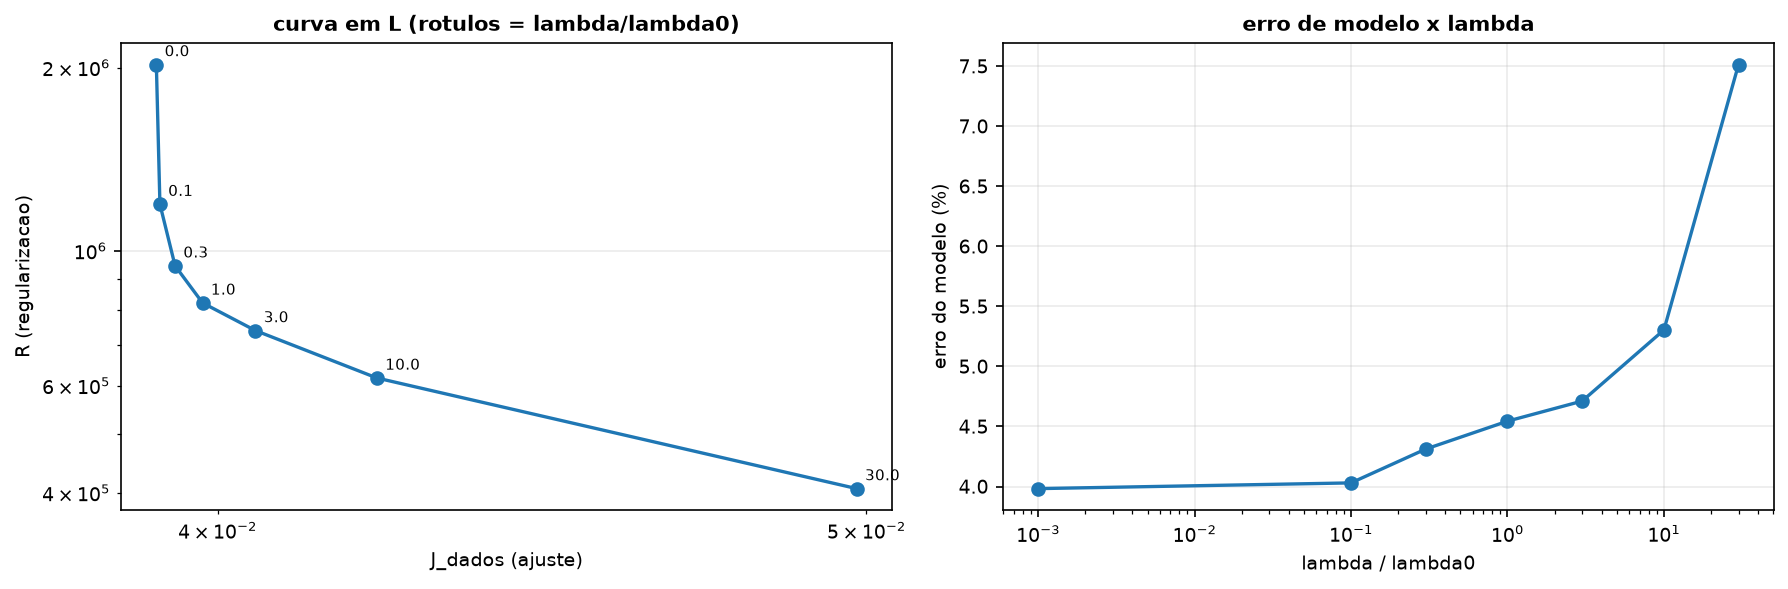
\includegraphics[width=0.78\textwidth]{../saidas/aula13/02_curva_em_L.png}
\caption{Curva em L medida no curso. O cotovelo \'e o ponto a partir do qual
se passa a pagar ajuste por suavidade.}
\end{figure}

Experimento do curso com rela\c{c}\~ao sinal/ru\'ido de 0\,dB:

\begin{center}
\begin{tabular}{@{}lrr@{}}
\toprule
\textbf{Variante} & \textbf{Erro final} & \textbf{Correla\c{c}\~ao} \\
\midrule
modelo inicial & 4{,}75\% & 0{,}9554 \\
sem regulariza\c{c}\~ao & 3{,}60\% & 0{,}9699 \\
Tikhonov & 4{,}42\% & 0{,}9595 \\
TV & 4{,}39\% & 0{,}9613 \\
\textbf{s\'o suaviza\c{c}\~ao do gradiente} & \textbf{3{,}56\%} & \textbf{0{,}9709} \\
\bottomrule
\end{tabular}
\end{center}

\begin{teoria}[A leitura bayesiana do resultado]
A regulariza\c{c}\~ao expl\'icita \emph{piorou}. Na linguagem deste
cap\'itulo: o prior estava \textbf{errado para este problema}.

O erro residual n\~ao era rugosidade --- era falta de \emph{contraste}, isto
\'e, amplitude insuficiente nos degraus. Um prior de suavidade penaliza
exatamente a quantidade que ainda faltava construir. Somando a isso os priors
\emph{impl\'icitos} j\'a presentes (modelo inicial suave, poucas
itera\c{c}\~oes, bandas baixas, suaviza\c{c}\~ao do gradiente), o posterior
ficou dominado pelo prior, e o dado deixou de mandar.

\textbf{Sobre-regulariza\c{c}\~ao \'e um diagn\'ostico, n\~ao uma
opini\~ao:} se afrouxar $\lambda$ melhora simultaneamente $J_{\text{dados}}$ e
o erro de modelo, o prior estava apertado demais.
\end{teoria}

\section{O que \'e honesto dizer sobre incerteza em FWI}

\begin{teoria}[A aproxima\c{c}\~ao de Laplace \'e local, e essa \'e a
limita\c{c}\~ao decisiva]
$C_{\text{post}} \approx H^{-1}$ descreve a curvatura em torno de \emph{um}
m\'inimo. Ela quantifica corretamente:
\begin{itemize}[leftmargin=*, itemsep=1pt]
\item quais dire\c{c}\~oes do modelo o dado restringe e quais n\~ao ---
autovalores pequenos de $H$ s\~ao o espa\c{c}o nulo pr\'atico;
\item como o ru\'ido do dado se propaga para o modelo, \emph{dado} que
estamos na bacia certa.
\end{itemize}

E \textbf{n\~ao} quantifica, de forma nenhuma:
\begin{itemize}[leftmargin=*, itemsep=1pt]
\item a probabilidade de estarmos na bacia \emph{errada} --- que \'e, na
pr\'atica, a maior fonte de erro em FWI;
\item erro de modelagem (f\'isica faltante), que \'e determin\'istico e
coerente, n\~ao ru\'ido;
\item erro na ondaleta da fonte, a menos que ela entre como par\^ametro.
\end{itemize}

Uma barra de erro derivada de $H^{-1}$ \'e portanto uma afirma\c{c}\~ao
\textbf{condicional}: ``supondo que o m\'inimo encontrado \'e o certo, e que a
f\'isica est\'a certa, a incerteza \'e esta''. Report\'a-la sem esse
condicional \'e enganoso, e \'e comum.
\end{teoria}

\begin{pratica}[O que se faz na pr\'atica, em ordem de custo]
\begin{enumerate}[leftmargin=*, itemsep=1pt]
\item \textbf{PSF} em pontos-chave (Cap.~\ref{cap:otimizacao}): resolu\c{c}\~ao
local, barato, e n\~ao exige conhecer a verdade.
\item \textbf{Autovetores dominantes de $H$} por Lanczos ou SVD aleatorizada,
usando os produtos $H\mathbf{v}$ do adjunto de segunda ordem. Em problemas de
FWI o espectro de $F'^{*}C_d^{-1}F'$ decai r\'apido, de modo que uma
aproxima\c{c}\~ao de posto baixo captura bem $C_{\text{post}}$ --- \'e o que
torna a UQ bayesiana vi\'avel apesar do tamanho.
\item \textbf{Ensemble de invers\~oes}: varie modelo inicial, banda inicial,
$\lambda$, subconjunto de tiros. A dispers\~ao entre os resultados amostra
justamente o que $H^{-1}$ \emph{n\~ao} captura --- inclusive bacias
diferentes. \'E caro e \'e o \'unico diagn\'ostico honesto sobre m\'inimos
locais.
\item \textbf{Passeios pelo espa\c{c}o nulo}: perturbe o modelo final ao longo
de dire\c{c}\~oes de autovalor pequeno e verifique que o dado praticamente
n\~ao muda. Isso exibe \emph{explicitamente} modelos alternativos que
explicam o dado igualmente bem.
\item \textbf{MCMC} em FWI de escala real: invi\'avel hoje. Resultados
existentes s\~ao 2D, de dimens\~ao modesta --- de dezenas a algumas dezenas de
milhares de par\^ametros, como na FWI el\'astica por Monte Carlo Hamiltoniano
de Gebraad \emph{et al.} (2020) --- ou usam substitutos (\emph{surrogates}). Trate afirma\c{c}\~oes de ``UQ completa'' em 3D com
ceticismo, e pergunte qual era a dimens\~ao efetiva.
\end{enumerate}
\end{pratica}

\begin{resumo}
\begin{itemize}[leftmargin=*, itemsep=1pt]
\item MAP $=$ m\'inimos quadrados regularizados: escolher $R$ e $\lambda$ \'e
escolher um prior.
\item $C_{\text{post}} \approx H^{-1}$ --- a Hessiana da otimiza\c{c}\~ao \'e a
precis\~ao a posteriori.
\item Priors impl\'icitos (parada antecipada, modelo inicial, multiescala)
frequentemente dominam o expl\'icito.
\item Incerteza de Laplace \'e condicional \`a bacia e \`a f\'isica; o \'unico
diagn\'ostico honesto sobre m\'inimos locais \'e o ensemble.
\end{itemize}
\end{resumo}

% =====================================================================
\part*{\centering\color{azulfwi} Parte III --- Os limites}
\addcontentsline{toc}{part}{Parte III --- Os limites}

\chapter{Multipar\^ametro, atenua\c{c}\~ao e anisotropia}
\label{cap:limites}

\begin{ideia}
Em invers\~ao multipar\^ametro, o obst\'aculo n\~ao \'e calcular gradientes ---
isso custa o mesmo. O obst\'aculo \'e que os blocos fora da diagonal da
Hessiana n\~ao s\~ao desprez\'iveis, e o algoritmo atribui ao par\^ametro
errado um efeito que pertencia a outro.
\end{ideia}

\section{\emph{Crosstalk}, definido com precis\~ao}

\begin{teoria}[O que \emph{crosstalk} \emph{\'e}]
Com dois par\^ametros $(p_1,p_2)$, a Hessiana de Gauss--Newton tem estrutura
de blocos
\[
H_{\text{GN}} =
\begin{pmatrix}
F_1'^{*}F_1' & F_1'^{*}F_2' \\[2pt]
F_2'^{*}F_1' & F_2'^{*}F_2'
\end{pmatrix},
\]
com $F_k' = \partial F/\partial p_k$. O passo de Gauss--Newton exige inverter
essa matriz \emph{inteira}.

O gradiente, por si, ignora os blocos fora da diagonal: ele atribui a $p_1$
toda a varia\c{c}\~ao de dado compat\'ivel com $F_1'$, inclusive a parcela
causada de fato por $p_2$. \textbf{\emph{Crosstalk} \'e precisamente a
magnitude relativa de $F_1'^{*}F_2'$} --- e o produto interno
$\inner{F_1'\delta p_1}{F_2'\delta p_2}$ mede o quanto os dois par\^ametros
produzem dado parecido.

\textbf{Consequ\^encias, todas verific\'aveis:}
\begin{itemize}[leftmargin=*, itemsep=1pt]
\item se os padr\~oes de radia\c{c}\~ao dos dois par\^ametros forem
\emph{ortogonais} na faixa angular \emph{iluminada}, o bloco cruzado \'e
pequeno e o \emph{crosstalk} \'e baixo;
\item se a aquisi\c{c}\~ao n\~ao cobrir os \^angulos que separam os dois,
nenhum algoritmo os separa --- \'e limita\c{c}\~ao de \emph{dado}, n\~ao de
m\'etodo;
\item reparametrizar (§\ref{sec:param}) \'e literalmente aplicar uma
congru\^encia $\Phi'^{T}H\Phi'$ escolhida para reduzir os blocos cruzados.
\end{itemize}
\end{teoria}

Do Cap\'itulo~\ref{cap:fisica}, para o caso ac\'ustico com densidade:
\[
f(\theta) \propto
 \frac{\delta I_p}{I_p}(\cos\theta - 1)
 - \frac{\delta c}{c}(1+\cos\theta),
\]
padr\~oes complementares --- \'e \emph{por isso} que $(I_p,c)$ tem menos
\emph{crosstalk} que $(\kappa,\rho)$. A escolha de parametriza\c{c}\~ao \'e a
principal ferramenta contra \emph{crosstalk}, e ela \'e gr\'atis.

\begin{atencao}[A ambiguidade em n\'umeros]
\begin{center}
\begin{tabular}{@{}llr@{}}
\toprule
\textbf{Meio 1} & \textbf{Meio 2} & $R$ \\
\midrule
$c=2000,\ \rho=2{,}00$ & $c=2400,\ \rho=2{,}00$ & $+0{,}0909$ \\
$c=2000,\ \rho=2{,}00$ & $c=2000,\ \rho=2{,}40$ & $+0{,}0909$ \\
$c=2000,\ \rho=2{,}00$ & $c=2400,\ \rho=1{,}67$ & $+0{,}0010$ \\
\bottomrule
\end{tabular}
\end{center}
As duas primeiras linhas produzem reflex\~ao id\^entica em incid\^encia normal
por causas diferentes; a terceira produz reflex\~ao praticamente nula com
$20\%$ de contraste em velocidade. \textbf{Em incid\^encia normal, $\theta =
\pi$, e apenas $I_p$ radia} --- exatamente o que \eqref{eq:radiacao_Ic}
prev\^e. Separar $c$ de $\rho$ exige \^angulos intermedi\'arios, isto \'e,
afastamento.
\end{atencao}

\section{Extens\~oes da f\'isica: o que cada uma custa}

\begin{center}
\begin{tabular}{@{}llll@{}}
\toprule
\textbf{Extens\~ao} & \textbf{Par\^ametros} & \textbf{Custo} & \textbf{Resolve} \\
\midrule
Ac\'ustica & $v_p$ & 1$\times$ & cinem\'atica P \\
Ac\'ustica $+\rho$ & $v_p,\rho$ & 1$\times$ & amplitude de reflex\~ao \\
Viscoac\'ustica & $v_p,Q$ & 2--4$\times$ & dissipa\c{c}\~ao e dispers\~ao \\
El\'astica & $v_p,v_s,\rho$ & 3--5$\times$ & ondas S, convers\~oes, AVO \\
Viscoel\'astica & $+Q_p,Q_s$ & 6--10$\times$ & tudo acima \\
VTI / TTI & $+\epsilon,\delta$ ($+$ eixo) & 2--3$\times$ & folhelhos, fraturas \\
\bottomrule
\end{tabular}
\end{center}

\begin{armadilha}[Anisotropia: o par\^ametro que n\~ao se inverte]
Em meio VTI, a cinem\'atica de afastamento curto \'e governada por $v_{nmo} =
v_{p0}\sqrt{1+2\delta}$ e a de afastamento longo por
$v_{hor} = v_{p0}\sqrt{1+2\epsilon}$. Com dado de superf\'icie, $v_{p0}$,
$\epsilon$ e $\delta$ s\~ao \textbf{fortemente acoplados}: h\'a
combina\c{c}\~oes que produzem praticamente o mesmo dado.

A pr\'atica consagrada --- fixar $\epsilon$ e $\delta$ a partir de po\c{c}os
ou de an\'alise pr\'evia, e inverter apenas $v_{p0}$ --- n\~ao \'e
pregui\c{c}a: \'e reconhecer que os blocos cruzados s\~ao grandes demais para
a cobertura angular dispon\'ivel. \textbf{E \'e uma decis\~ao que precisa ser
declarada}, porque o erro em $\epsilon,\delta$ vai inteiro para $v_{p0}$.
\end{armadilha}

\begin{matematica}[causalidade, analiticidade e Kramers--Kronig]
A se\c{c}\~ao seguinte usa um resultado que \'e, na origem, de an\'alise
complexa --- e que \'e a raz\~ao pela qual n\~ao se pode ``corrigir s\'o a
amplitude'' de um dado atenuado.

\textbf{Resposta de um meio linear.} Cada componente de frequ\^encia \'e
multiplicada por um n\'umero complexo $\chi(\omega)$: o m\'odulo muda a
amplitude, o argumento muda a fase.

\textbf{Causalidade $\Rightarrow$ analiticidade.} Se a resposta ao impulso
$\chi(t)$ se anula para $t<0$, ent\~ao, com a conven\c{c}\~ao de Fourier deste
volume, $\chi(\omega) = \int_0^{\infty}\chi(t)e^{-\mathrm{i}\omega t}\dd t$
converge e \'e \textbf{anal\'itica no semiplano inferior}
$\operatorname{Im}\omega < 0$ --- porque ali $e^{-\mathrm{i}\omega t}$ decai para
$t>0$. (Com a conven\c{c}\~ao oposta, $e^{+\mathrm{i}\omega t}$, comum em
f\'isica, o semiplano \'e o superior; o conte\'udo \'e o mesmo.) \'E a
causalidade, e nada mais, que produz a analiticidade.

\textbf{Kramers--Kronig.} Aplicando a f\'ormula integral de Cauchy a uma
fun\c{c}\~ao anal\'itica nesse semiplano, as partes real e imagin\'aria
deixam de ser independentes: cada uma \'e a transformada de Hilbert da outra.

\textbf{O enunciado em portugu\^es.} \emph{N\~ao existe} meio causal que
absorva energia de forma dependente da frequ\^encia sem alterar a velocidade
de fase. Dissipa\c{c}\~ao e dispers\~ao s\~ao a mesma propriedade vista de dois
\^angulos. Um propagador sem perdas usado sobre dado atenuado erra
\emph{simultaneamente} a amplitude e a fase --- e a FWI \'e governada por fase.

\textbf{Leis de pot\^encia.} Adiante aparece $c(\omega)\propto\omega^{\gamma}$
com $\gamma\sim10^{-3}$. Um expoente t\~ao pequeno \'e quase uma constante ---
raz\~ao pela qual o efeito \'e invis\'ivel numa modelagem isolada e
reaparece como erro de tempo de tr\^ansito \emph{acumulado} em percursos
longos.
\end{matematica}

\section{O adjunto viscoac\'ustico}
\label{sec:adjunto-visco3}

\begin{teoria}[Dois enunciados que a literatura aplicada frequentemente
troca]
\textbf{(1) A propaga\c{c}\~ao adjunta \'e est\'avel.} Um operador
viscoac\'ustico cont\'em derivadas de ordem \emph{\'impar} (inteira ou
fracion\'aria) no tempo, e $\partial_t^{*} = -\partial_t$. O problema adjunto
\'e anticausal: escrito na vari\'avel revertida $\tau = T-t$, a invers\~ao do
sentido do tempo e a troca de sinal do adjunto \emph{se cancelam}, e
$\lambda$ obedece a uma equa\c{c}\~ao \textbf{dissipativa} em $\tau$.
Integra-se sem problema algum.

\textbf{(2) Reconstruir o campo \emph{direto} de tr\'as para frente \'e que
explode.} A economia de mem\'oria que recupera $p$ propagando-o ao contr\'ario
a partir do estado final exige rodar a dissipa\c{c}\~ao \emph{ao contr\'ario},
isto \'e, \textbf{amplificar} --- e o que \'e amplificado inclui o erro de
arredondamento, exponencialmente.

\textbf{Conclus\~ao operacional:} em meio atenuante, use \emph{checkpointing}
para $p$ e integre $\lambda$ normalmente. N\~ao \'e o adjunto que \'e
inst\'avel.

\textbf{Um terceiro caso, distinto dos dois:} a FWI \emph{compensada em $Q$}
deliberadamente usa um operador amplificador para restaurar amplitudes
perdidas. A\'i a amplifica\c{c}\~ao \'e intencional e precisa de controle
expl\'icito de banda (filtros de estabiliza\c{c}\~ao), porque sen\~ao o
ru\'ido de alta frequ\^encia domina. Confundir esse caso com (1) ou (2) \'e a
origem da afirma\c{c}\~ao circulante de que ``o adjunto viscoac\'ustico
amplifica'' --- ele n\~ao amplifica.
\end{teoria}

\subsection*{Constant-$Q$ de Kjartansson}

\begin{equation}
\gamma = \frac{1}{\pi}\arctan\frac{1}{Q},
\qquad
c(\omega) = c_0\left(\frac{\omega}{\omega_{\text{ref}}}\right)^{\gamma},
\qquad
A(\omega) = \exp\!\left[-\frac{\omega L}{2Qc(\omega)}\right],
\end{equation}
sendo o fator $1/(2Q)$ v\'alido para $Q\gg1$ (a forma exata traz
$\tan(\pi\gamma/2)$; a diferen\c{c}a medida \'e $0{,}25\%$ em $Q=10$ e
$0{,}06\%$ em $Q=20$).

Efeito sobre uma Ricker de 20\,Hz ap\'os 1500\,m, medido no curso (frequ\^encia
de pico do espectro cont\'inuo; a FFT da aula~14, com $\Delta f \approx
0{,}24$\,Hz, arredonda o caso $Q=200$ para $18{,}8$\,Hz):

\begin{center}
\begin{tabular}{@{}rrrr@{}}
\toprule
$Q$ & $\gamma$ & \textbf{amplitude rel.} & $f$ de pico (Hz) \\
\midrule
$10\,000$ & $3{,}2\times10^{-5}$ & 1{,}0000 & 20{,}0 \\
200 & $1{,}59\times10^{-3}$ & 0{,}7738 & 18{,}9 \\
100 & $3{,}18\times10^{-3}$ & 0{,}6008 & 17{,}8 \\
50  & $6{,}37\times10^{-3}$ & 0{,}3713 & 15{,}9 \\
20  & $1{,}59\times10^{-2}$ & 0{,}1056 & 11{,}5 \\
\bottomrule
\end{tabular}
\end{center}

E o erro de fase acumulado leva a \emph{cycle skipping} quando
$\abs{\delta t} > T/2$: com $Q=100$, $L=6$\,km e $f=60$\,Hz,
$\abs{\delta t} = 10{,}5$\,ms contra $T/2 = 8{,}3$\,ms --- j\'a fora. O risco
cresce com percurso longo, frequ\^encia alta e $Q$ baixo, os tr\^es juntos.

\begin{figure}[htbp]
\centering
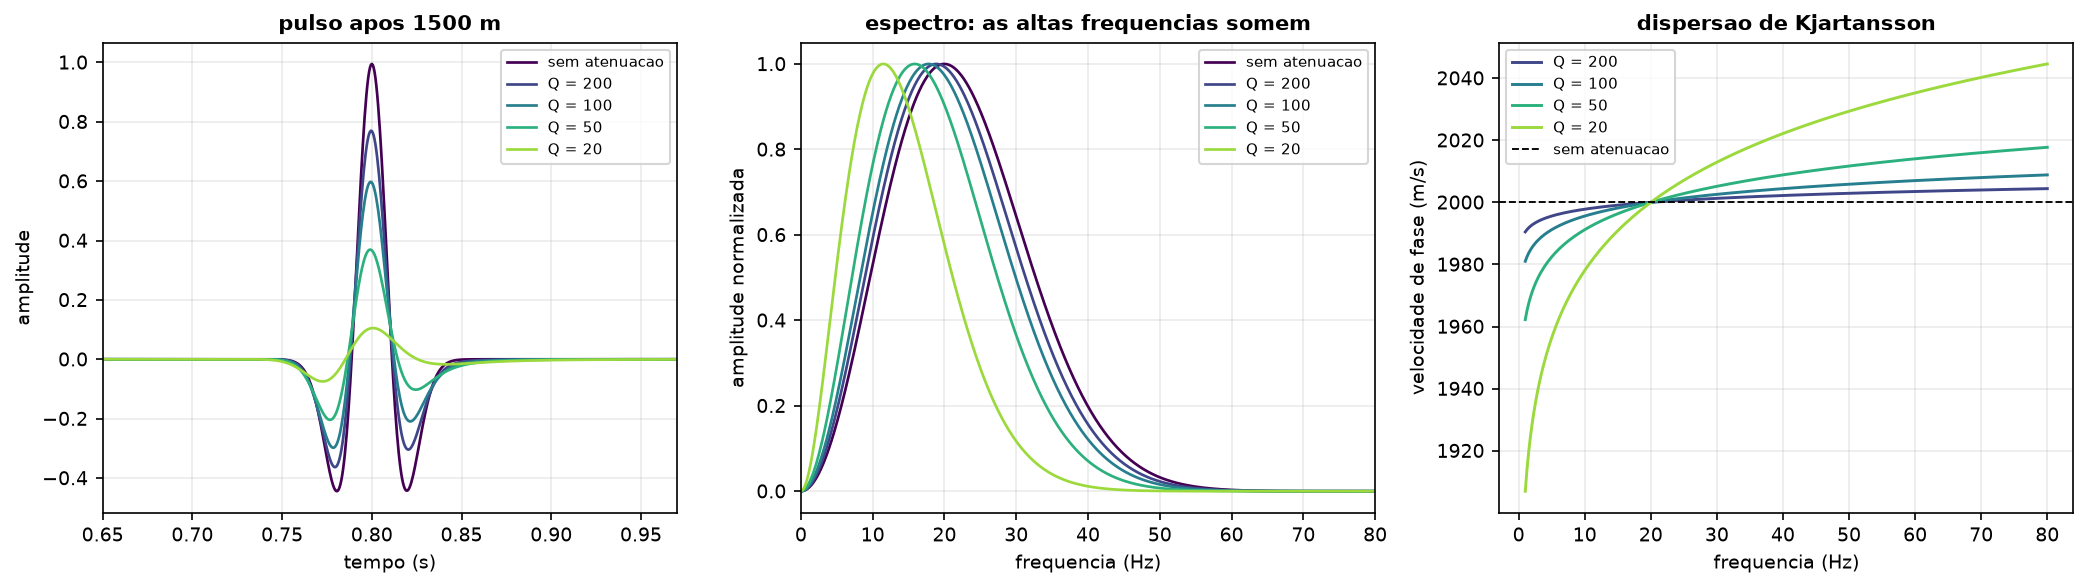
\includegraphics[width=0.96\textwidth]{../saidas/aula14/01_atenuacao_kjartansson.png}
\caption{Modelo constant-$Q$: pulso, espectro e dispers\~ao da velocidade de
fase. Os tr\^es efeitos --- perda de amplitude, descida da frequ\^encia de
pico e mudan\c{c}a de velocidade --- s\~ao insepar\'aveis, por causalidade.}
\end{figure}

\section{O princ\'ipio que organiza o cap\'itulo}
\label{sec:principio3}

\begin{armadilha}[]
\textbf{O que a FWI n\~ao consegue explicar pela f\'isica, ela explica mexendo
no modelo.}

Formalmente: se o dado cont\'em uma componente $\Delta$ fora da imagem de $F$,
o m\'inimo de $\tfrac12\norm{F(m)-d}^{2}$ \'e alcan\c{c}ado projetando $d$
sobre a imagem de $F$ --- e a proje\c{c}\~ao de um erro \emph{coerente} n\~ao
\'e ru\'ido: \'e uma estrutura leg\'itima do espa\c{c}o de modelos.

Isso explica por que erro de f\'isica produz modelos plaus\'iveis em vez de
artefatos \'obvios: a estrutura fabricada \'e, por constru\c{c}\~ao, a mais
compat\'ivel com a f\'isica adotada.
\end{armadilha}

\begin{pratica}[Como decidir de qual f\'isica voc\^e precisa]
\begin{enumerate}[leftmargin=*, itemsep=1pt]
\item \textbf{Olhe o res\'iduo, n\~ao $J$.} Estrutura coerente no res\'iduo
final \'e a assinatura de f\'isica faltando. Res\'iduo de aspecto aleat\'orio
significa que se chegou ao limite do dado.
\item \textbf{Espectro contra afastamento.} Sint\'etico com alta frequ\^encia
que o dado j\'a perdeu $\Rightarrow$ atenua\c{c}\~ao n\~ao modelada.
\item \textbf{Amplitude contra afastamento.} Decaimento mais r\'apido no dado
$\Rightarrow$ dissipa\c{c}\~ao ou espalhamento 3D.
\item \textbf{Eventos ausentes.} Energia em tempos onde o ac\'ustico n\~ao
produz nada $\Rightarrow$ ondas S, convers\~oes ou m\'ultiplas.
\item \textbf{Teste de f\'isica cruzada.} Gere o dado com a f\'isica completa,
inverta com a simples, me\c{c}a o erro de modelo. \'E a medida direta do custo
da aproxima\c{c}\~ao --- e o \'unico experimento que a justifica ou a
condena.
\end{enumerate}

\textbf{E o custo do caminho inverso:} mais f\'isica significa mais
par\^ametros, mais \emph{crosstalk}, mais m\'inimos locais e mais dificuldade
em atribuir um resultado a uma causa. A pergunta certa n\~ao \'e ``qual \'e a
f\'isica mais completa?'', e sim \textbf{``qual \'e a mais simples que explica
o meu dado?''}
\end{pratica}

\begin{resumo}
\begin{itemize}[leftmargin=*, itemsep=1pt]
\item \emph{Crosstalk} \'e a magnitude dos blocos $F_1'^{*}F_2'$ da Hessiana ---
uma quantidade calcul\'avel, n\~ao uma met\'afora.
\item Padr\~oes de radia\c{c}\~ao complementares (como $I_p$ e $c$) reduzem
\emph{crosstalk}; a reparametriza\c{c}\~ao \'e a ferramenta mais barata contra
ele, e n\~ao remove a ambiguidade --- realoca.
\item Se a aquisi\c{c}\~ao n\~ao cobre os \^angulos que separam dois
par\^ametros, nenhum m\'etodo os separa. \'E limita\c{c}\~ao de dado.
\item O adjunto viscoac\'ustico \'e est\'avel; inst\'avel \'e reconstruir o
campo \emph{direto} ao contr\'ario. S\~ao afirma\c{c}\~oes diferentes, e
confundi-las \'e comum.
\item Causalidade amarra dissipa\c{c}\~ao a dispers\~ao: n\~ao existe
corre\c{c}\~ao de amplitude que dispense corrigir a fase.
\end{itemize}
\end{resumo}

\begin{exercicio}[Problemas]
\begin{enumerate}[leftmargin=*, itemsep=2pt]
\item Deduza \eqref{eq:radiacao_Ic} a partir de \eqref{eq:radiacao} e das
rela\c{c}\~oes $\kappa = 1/(I_p c)$, $\rho = I_p/c$.
\item Usando \eqref{eq:radiacao_Ic}, determine o \^angulo de espalhamento em
que a sensibilidade a $c$ e a $I_p$ t\^em a mesma magnitude. O que isso diz
sobre a faixa de afastamentos que melhor separa os dois?
\item Um meio tem $Q = 60$, e o alvo est\'a a 4\,km de percurso, com
$c_0 = 2200$\,m/s e $f_{\text{ref}} = 15$\,Hz. Estime o erro de tempo de
tr\^ansito em 40\,Hz e compare com $T/2$.
\item Explique por que fixar $\epsilon$ e $\delta$ em invers\~ao VTI \'e uma
decis\~ao sobre a Hessiana, e n\~ao sobre a f\'isica.
\end{enumerate}
\textbf{Respostas.} (1) Substitua
$\delta\kappa/\kappa = -\delta I_p/I_p - \delta c/c$ e
$\delta\rho/\rho = \delta I_p/I_p - \delta c/c$ em \eqref{eq:radiacao} e
agrupe. (2) $\abs{\cos\theta-1} = \abs{1+\cos\theta}
\Rightarrow \cos\theta = 0 \Rightarrow \theta = 90^\circ$: \^angulos
intermedi\'arios --- nem incid\^encia normal (s\'o $I_p$) nem transmiss\~ao
pura (s\'o $c$). \'E o regime de afastamento m\'edio a longo. (3)
$\gamma = \arctan(1/60)/\pi \approx 5{,}3\times10^{-3}$;
$\delta t \approx (L/c_0)[1-(f/f_{\text{ref}})^{-\gamma}]
= (4000/2200)[1 - (40/15)^{-0{,}0053}] \approx 9{,}4$\,ms, contra
$T/2 = 12{,}5$\,ms em 40\,Hz: dentro do limite, mas com pouca margem --- e o
erro de \emph{amplitude} \'e adicional. (4) Porque a f\'isica VTI \'e
perfeitamente bem definida com os tr\^es par\^ametros; o que impede
invert\^e-los juntos \'e o mau condicionamento dos blocos cruzados para a
cobertura angular dispon\'ivel. Fixar \'e uma escolha de
regulariza\c{c}\~ao (um prior infinitamente forte), e deve ser declarada como
tal.
\end{exercicio}

% =====================================================================
\chapter{Diagn\'ostico e o que ainda n\~ao se sabe}
\label{cap:diagnostico}

\begin{ideia}
Um resultado de FWI n\~ao se valida mostrando que ele \'e bonito. Valida-se
tentando derrub\'a-lo --- e registrando o que sobreviveu. Este cap\'itulo
organiza os testes dispon\'iveis e delimita, com honestidade, o que nenhum
deles decide.
\end{ideia}

\section{A hierarquia de diagn\'osticos}

\begin{center}
\begin{tabular}{@{}p{4.6cm}p{6.0cm}p{4.2cm}@{}}
\toprule
\textbf{Diagn\'ostico} & \textbf{Responde} & \textbf{Custo} \\
\midrule
Teste do produto escalar & o adjunto est\'a certo?
  & desprez\'ivel \\
Teste de Taylor & o gradiente \'e a derivada do $J$ avaliado?
  & $\sim$10 modelagens \\
Res\'iduo final (imagem, n\~ao norma) & falta f\'isica?
  & zero (j\'a existe) \\
Espectro/amplitude \emph{versus} afastamento & atenua\c{c}\~ao, 3D, elasticidade?
  & zero \\
PSF em pontos-chave & qual \'e a resolu\c{c}\~ao \emph{aqui}?
  & 2 propaga\c{c}\~oes/tiro por ponto \\
Espectro de $H$ (Lanczos) & quais dire\c{c}\~oes o dado n\~ao restringe?
  & $k\times$ produtos $H\mathbf{v}$ \\
Passeio pelo espa\c{c}o nulo & existem modelos alternativos igualmente bons?
  & 1 modelagem por perturba\c{c}\~ao \\
Reinicia\c{c}\~ao de banda mais baixa & houve \emph{cycle skipping}?
  & uma invers\~ao inteira \\
\emph{Ensemble} (inicial, banda, $\lambda$, tiros) & o resultado \'e do dado ou
  das escolhas? & v\'arias invers\~oes \\
\bottomrule
\end{tabular}
\end{center}

\begin{teoria}[A assimetria que define a pr\'atica]
Os dois primeiros testes s\~ao \textbf{conclusivos}: h\'a uma resposta certa,
e o c\'odigo passa ou n\~ao. Todos os demais s\~ao \textbf{indicativos}:
reduzem a probabilidade de estar errado, sem elimin\'a-la.

Da\'i a regra pr\'atica: \emph{os testes conclusivos s\~ao obrigat\'orios e
baratos; os indicativos s\~ao caros e nenhum \'e suficiente sozinho}. Um
trabalho que reporta muitos diagn\'osticos indicativos e nenhum conclusivo n\~ao
estabeleceu nada sobre a corre\c{c}\~ao do c\'odigo.
\end{teoria}

\section{Sintomas e causas}

\begin{center}
\begin{tabular}{@{}p{3.6cm}p{11.2cm}@{}}
\toprule
\textbf{Sintoma} & \textbf{Investigar, nesta ordem} \\
\midrule
$J$ n\~ao cai & gradiente (teste de Taylor); dire\c{c}\~ao de descida
  ($\inner{\mathbf{g}}{\mathbf{d}}<0$?); sinal e par\^ametro do gradiente;
  escala do passo inicial \\
$J$ cai, modelo errado & \emph{cycle skipping} (reinicie mais baixo);
  $m_0$ fora do vale (Eq.~\ref{eq:tolerancia3}); f\'isica faltando (res\'iduo
  coerente?); ondaleta absorvendo erro; bordas \\
s\'o o raso atualiza & m\'ascara de aquisi\c{c}\~ao; pr\'e-condicionamento;
  abertura insuficiente (e isso nenhum algoritmo resolve) \\
\texttt{NaN} & CFL; modelo fora da caixa \emph{dentro} da busca linear \\
cauda oscilat\'oria & $G$ insuficiente; se $G$ j\'a \'e alto, \'e $\Delta t$;
  confirme em meio homog\^eneo \\
raz\~ao de Taylor est\'avel $\ne 1$ & adjunto de um pr\'e-processamento omitido
  ($E^{T}$); adjunto de CPML; discrep\^ancia cont\'inuo/discreto
  (teste refinando) \\
gradiente de um par\^ametro id\^entico a zero & regra da cadeia, n\~ao
  adjunto --- verifique $\partial\mathcal{A}/\partial p_k$ \\
\bottomrule
\end{tabular}
\end{center}

\section{O que se sabe que n\~ao se sabe}

\begin{teoria}[Problemas abertos, enunciados sem otimismo]
\textbf{1. N\~ao h\'a garantia de converg\^encia global.} Nenhum funcional
alternativo conhecido \'e convexo em $\mvec$ --- apenas mais bem comportado em
rela\c{c}\~ao a \emph{deslocamento}, que \'e uma propriedade bem mais fraca.
Transporte \'otimo, AWI e envolt\'oria ampliam bacias de atra\c{c}\~ao;
nenhum elimina m\'inimos locais.

\textbf{2. A lacuna espectral \'e propriedade do dado.} Por
\eqref{eq:km}, nenhuma escolha de algoritmo cria informa\c{c}\~ao abaixo de
$(4\pi f_{\min}/c)\sin(\theta_{\min}/2)$. Isso \'e um limite de
\emph{aquisi\c{c}\~ao}, e s\'o se resolve em campo --- fontes de baixa
frequ\^encia ou aberturas maiores.

\textbf{3. Erro de modelagem n\~ao \'e ru\'ido.} A formula\c{c}\~ao
estat\'istica padr\~ao assume ru\'ido aleat\'orio; f\'isica faltante \'e
\emph{determin\'istica e coerente}. Tratar as duas com a mesma covari\^ancia
$C_d$ \'e teoricamente indefens\'avel e universalmente praticado. Existe
literatura sobre covari\^ancia de erro de modelo; ela n\~ao \'e rotina.

\textbf{4. UQ em escala real est\'a fora de alcance.} A aproxima\c{c}\~ao de
Laplace \'e local e condicional \`a bacia; MCMC em dimens\~ao realista \'e
invi\'avel. O que se reporta hoje como ``incerteza'' em FWI 3D \'e, quase
sempre, variabilidade sobre escolhas metodol\'ogicas --- o que \'e \'util e
\emph{n\~ao} \'e uma distribui\c{c}\~ao a posteriori.

\textbf{5. Multipar\^ametro segue limitado por \^angulo, n\~ao por
algoritmo.} Se dois par\^ametros produzem dado indistingu\'ivel na faixa
angular iluminada, nenhuma regulariza\c{c}\~ao, parametriza\c{c}\~ao ou
m\'etodo de segunda ordem os separa. Reparametrizar realoca a ambiguidade;
n\~ao a remove.

\textbf{6. Escolher a f\'isica continua sendo julgamento.} Existem
diagn\'osticos (§\ref{sec:principio3}) mas n\~ao existe crit\'erio autom\'atico que decida se
vale pagar por viscoelasticidade num dado espec\'ifico.
\end{teoria}

\begin{pratica}[As cinco perguntas, na vers\~ao deste volume]
\begin{enumerate}[leftmargin=*, itemsep=2pt]
\item O teste do produto escalar e o de Taylor passaram? Com quais n\'umeros?
\item Qual era o erro do modelo inicial, e como ele foi obtido?
\item O res\'iduo final \'e incoerente? (Se tem estrutura, falta f\'isica ---
n\~ao houve converg\^encia, houve parada.)
\item Qual \'e a PSF nos pontos de interesse? A fei\c{c}\~ao que estou
interpretando \'e maior que ela?
\item O resultado sobrevive a mudan\c{c}as de banda inicial, modelo inicial e
$\lambda$? Se n\~ao, quem determinou a resposta foi a escolha, n\~ao o dado.
\end{enumerate}
\end{pratica}

\begin{resumo}
\begin{itemize}[leftmargin=*, itemsep=1pt]
\item Dois diagn\'osticos s\~ao \emph{conclusivos} (produto escalar, Taylor) e
baratos; todos os demais s\~ao indicativos e caros.
\item A PSF \'e a medida local de resolu\c{c}\~ao mais barata que n\~ao exige
conhecer a verdade --- e portanto serve em dado real.
\item Barras de erro de Laplace s\~ao condicionais \`a bacia e \`a f\'isica;
sem esse condicional, s\~ao enganosas.
\item O que permanece aberto n\~ao \'e detalhe de implementa\c{c}\~ao:
converg\^encia global, lacuna espectral, erro de modelagem como ru\'ido, UQ em
escala real, e ambiguidade multipar\^ametro limitada por \^angulo.
\end{itemize}
\end{resumo}

% =====================================================================
\appendix

\chapter{Nota\c{c}\~ao}

\begin{center}
\begin{longtable}{@{}ll@{}}
\toprule
\textbf{S\'imbolo} & \textbf{Significado} \\
\midrule
\endhead
$\mathcal{M},\mathcal{D}$ & espa\c{c}os de Hilbert de modelos e de dados \\
$\mvec$, $m = 1/c^{2}$ & modelo; vagarosidade ao quadrado \\
$F$, $F'$, $F'^{*}$ & operador direto; derivada de Fr\'echet (Born); seu adjunto \\
$\mathcal{A}(m)$ & operador de onda; $\mathcal{A}_\omega = -\omega^{2}m-\nabla^{2}$ \\
$R$ & operador de restri\c{c}\~ao aos receptores \\
$G$ & fun\c{c}\~ao de Green \\
$\lambda(\mathbf{x},t)$ & campo adjunto \\
$\delta p,\ \delta\lambda$ & campos tangente linear e adjunto de 2\textsuperscript{a} ordem \\
$H$, $H_{\text{GN}} = F'^{*}F'$ & Hessiana e sua aproxima\c{c}\~ao de Gauss--Newton \\
$C_d$, $C_m$, $C_{\text{post}}$ & covari\^ancias do ru\'ido, do prior e a posteriori \\
$\mathbf{k}_i,\mathbf{k}_s,\mathbf{k}_m$ & n\'umeros de onda incidente,
  espalhado e do modelo \\
$\theta$ & \^angulo de espalhamento ($\pi$ = retroespalhamento) \\
$\vartheta = \pi-\theta$ & \^angulo de abertura fonte--receptor \\
$S(\theta)$ & s\'imbolo do est\^encil espacial \\
$C$, $C_{\lim}$, $G$ & Courant, seu limite, e pontos por comprimento de onda \\
$s(x)$ & fator de estiramento complexo da PML \\
$\gamma$, $Q$ & expoente de Kjartansson e fator de qualidade \\
$I_p = \rho c$, $\kappa = 1/K$ & imped\^ancia e compressibilidade \\
$E$ & operador linear de pr\'e-processamento do modelo \\
$\mathcal{H}$ & transformada de Hilbert \\
$W_2$ & dist\^ancia de Wasserstein quadr\'atica \\
\bottomrule
\end{longtable}
\end{center}

\begin{atencao}[Colis\~oes herdadas da literatura]
$\lambda$ \'e par\^ametro de Lam\'e, campo adjunto, peso de regulariza\c{c}\~ao
e comprimento de onda; $\mu$ \'e m\'odulo de cisalhamento e par\^ametro de
penalidade da WRI; $G$ \'e fun\c{c}\~ao de Green e pontos por comprimento de
onda; $J$ \'e o funcional e $J' = F'$ a jacobiana do \emph{res\'iduo}. O
contexto resolve, mas a colis\~ao \'e da \'area.
\end{atencao}

\chapter{Identidades usadas}

\textbf{Integra\c{c}\~ao por partes no tempo.}
\[
\int_0^T \lambda\,\partial_{tt}\varphi \dd t
 = \bigl[\lambda\,\partial_t\varphi - \partial_t\lambda\,\varphi\bigr]_0^T
 + \int_0^T \partial_{tt}\lambda\;\varphi \dd t .
\]

\textbf{Segunda identidade de Green.}
\[
\int_\Omega \bigl(\lambda\nabla^{2}\varphi - \varphi\nabla^{2}\lambda\bigr)
 \dd\mathbf{x}
 = \oint_{\partial\Omega}\bigl(\lambda\,\partial_n\varphi
 - \varphi\,\partial_n\lambda\bigr)\dd S .
\]

\textbf{Adjuntos elementares.}
$\partial_t^{*} = -\partial_t$; $\partial_{tt}^{*} = \partial_{tt}$;
$(\nabla^{2})^{*} = \nabla^{2}$ com contorno homog\^eneo;
$\mathcal{H}^{*} = -\mathcal{H}$; $D^{*} = D^{T}$ para qualquer matriz.
\textbf{Toda matriz diagonal \'e auto-adjunta} --- da\'i o Cerjan.

\textbf{Transformada de Fourier} (conven\c{c}\~ao usada).
$\hat w(f) = \int w(t)e^{-2\pi\mathrm{i}ft}\dd t$;
$\widehat{\partial_t w} = \mathrm{i}\omega\,\hat w$ com $\omega = 2\pi f$;
$\widehat{w(\cdot-t_0)} = \hat w\,e^{-2\pi\mathrm{i}ft_0}$.

\textbf{Espectro da Ricker.}
$\abs{W(f)} = (2/\sqrt{\pi})(f^{2}/f_0^{3})e^{-f^{2}/f_0^{2}}$; pico em $f_0$;
$-6$\,dB em $1{,}64f_0$; $-20$\,dB em $2{,}21f_0$ (ra\'izes de
$u\,e^{1-u} = \eta$ com $u = (f/f_0)^{2}$).

\textbf{Estabilidade e dispers\~ao (leap-frog $+$ est\^encil centrado).}
\[
C_{\lim} = \frac{2}{\sqrt{n_{\dim}\bigl(\abs{c_0}+2\sum_j\abs{c_j}\bigr)}},
\qquad
\frac{4}{\Delta t^{2}}\sin^{2}\frac{\omega\Delta t}{2}
 = \frac{c^{2}}{\Delta h^{2}}\sum_j S(k_j\Delta h).
\]

\textbf{Cobertura de n\'umero de onda.}
$\abs{\mathbf{k}_m} = (4\pi/\lambda)\sin(\theta/2)$.

\textbf{Radia\c{c}\~ao P--P ac\'ustica.}
$f(\theta)\propto \delta\kappa/\kappa + (\delta\rho/\rho)\cos\theta$;
em $(I_p,c)$,
$f(\theta)\propto (\delta I_p/I_p)(\cos\theta-1) - (\delta c/c)(1+\cos\theta)$.

\textbf{Desajuste sob deslocamento puro.}
$\Phi(\tau) = \norm{d}^{2} - R_{dd}(\tau)$.

\chapter{Refer\^encias}

\begin{enumerate}[leftmargin=*, itemsep=3pt]
\item ASNAASHARI, A. \emph{et al.} \emph{Regularized seismic full waveform
inversion with prior model information.} Geophysics, v.~78, n.~2,
p.~R25--R36, 2013.

\item BUNKS, C.; SALECK, F.~M.; ZALESKI, S.; CHAVENT, G. \emph{Multiscale
seismic waveform inversion.} Geophysics, v.~60, n.~5, p.~1457--1473, 1995.

\item CARCIONE, J.~M. \emph{Wave Fields in Real Media.} 4.~ed. Elsevier, 2022.

\item CERJAN, C. \emph{et al.} \emph{A nonreflecting boundary condition for
discrete acoustic and elastic wave equations.} Geophysics, v.~50, n.~4,
p.~705--708, 1985.

\item CHEN, P.; JORDAN, T.~H.; ZHAO, L. \emph{Full three-dimensional
tomography: a comparison between the scattering-integral and adjoint-wavefield
methods.} Geophysical Journal International, v.~170, n.~1, p.~175--181, 2007.

\item ESSER, E.; GUASCH, L.; VAN LEEUWEN, T.; ARAVKIN, A.~Y.; HERRMANN, F.~J.
\emph{Total variation regularization strategies in full-waveform inversion.}
SIAM Journal on Imaging Sciences, v.~11, n.~1, p.~376--406, 2018.

\item FICHTNER, A. \emph{Full Seismic Waveform Modelling and Inversion.}
Springer, 2011.

\item GEBRAAD, L.; BOEHM, C.; FICHTNER, A. \emph{Bayesian elastic
full-waveform inversion using Hamiltonian Monte Carlo.} Journal of Geophysical
Research: Solid Earth, v.~125, n.~3, e2019JB018428, 2020.

\item GRIEWANK, A.; WALTHER, A. \emph{Algorithm 799: revolve --- an
implementation of checkpointing for the reverse or adjoint mode of
computational differentiation.} ACM TOMS, v.~26, n.~1, p.~19--45, 2000.

\item GRIEWANK, A.; WALTHER, A. \emph{Evaluating Derivatives: Principles and
Techniques of Algorithmic Differentiation.} 2.~ed. SIAM, 2008. --- o
tratamento completo do resultado de \emph{checkpointing} \'otimo.

\item KJARTANSSON, E. \emph{Constant-Q wave propagation and attenuation.}
JGR, v.~84, p.~4737--4748, 1979.

\item KOMATITSCH, D.; MARTIN, R. \emph{An unsplit convolutional perfectly
matched layer improved at grazing incidence for the seismic wave equation.}
Geophysics, v.~72, n.~5, p.~SM155--SM167, 2007.

\item KREBS, J.~R. \emph{et al.} \emph{Fast full-wavefield seismic inversion
using encoded sources.} Geophysics, v.~74, n.~6, p.~WCC177--WCC188, 2009.

\item LUO, Y.; SCHUSTER, G.~T. \emph{Wave-equation traveltime inversion.}
Geophysics, v.~56, n.~5, p.~645--653, 1991.

\item MARQUERING, H.; DAHLEN, F.~A.; NOLET, G. \emph{Three-dimensional
sensitivity kernels for finite-frequency traveltimes: the banana-doughnut
paradox.} Geophysical Journal International, v.~137, n.~3, p.~805--815, 1999.

\item M\'ETIVIER, L.; BROSSIER, R.; VIRIEUX, J.; OPERTO, S.
\emph{Full waveform inversion and the truncated Newton method.} SIAM Journal
on Scientific Computing, v.~35, n.~2, p.~B401--B437, 2013.

\item M\'ETIVIER, L. \emph{et al.} \emph{Measuring the misfit between
seismograms using an optimal transport distance.} Geophysical Journal
International, v.~205, n.~1, p.~345--377, 2016.

\item MORGAN, J. \emph{et al.} \emph{Next-generation seismic experiments:
wide-angle, multi-azimuth, three-dimensional, full-waveform inversion.}
Geophysical Journal International, v.~195, n.~3, p.~1657--1678, 2013.

\item NOCEDAL, J.; WRIGHT, S.~J. \emph{Numerical Optimization.} 2.~ed.
Springer, 2006.

\item OPERTO, S. \emph{et al.} \emph{A guided tour of multiparameter
full-waveform inversion with multicomponent data.} The Leading Edge, v.~32,
n.~9, p.~1040--1054, 2013.

\item PLED, F.; DESCELIERS, C. \emph{Review and recent developments on the
perfectly matched layer (PML) method for the numerical modeling and simulation
of elastic wave propagation in unbounded domains.} Archives of Computational
Methods in Engineering, v.~29, n.~1, p.~471--518, 2022.

\item PLESSIX, R.-E. \emph{A review of the adjoint-state method for computing
the gradient of a functional with geophysical applications.} GJI, v.~167,
n.~2, p.~495--503, 2006.

\item PRATT, R.~G. \emph{Seismic waveform inversion in the frequency domain,
Part 1.} Geophysics, v.~64, n.~3, p.~888--901, 1999.

\item SCH\"AFER, M.; GROOS, L.; FORBRIGER, T.; BOHLEN, T. \emph{Line-source
simulation for shallow-seismic data. Part 2: full-waveform inversion --- a
synthetic 2-D case study.} Geophysical Journal International, v.~198, n.~3,
p.~1405--1418, 2014.

\item SHIN, C.; JANG, S.; MIN, D.-J. \emph{Improved amplitude preservation for
prestack depth migration by inverse scattering theory.} Geophysical
Prospecting, v.~49, n.~5, p.~592--606, 2001.

\item SIRGUE, L.; PRATT, R.~G. \emph{Efficient waveform inversion and imaging:
a strategy for selecting temporal frequencies.} Geophysics, v.~69, n.~1,
p.~231--248, 2004.

\item SYMES, W.~W. \emph{Migration velocity analysis and waveform inversion.}
Geophysical Prospecting, v.~56, n.~6, p.~765--790, 2008.

\item TARANTOLA, A. \emph{Inversion of seismic reflection data in the acoustic
approximation.} Geophysics, v.~49, n.~8, p.~1259--1266, 1984.

\item TARANTOLA, A. \emph{A strategy for nonlinear elastic inversion of
seismic reflection data.} Geophysics, v.~51, n.~10, p.~1893--1903, 1986.

\item TARANTOLA, A. \emph{Inverse Problem Theory and Methods for Model
Parameter Estimation.} SIAM, 2005.

\item TROMP, J.; TAPE, C.; LIU, Q. \emph{Seismic tomography, adjoint methods,
time reversal and banana-doughnut kernels.} GJI, v.~160, n.~1, p.~195--216,
2005.

\item VAN LEEUWEN, T.; HERRMANN, F.~J. \emph{Mitigating local minima in
full-waveform inversion by expanding the search space.} GJI, v.~195, n.~1,
p.~661--667, 2013.

\item VIRIEUX, J.; OPERTO, S. \emph{An overview of full-waveform inversion in
exploration geophysics.} Geophysics, v.~74, n.~6, p.~WCC1--WCC26, 2009.

\item VIRIEUX, J.; ASNAASHARI, A.; BROSSIER, R.; M\'ETIVIER, L.; RIBODETTI,
A.; ZHOU, W. \emph{An introduction to full waveform inversion.} In:
\emph{Encyclopedia of Exploration Geophysics}. Tulsa: SEG, 2014.
p.~R1-1--R1-40. DOI 10.1190/1.9781560803027.entry6.

\item WARNER, M.; GUASCH, L. \emph{Adaptive waveform inversion: theory.}
Geophysics, v.~81, n.~6, p.~R429--R445, 2016.

\item WU, R.-S.; TOKS\"OZ, M.~N. \emph{Diffraction tomography and multisource
holography applied to seismic imaging.} Geophysics, v.~52, n.~1, p.~11--25,
1987.
\end{enumerate}

\vfill
\begin{center}
{\color{cianofwi}\rule{0.55\textwidth}{1pt}}\\[0.35cm]
{\small Volume 3 de 3 $\cdot$ os tr\^es volumes compartilham a mesma estrutura
de cap\'itulos.\\
Figuras e n\'umeros gerados pelo c\'odigo em \arq{aulas/} e \arq{fwikit/}.}
\end{center}

\end{document}
